\documentclass[main]{subfiles}

\begin{document}
% Chapter Template
\setcounter{chapter}{3}

% Results
%  Creatures with uncoupled sinusoidal oscillators
%  Simple limiter control in the simulator
%   Indirect limiter control through the morphology
%   Direct limiter control through the sensor feedback
%    Limiting the Model Leg in the Minemonics simulator
%    Evolved examples 
\chapter{Results} % Main chapter title

\label{Chapter\thechapter} % Change X to a consecutive number; for referencing this chapter elsewhere, use \ref{ChapterX}

\lhead{Chapter \thechapter. \emph{Results}} % Change X to a consecutive number; this is for the header on each page - perhaps a shortened title

\section{Evolved Creatures with Uncoupled Sinusoidal Controller}
\label{sec:evolved-sin-creatures}

In the first experimental setting, the sinusoidal controller as described in \ref{sec:sinusoidal-controllers} was used to evolve creatures. %
%
A population of 100 creatures was set up with an average velocity fitness function and a minimal height fitness function. %
%
The latter was chosen because the simulator had issues in the physical model setup that led to creatures with the ability to fly due to imaginary forces (as described in \ref{subsec:populations}). %
%
The minimal height fitness function punished those creatures that reached a high average height, which is the case for creatures that are flying. %
%
The simulation was run for approximately a day and took 181 generations for locomotion behavior to occur. %
%
Every creature was evaluated for 20 seconds. %
%
181 generations of 100 creatures evaluated for 20 seconds take \(\approx\unit[4.2]{days}\), however, since the simulator can evaluate faster than real-time if the simulation's load permits it, it could simulate the creatures \(\approx\unit[4.2]{}\) faster than real-time. %
%
The successful solutions evolved can be seen below in figures \ref{figure:successfulcreatures-jumper1}, \ref{figure:successfulcreatures-jumper2}, \ref{figure:successfulcreatures-walker1} and \ref{figure:successfulcreatures-walker2}.

\begin{figure}[tb]
\centering
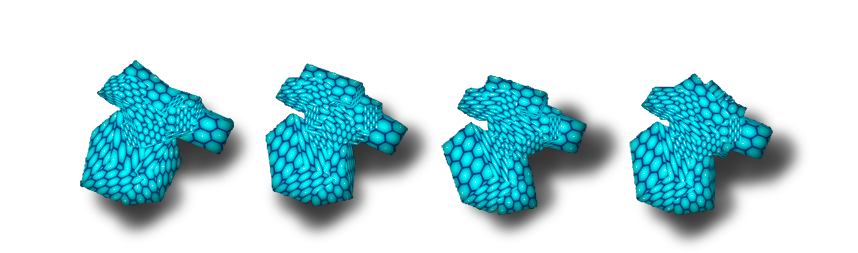
\includegraphics[width=0.9\textwidth]{results/evolved-creatures/sine/jumper1/jumper1-animation.png}
%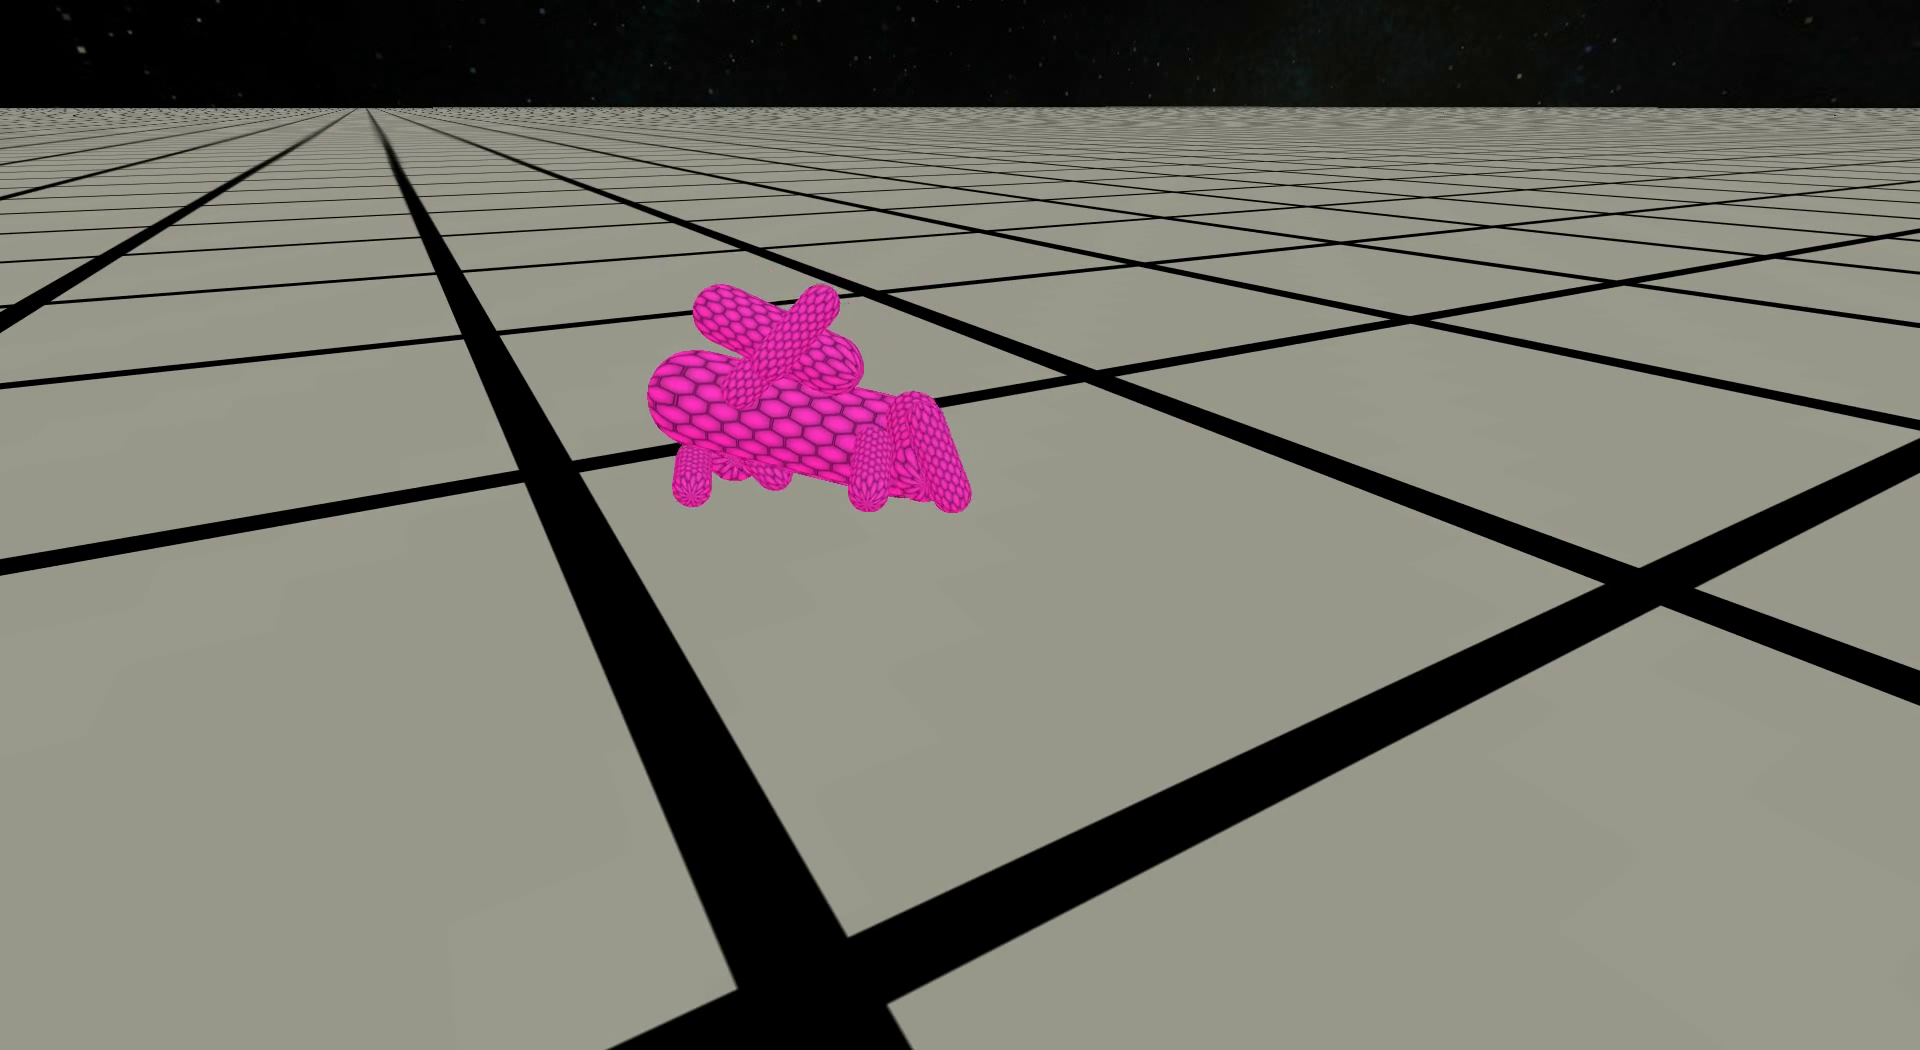
\includegraphics[width=0.45\textwidth]{results/evolved-creatures/sine/jumper1/165.png}
%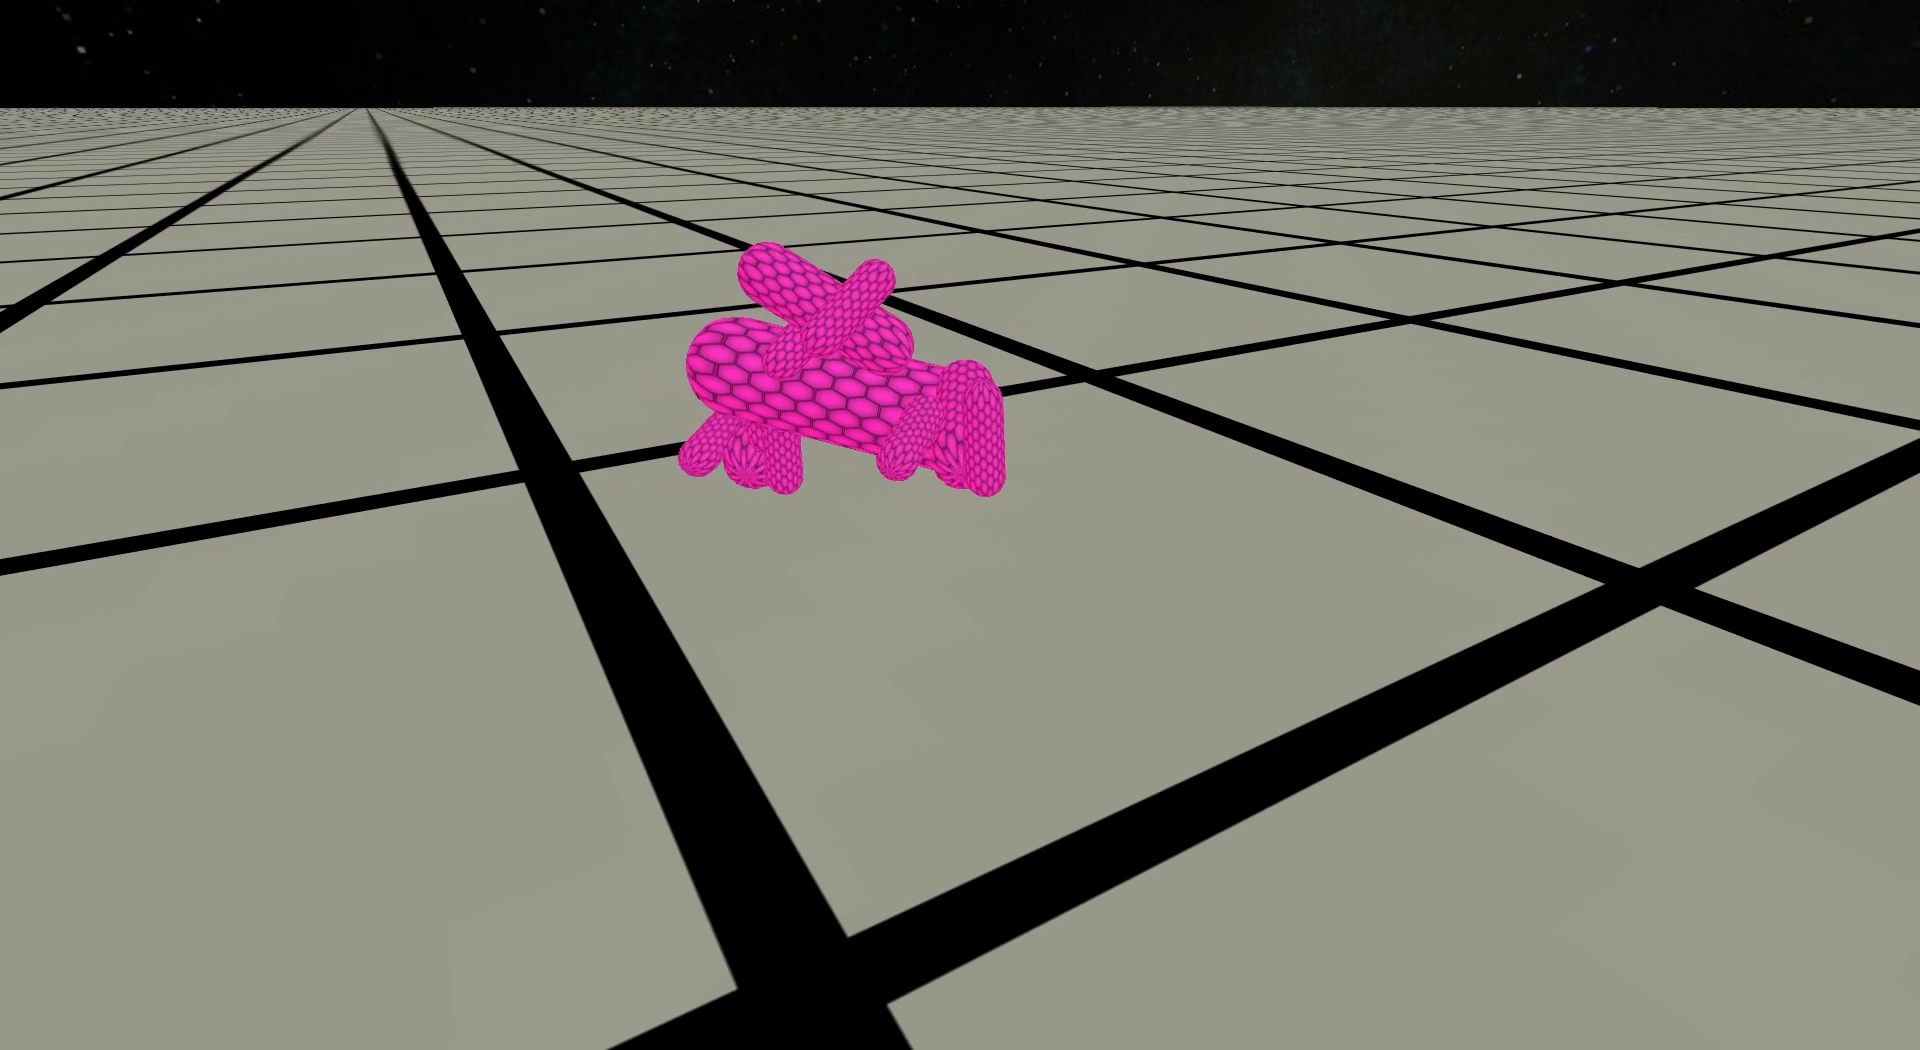
\includegraphics[width=0.45\textwidth]{results/evolved-creatures/sine/jumper1/179.png}
%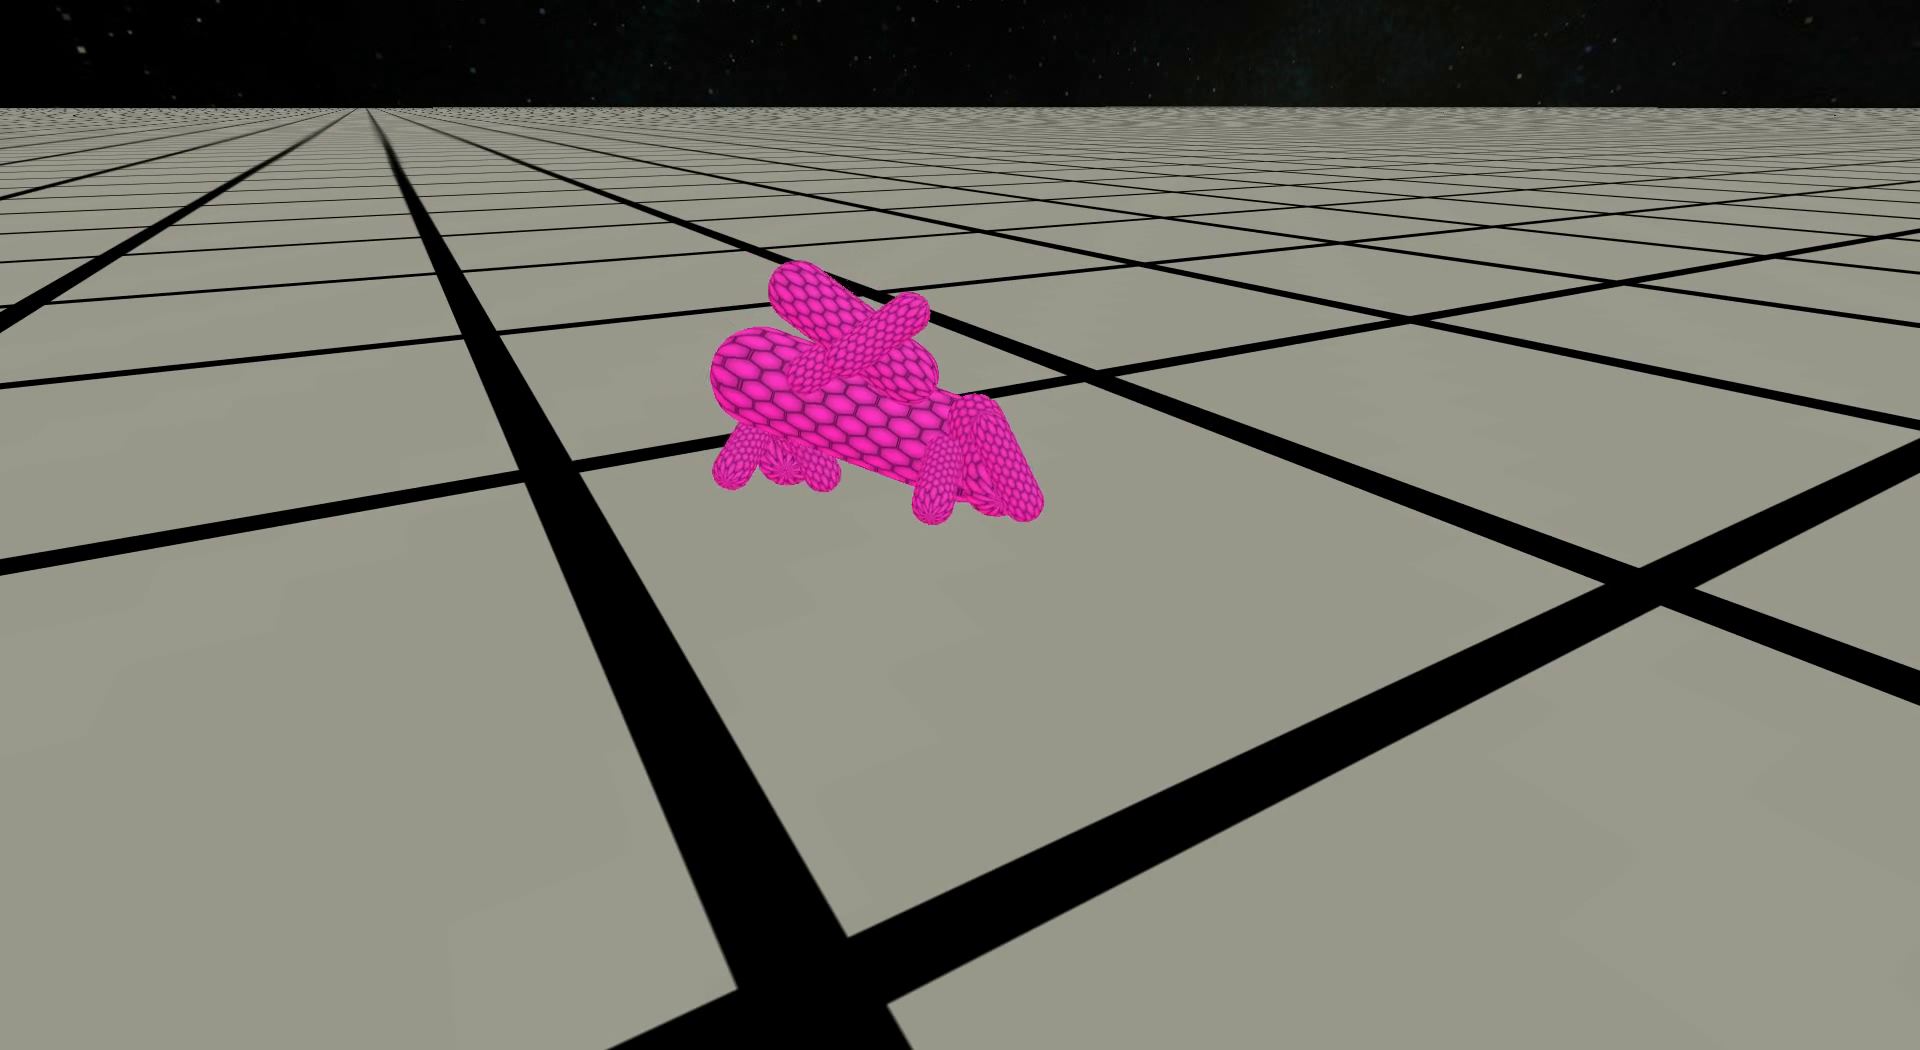
\includegraphics[width=0.45\textwidth]{results/evolved-creatures/sine/jumper1/188.png}
%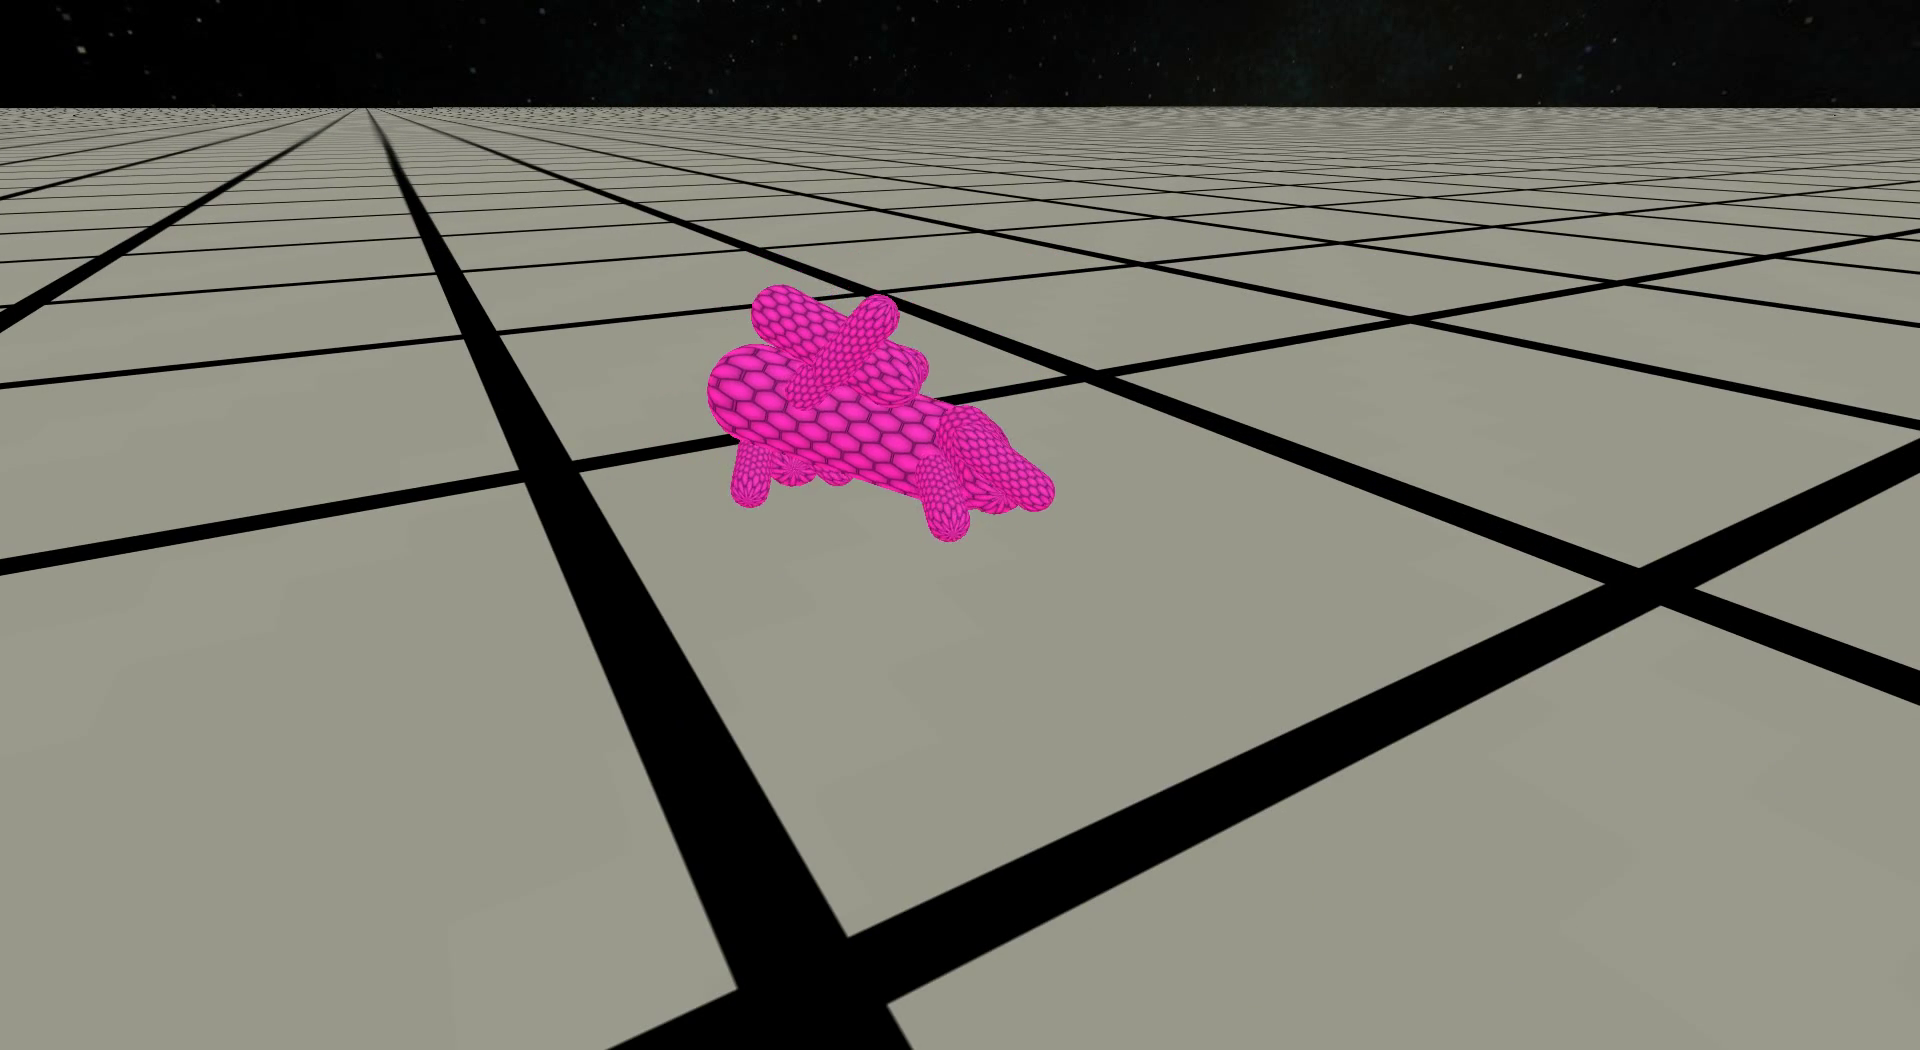
\includegraphics[width=0.45\textwidth]{results/evolved-creatures/sine/jumper1/196.png}
\caption[Figure of a jumper using sinusoidal controllers.]{Figure of a jumper using sinusoidal controllers. Its four legs under the main body let it leap forward. A video of the jumping creature can be found on YouTube: \url{https://youtu.be/jMHQnsCy8_k}.}
\label{figure:successfulcreatures-jumper1}
\end{figure}

\begin{figure}[tb]
\centering
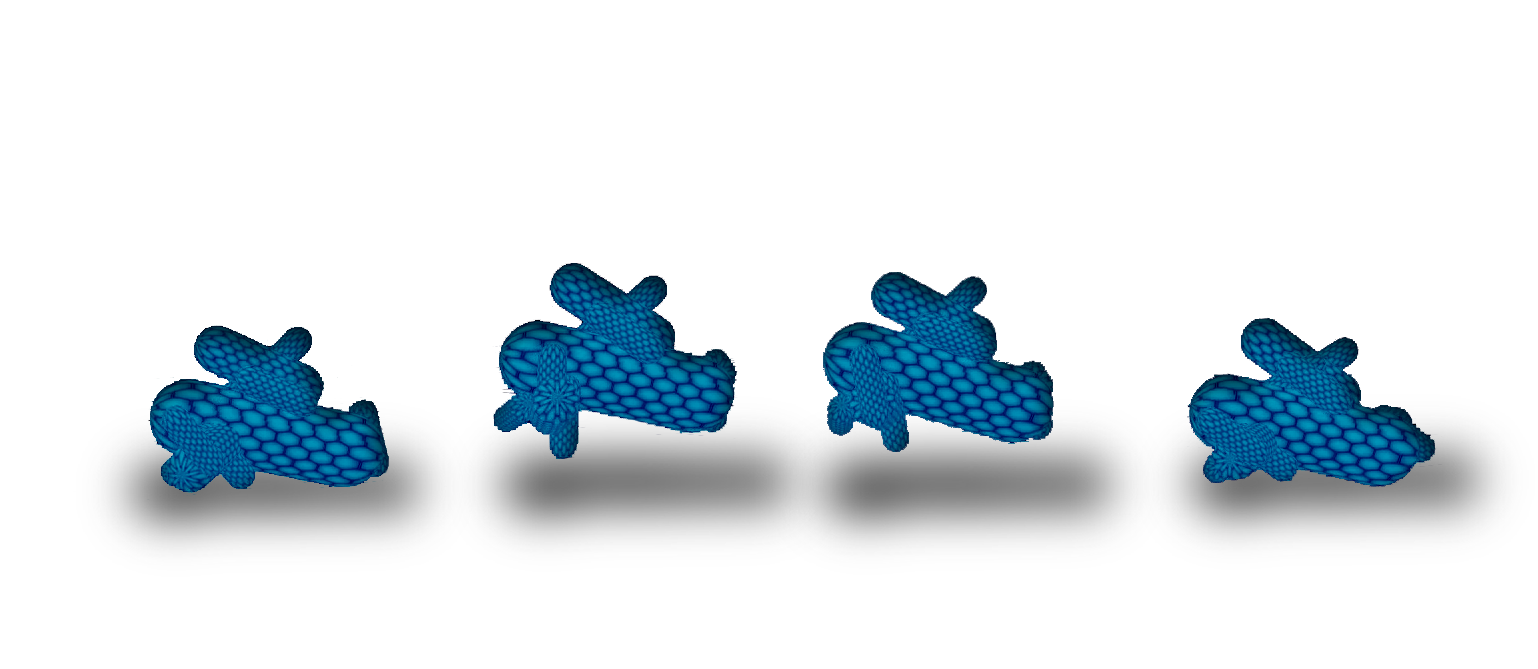
\includegraphics[width=0.95\textwidth]{results/evolved-creatures/sine/jumper2/jumper2-animation.png}
%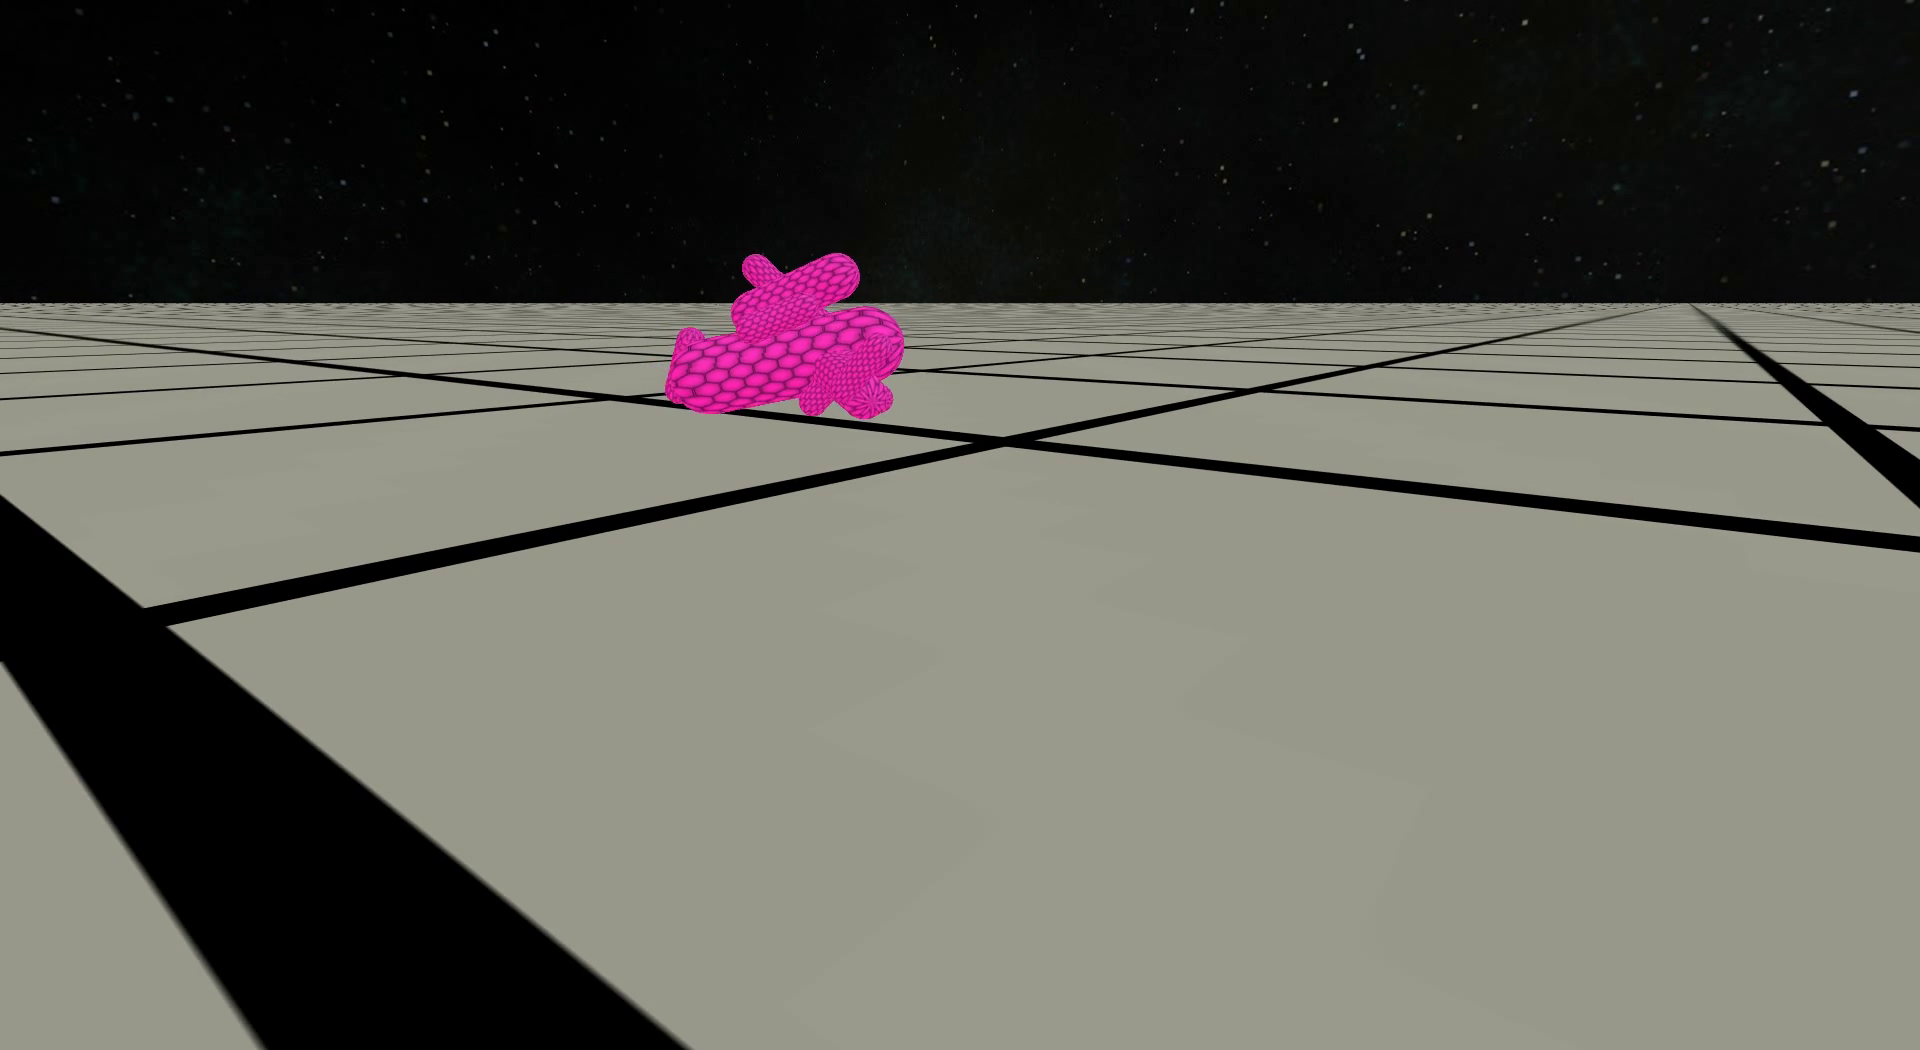
\includegraphics[width=0.45\textwidth]{results/evolved-creatures/sine/jumper2/336.png}
%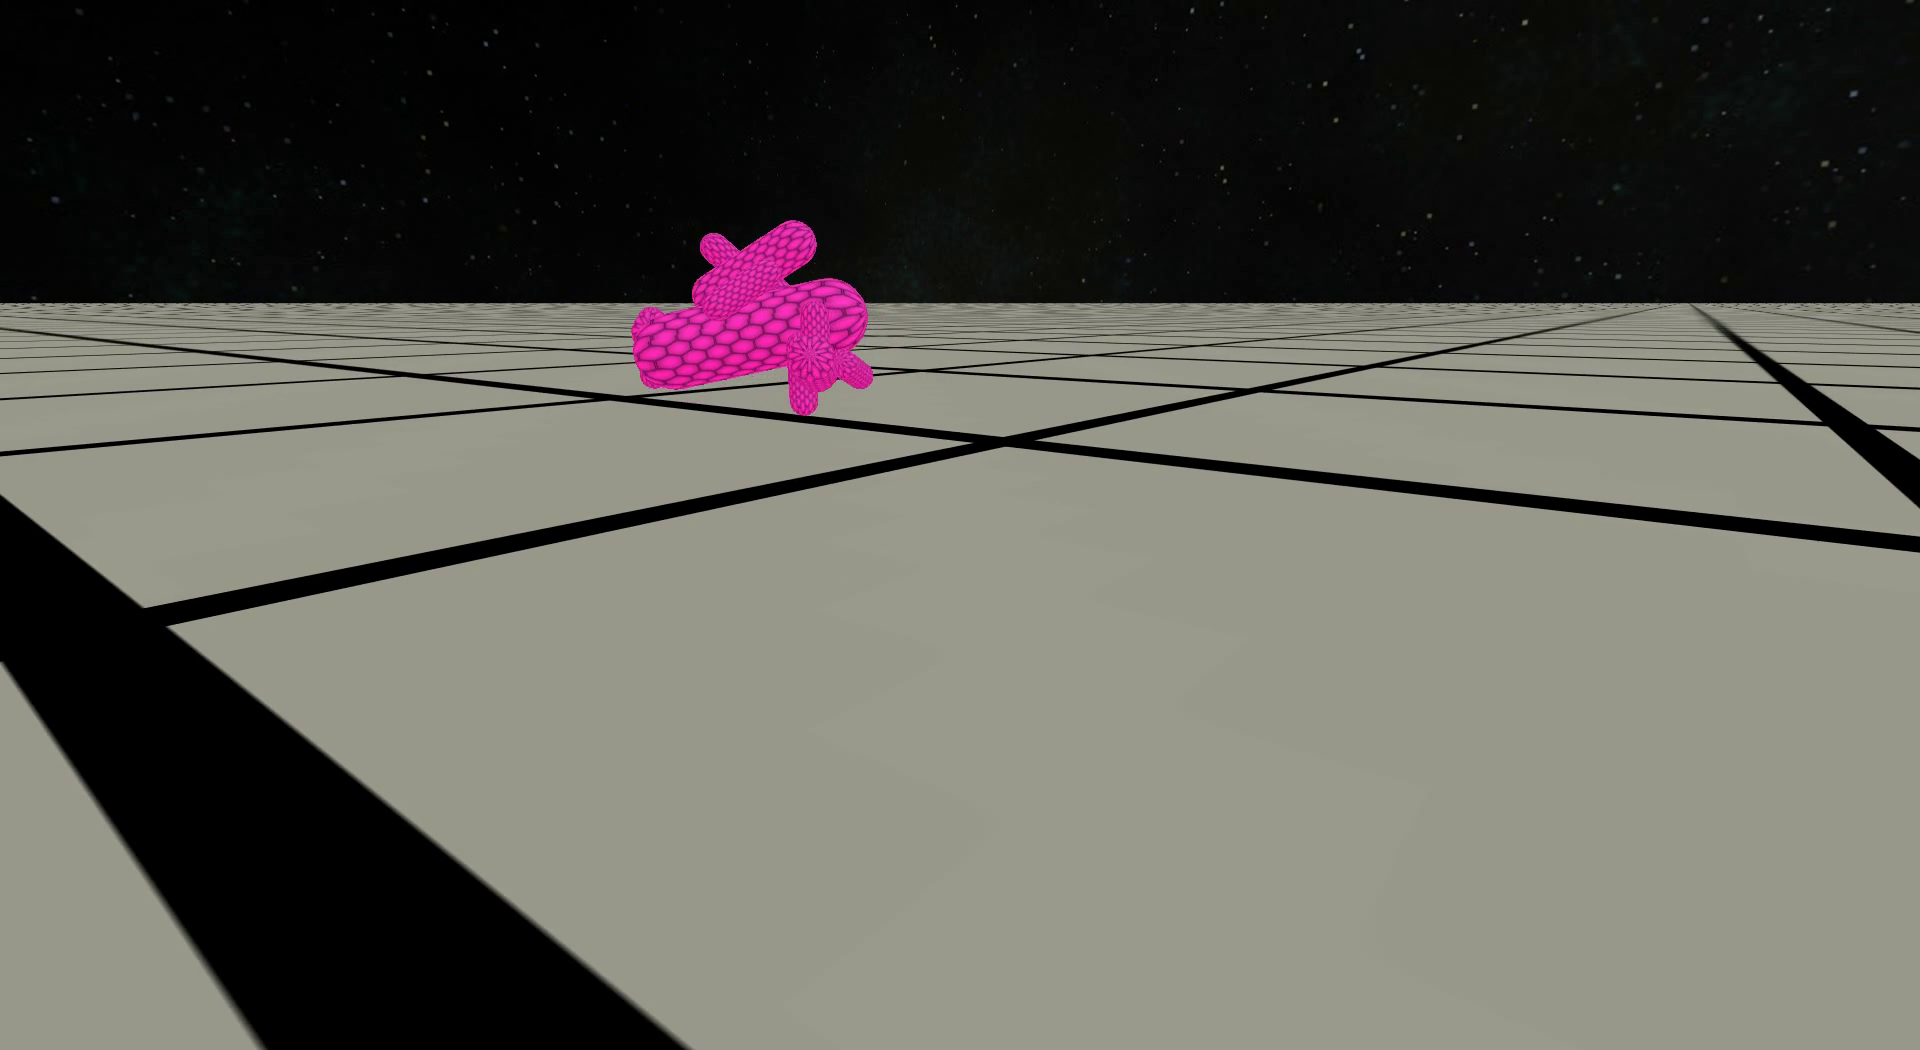
\includegraphics[width=0.45\textwidth]{results/evolved-creatures/sine/jumper2/359.png}
%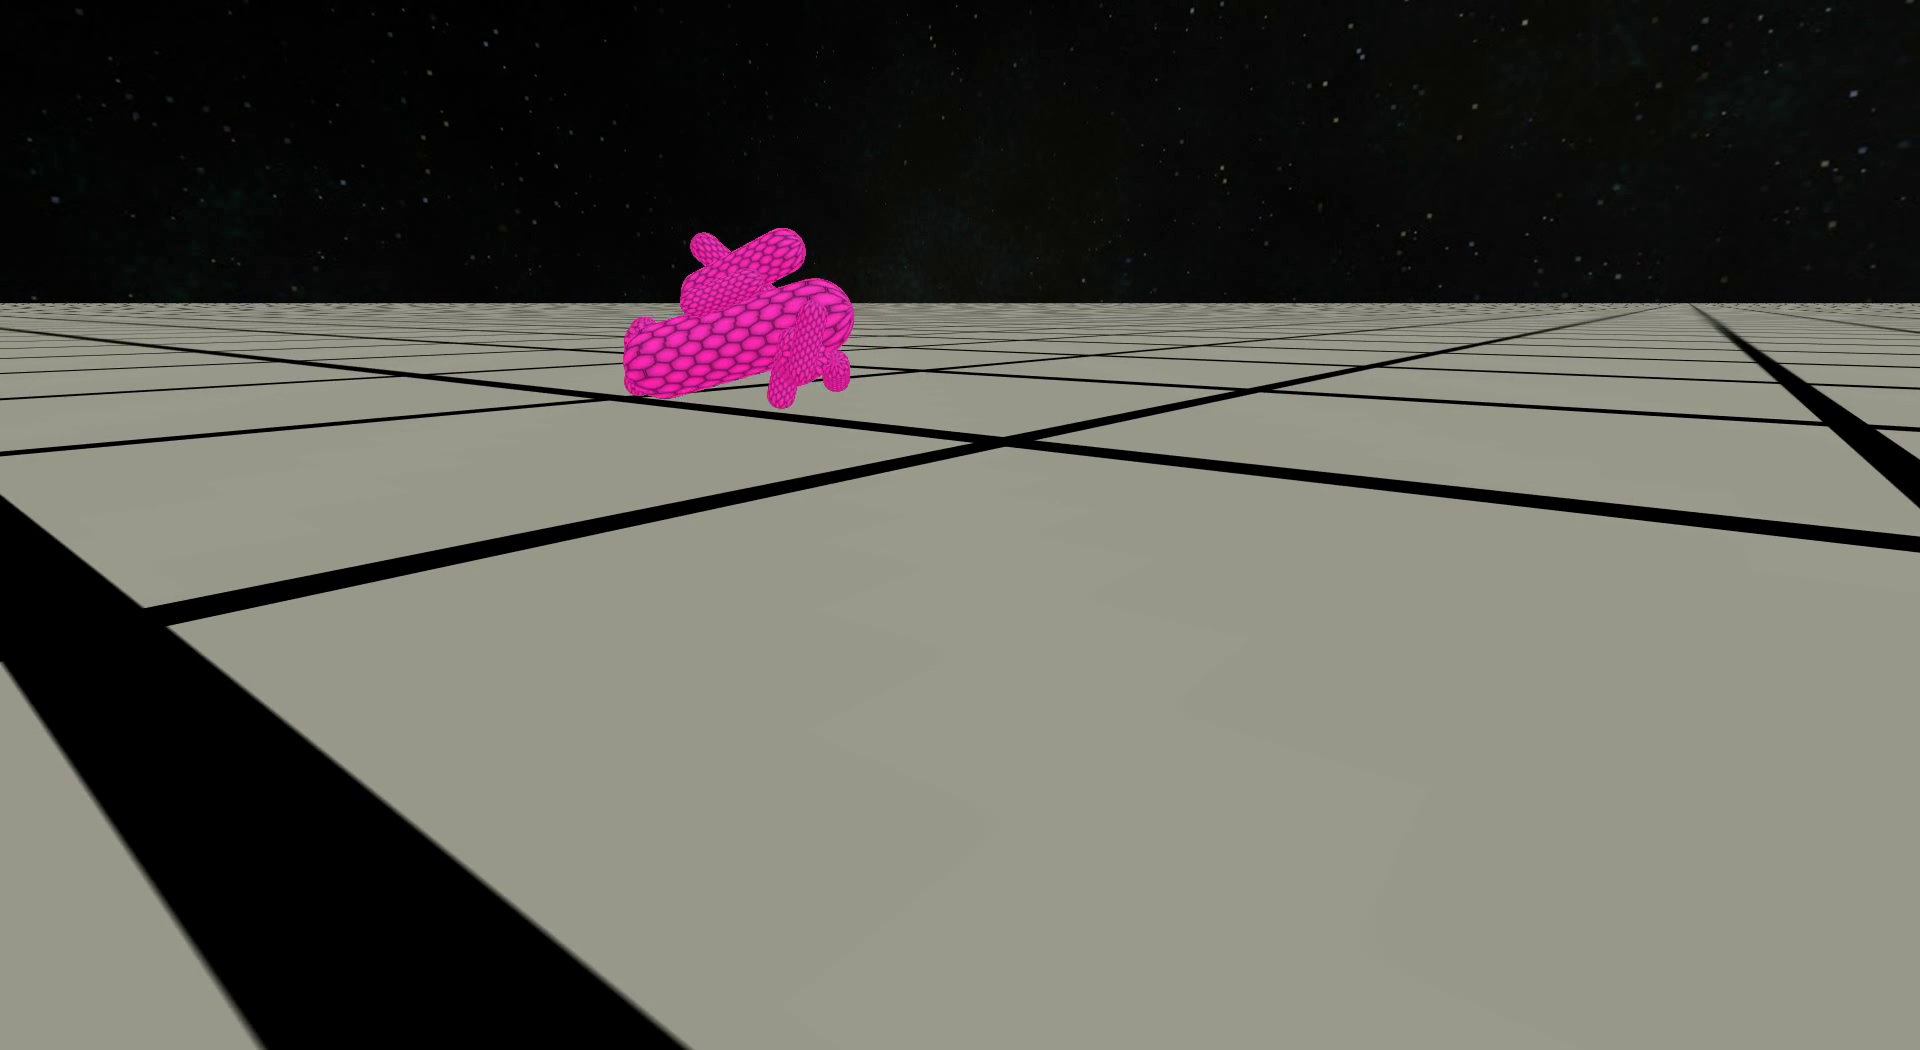
\includegraphics[width=0.45\textwidth]{results/evolved-creatures/sine/jumper2/373.png}
%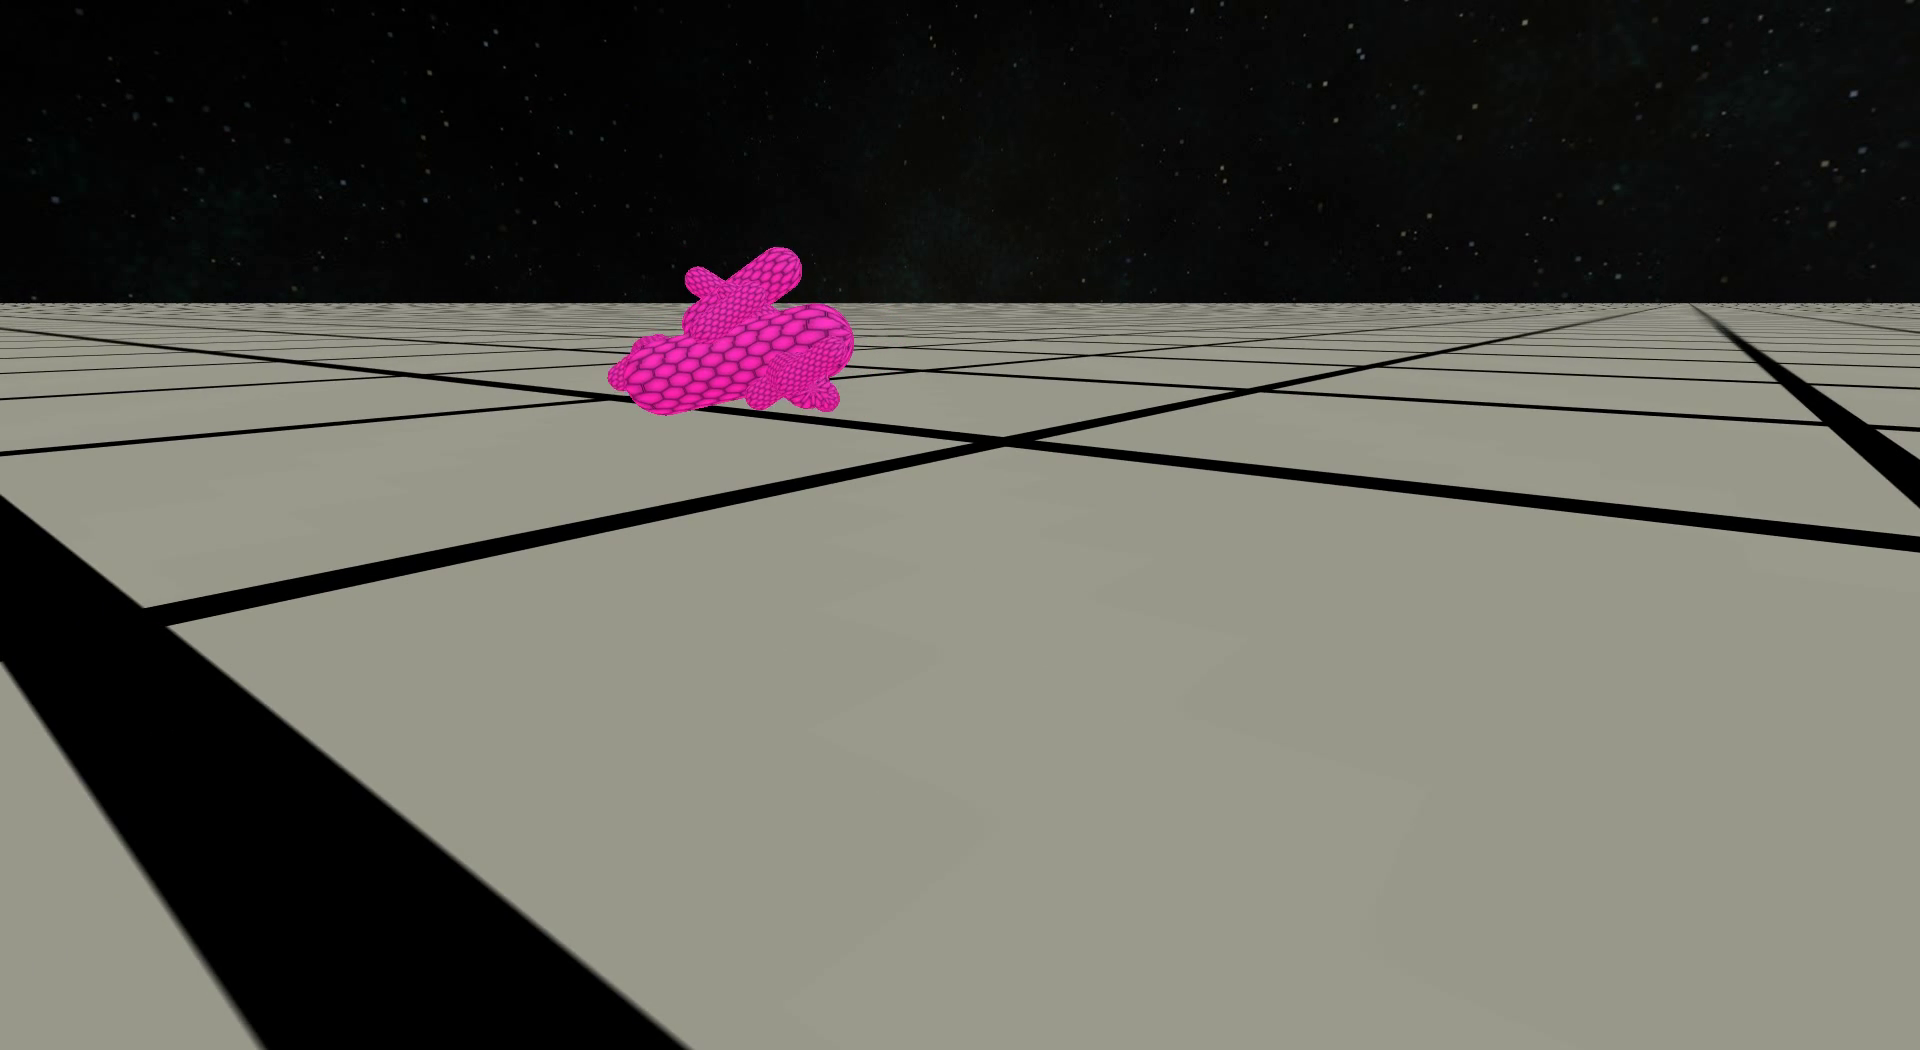
\includegraphics[width=0.45\textwidth]{results/evolved-creatures/sine/jumper2/406.png}
\caption[Figure of another jumper using sinusoidal controllers.]{Figure of another jumper using sinusoidal controllers. Its two legs in the back propulse the body forward while the front contact point acts as a stabilization. A video of the jumping creature can be found on YouTube: \url{https://youtu.be/xc9uWrDYRic}.}
\label{figure:successfulcreatures-jumper2}
\end{figure}

\begin{figure}[tb]
\centering
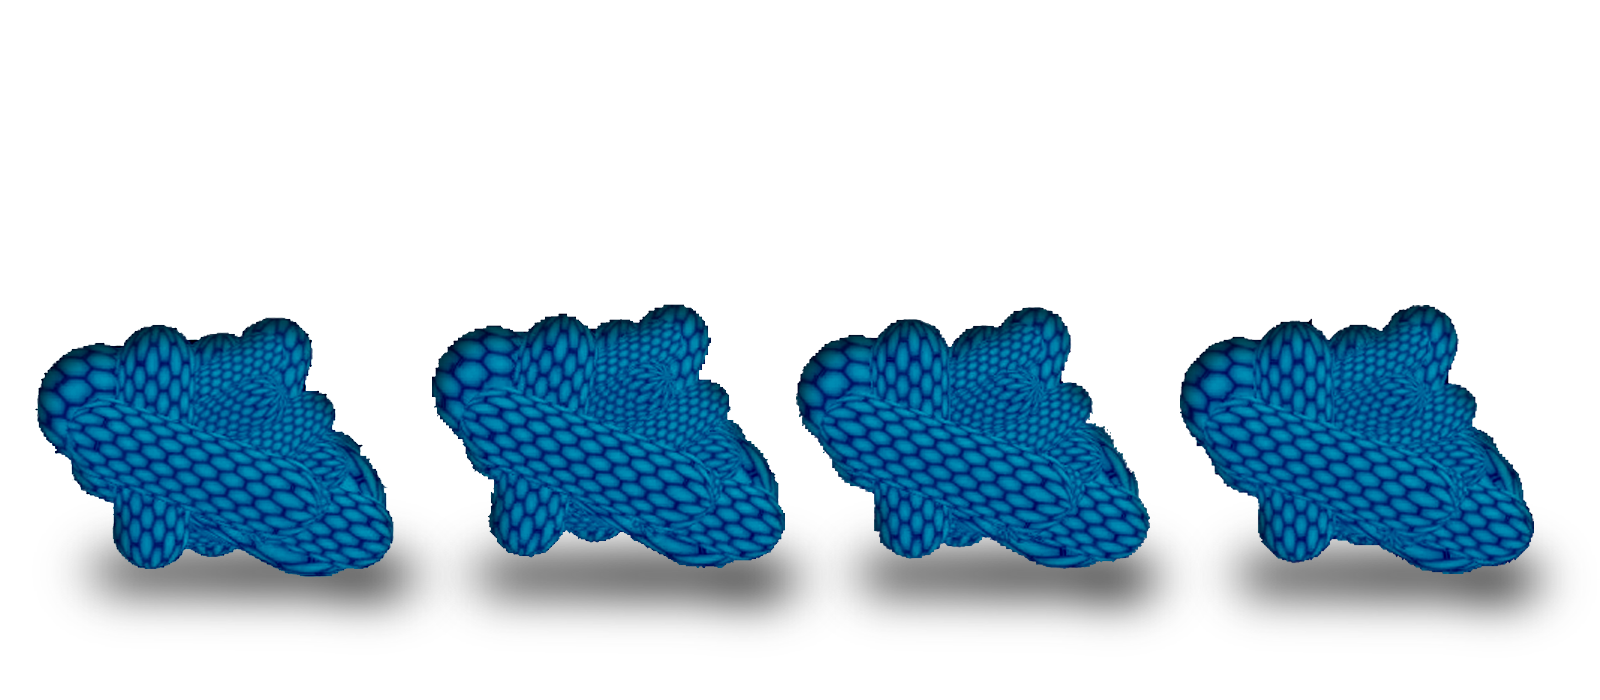
\includegraphics[width=0.85\textwidth]{results/evolved-creatures/sine/walker1/walker1-animation.png}
%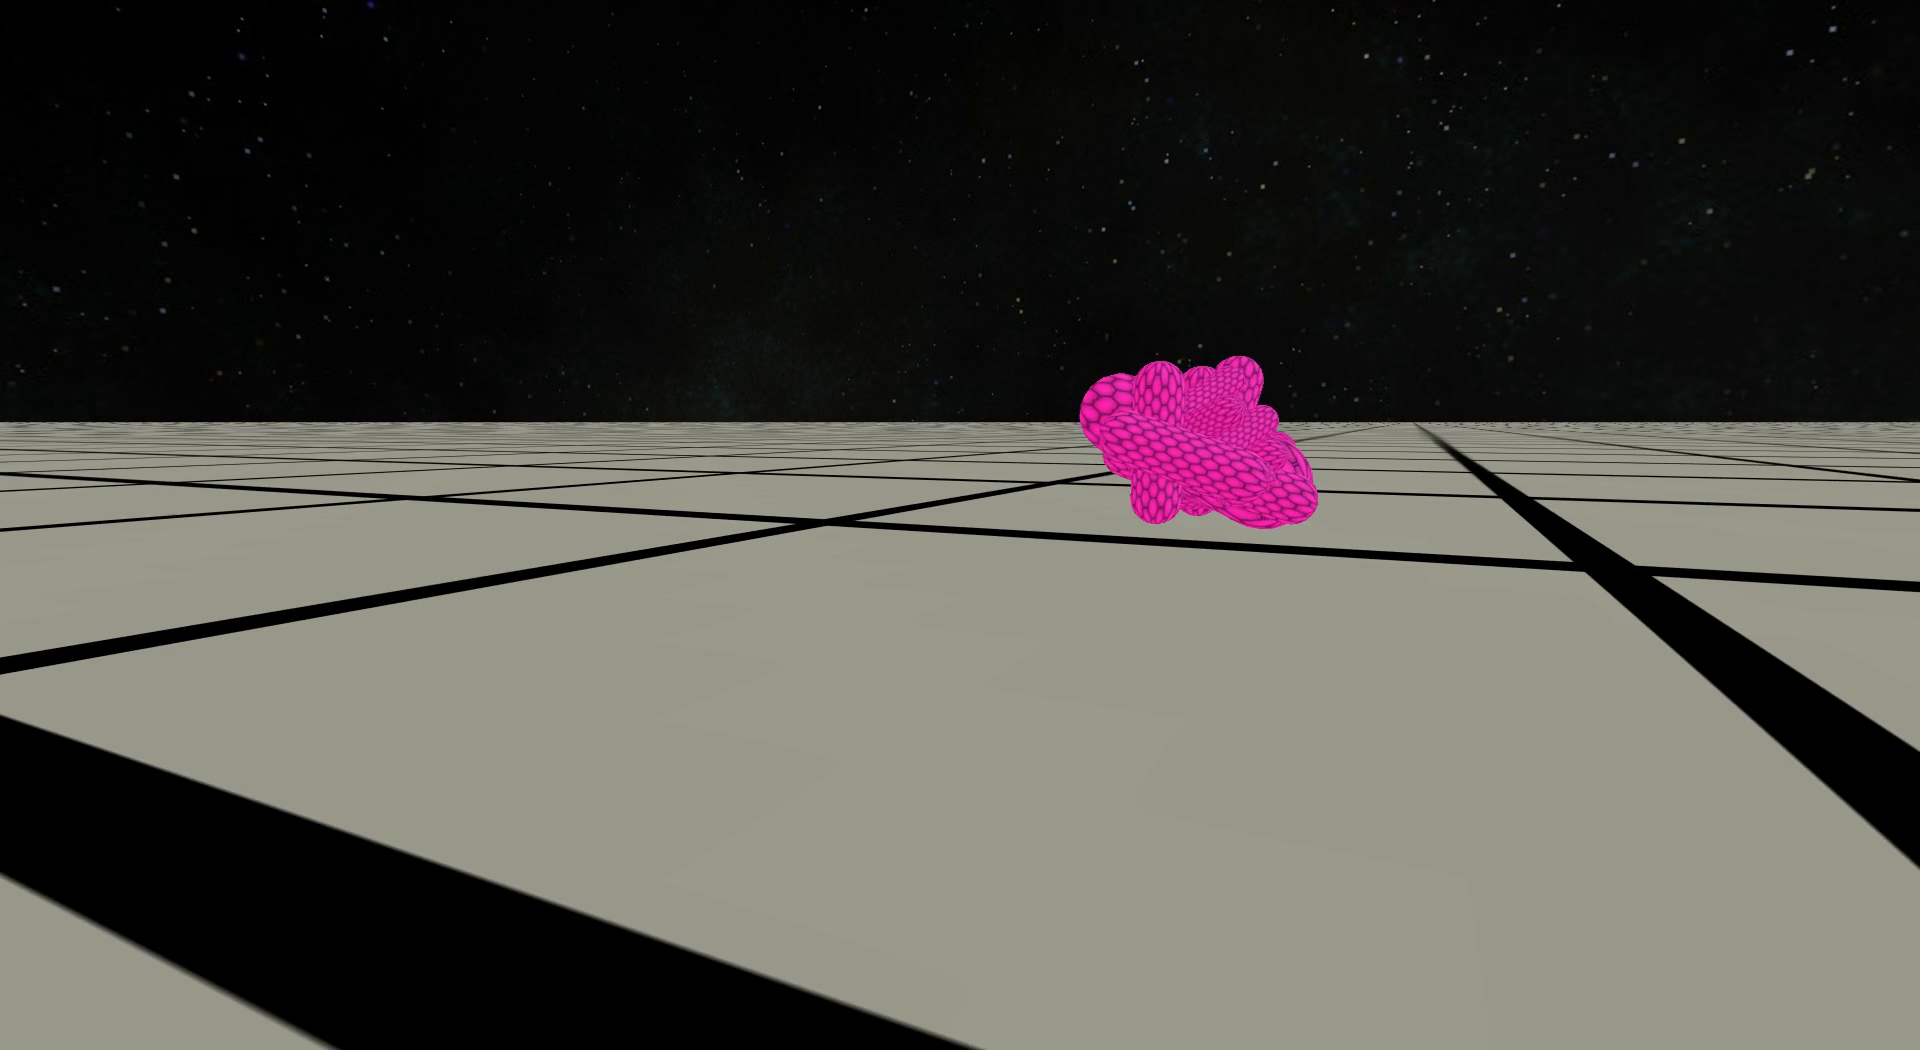
\includegraphics[width=0.45\textwidth]{results/evolved-creatures/sine/walker1/447.png}
%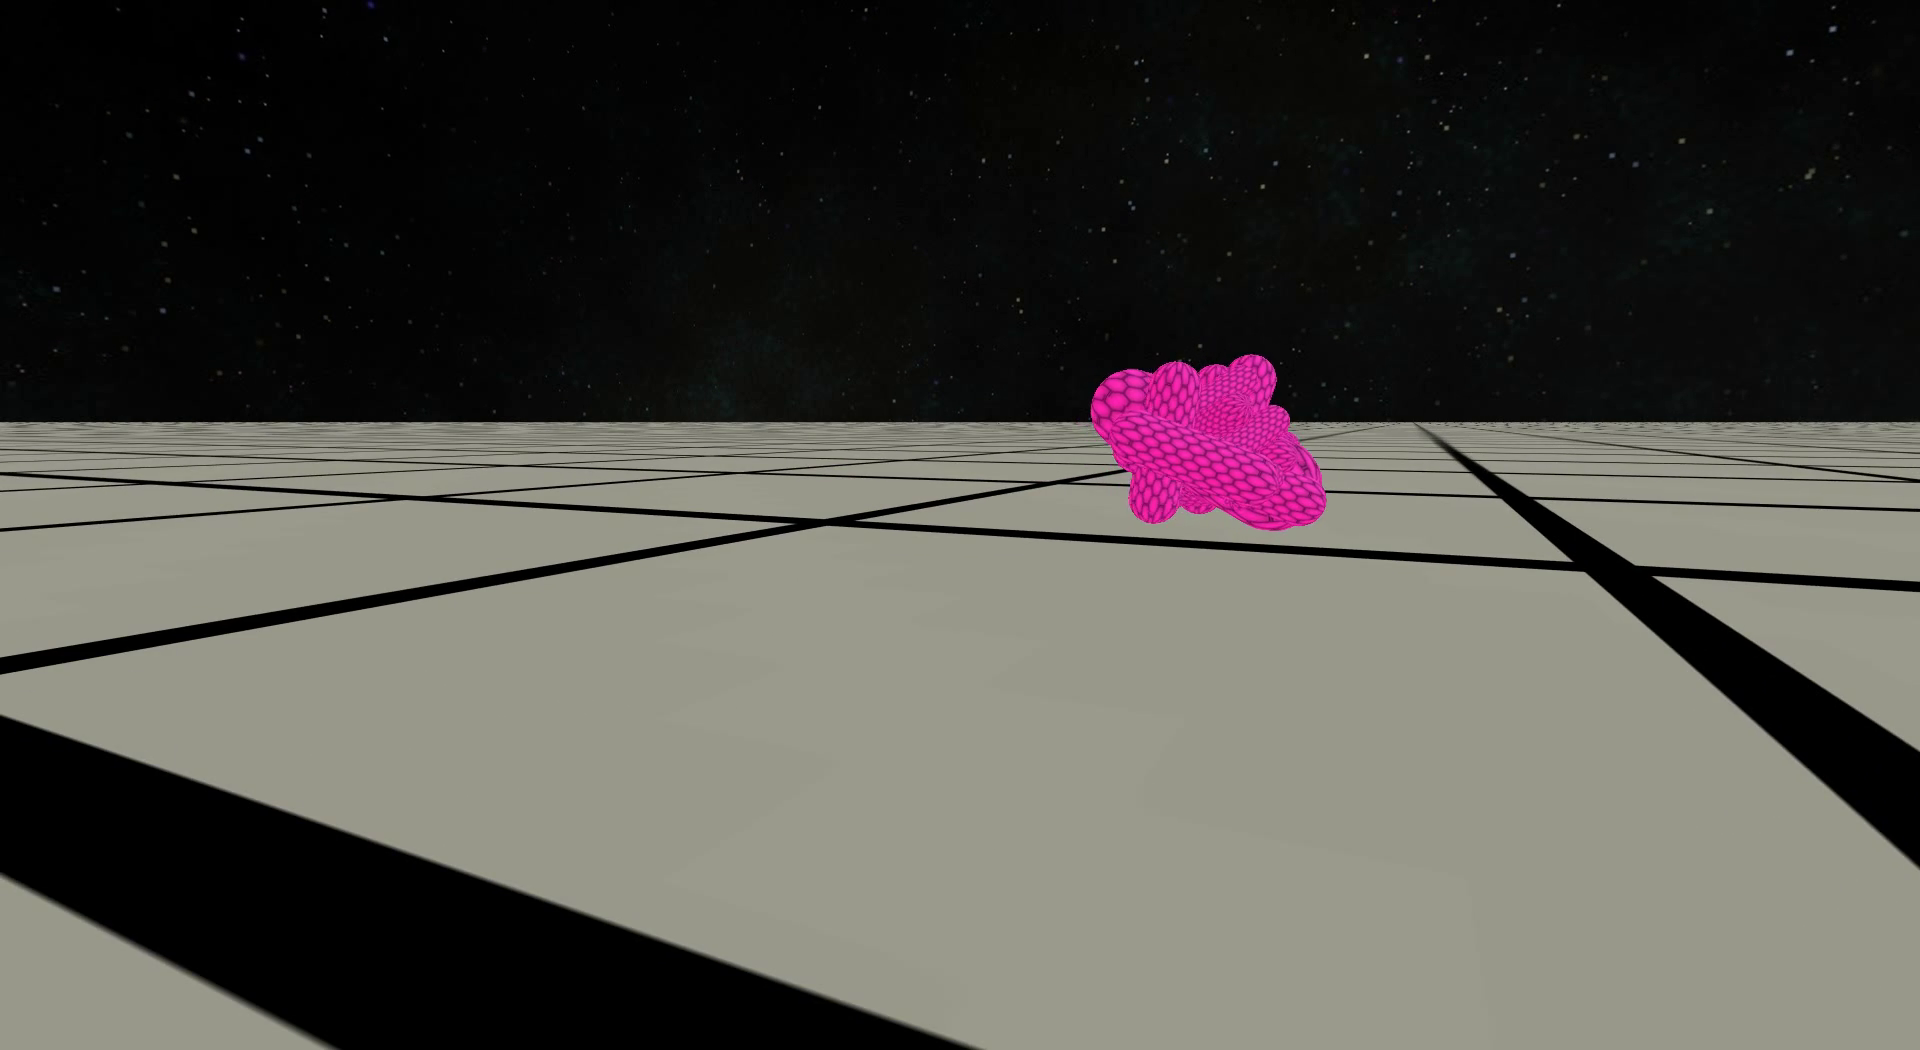
\includegraphics[width=0.45\textwidth]{results/evolved-creatures/sine/walker1/460.png}
%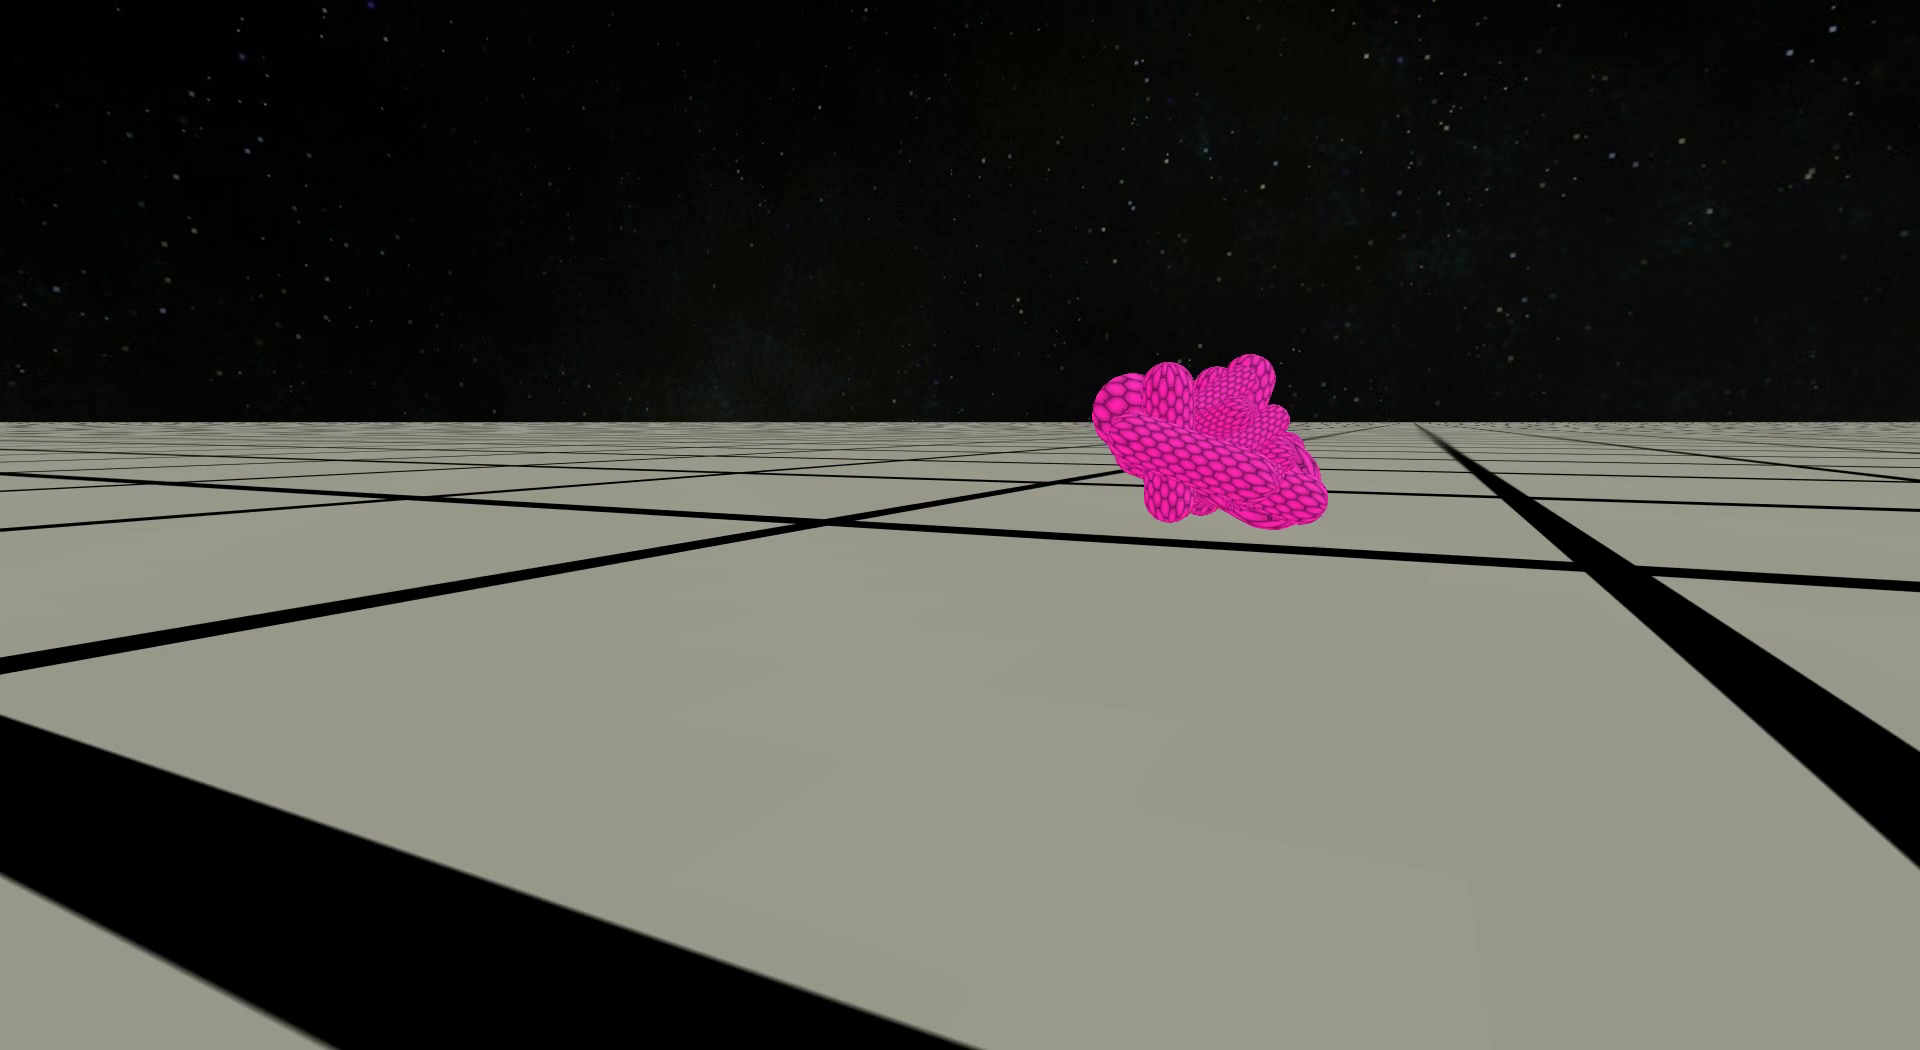
\includegraphics[width=0.45\textwidth]{results/evolved-creatures/sine/walker1/468.png}
%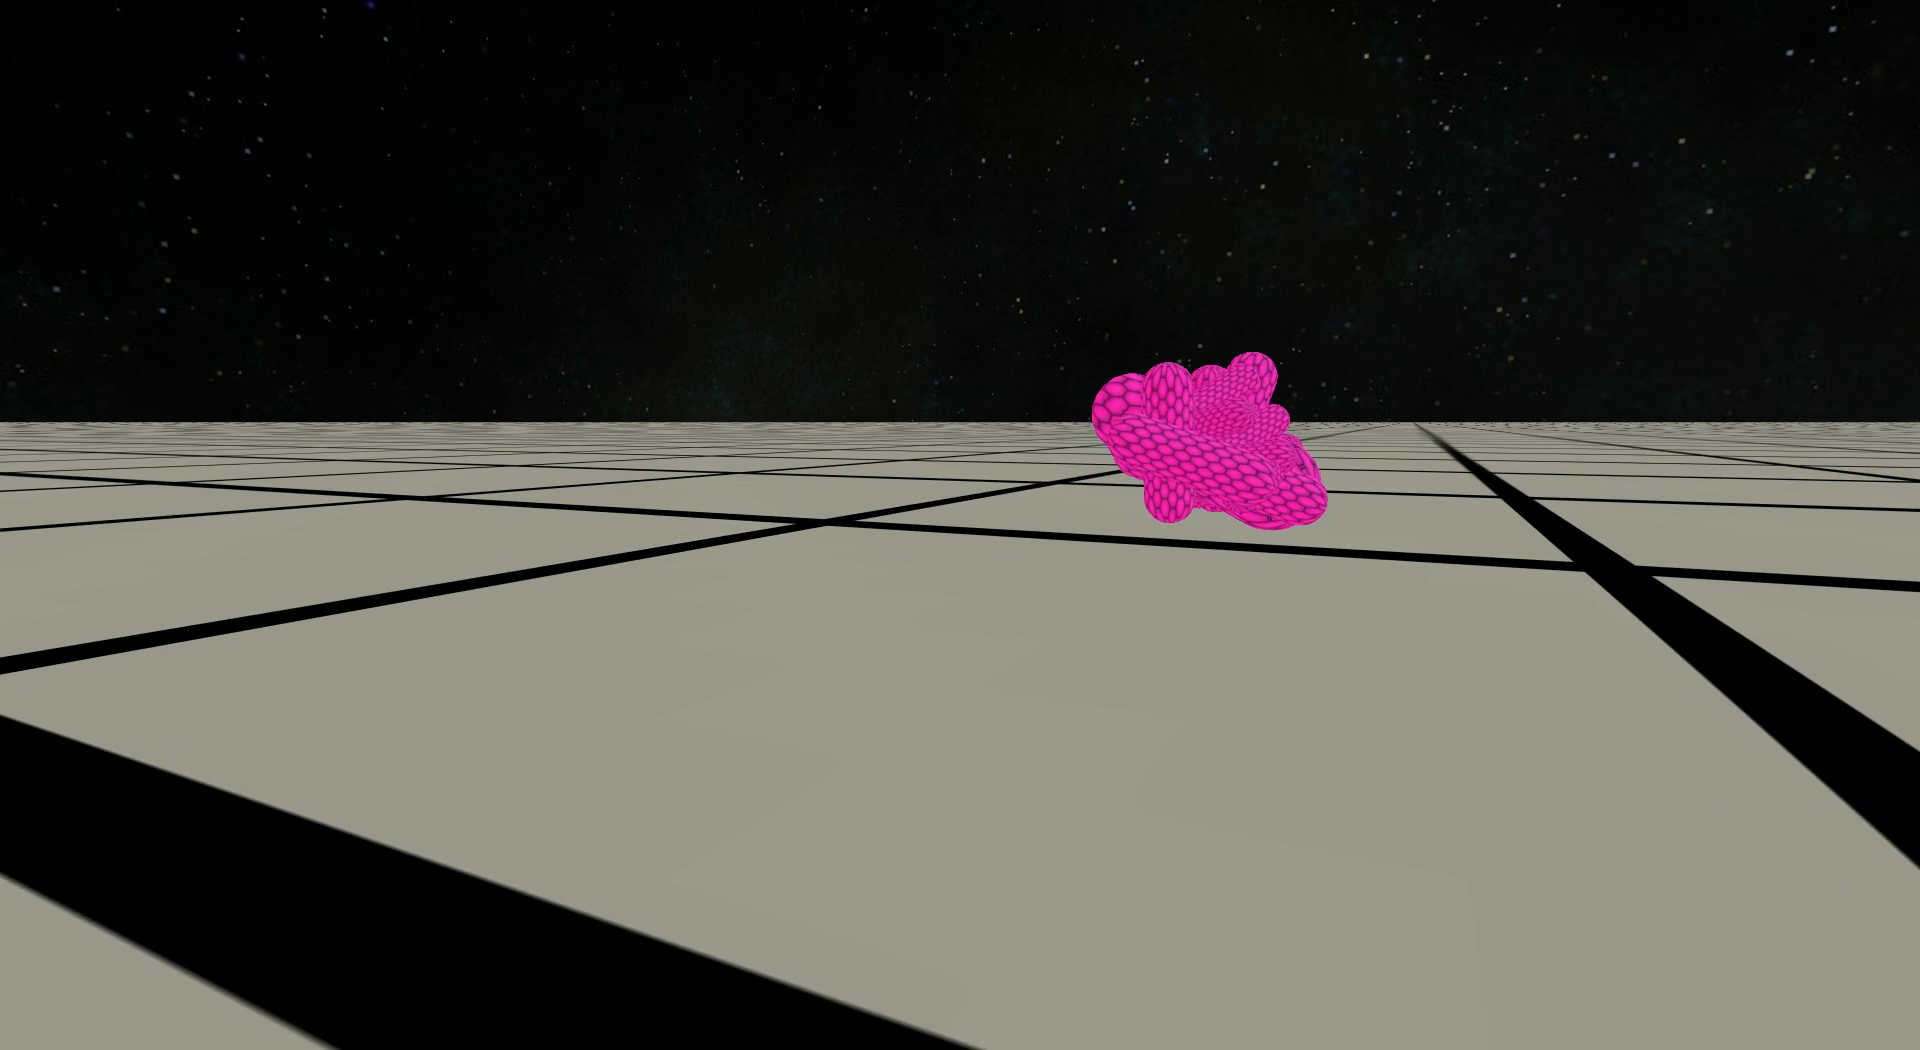
\includegraphics[width=0.45\textwidth]{results/evolved-creatures/sine/walker1/471.png}
\caption[Figure of a walker using sinusoidal controllers.]{Figure of a walker using sinusoidal controllers. It has two legs in the back, which push the body forward. The front contact point again stabilizes the movement. A video of the walking creature can be found on YouTube: \url{https://youtu.be/PYMajm8A9eQ}.}
\label{figure:successfulcreatures-walker1}
\end{figure}

\begin{figure}[tb]
\centering
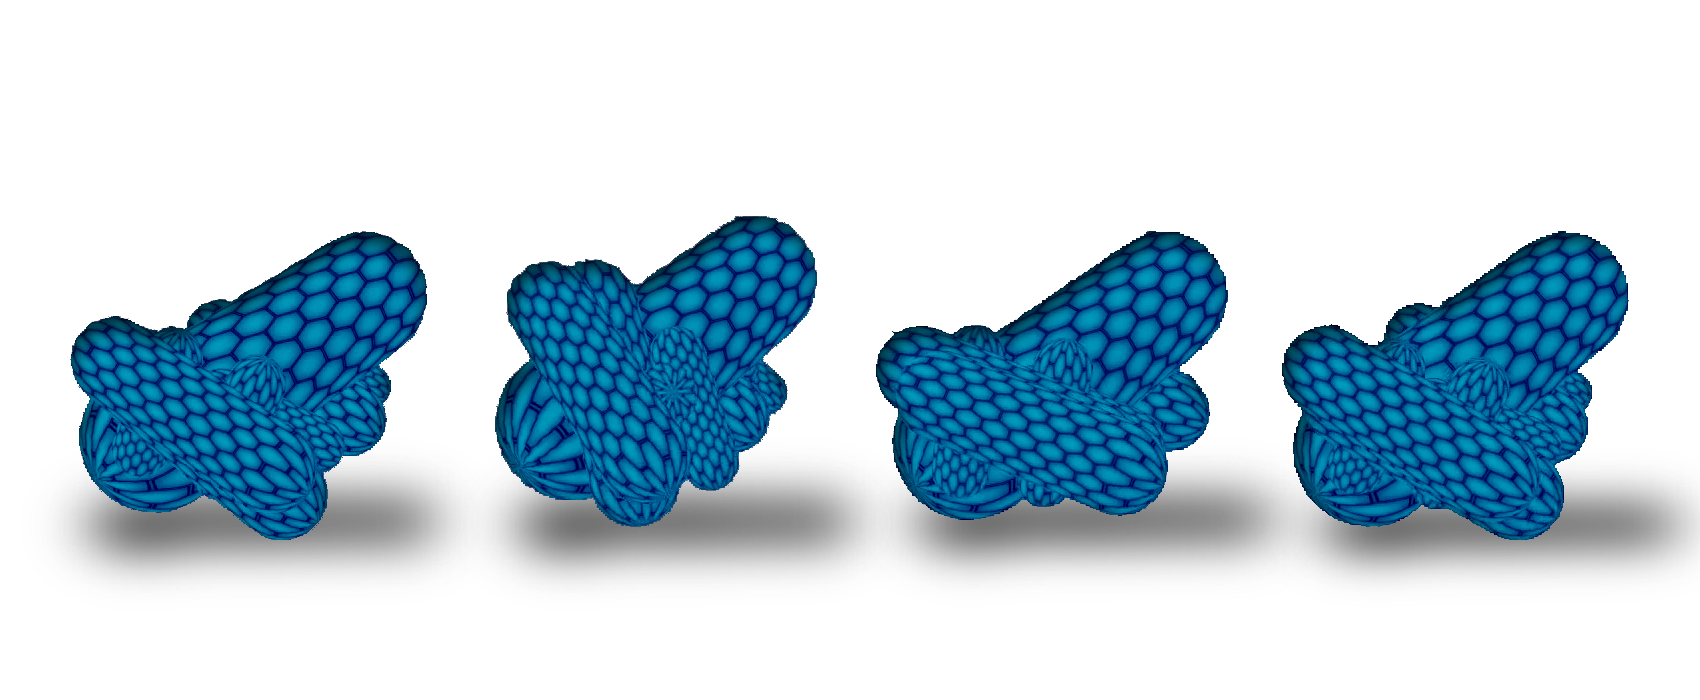
\includegraphics[width=0.9\textwidth]{results/evolved-creatures/sine/walker2/walker2-animation.png}
%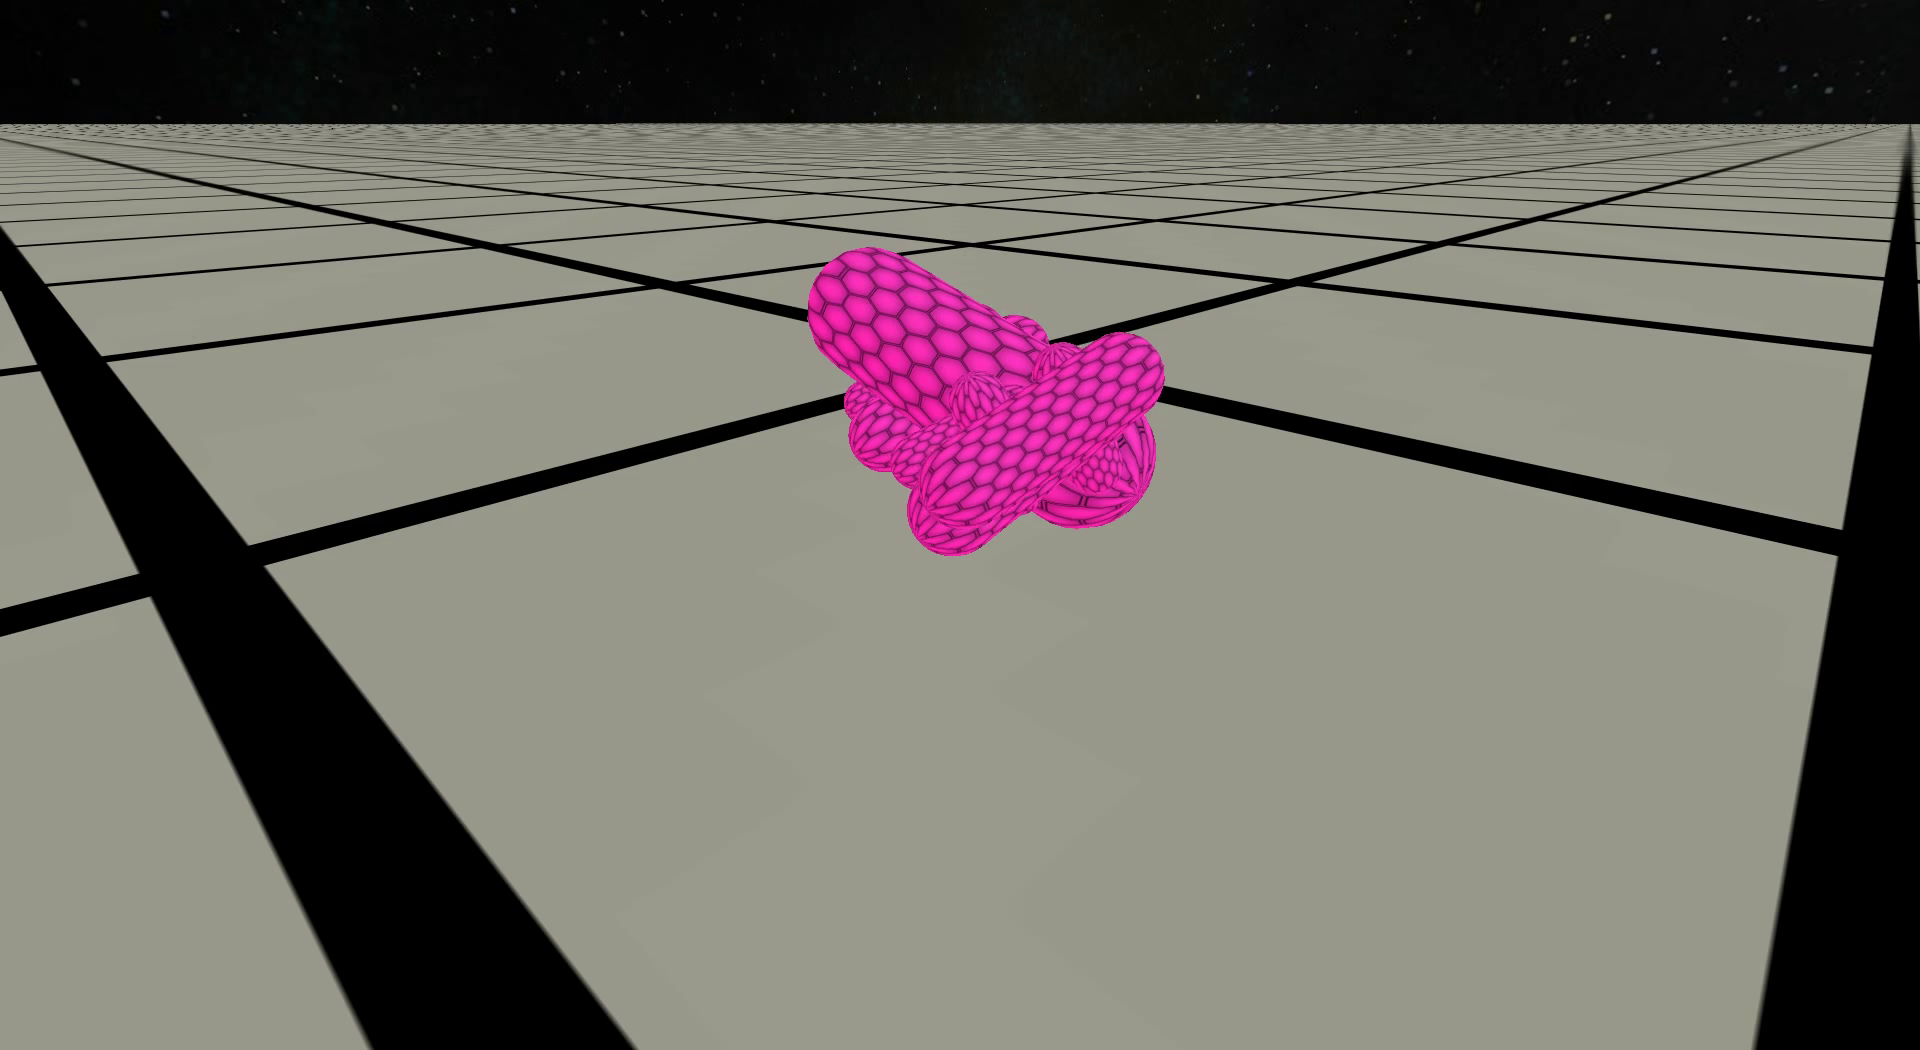
\includegraphics[width=0.45\textwidth]{results/evolved-creatures/sine/walker2/027.png}
%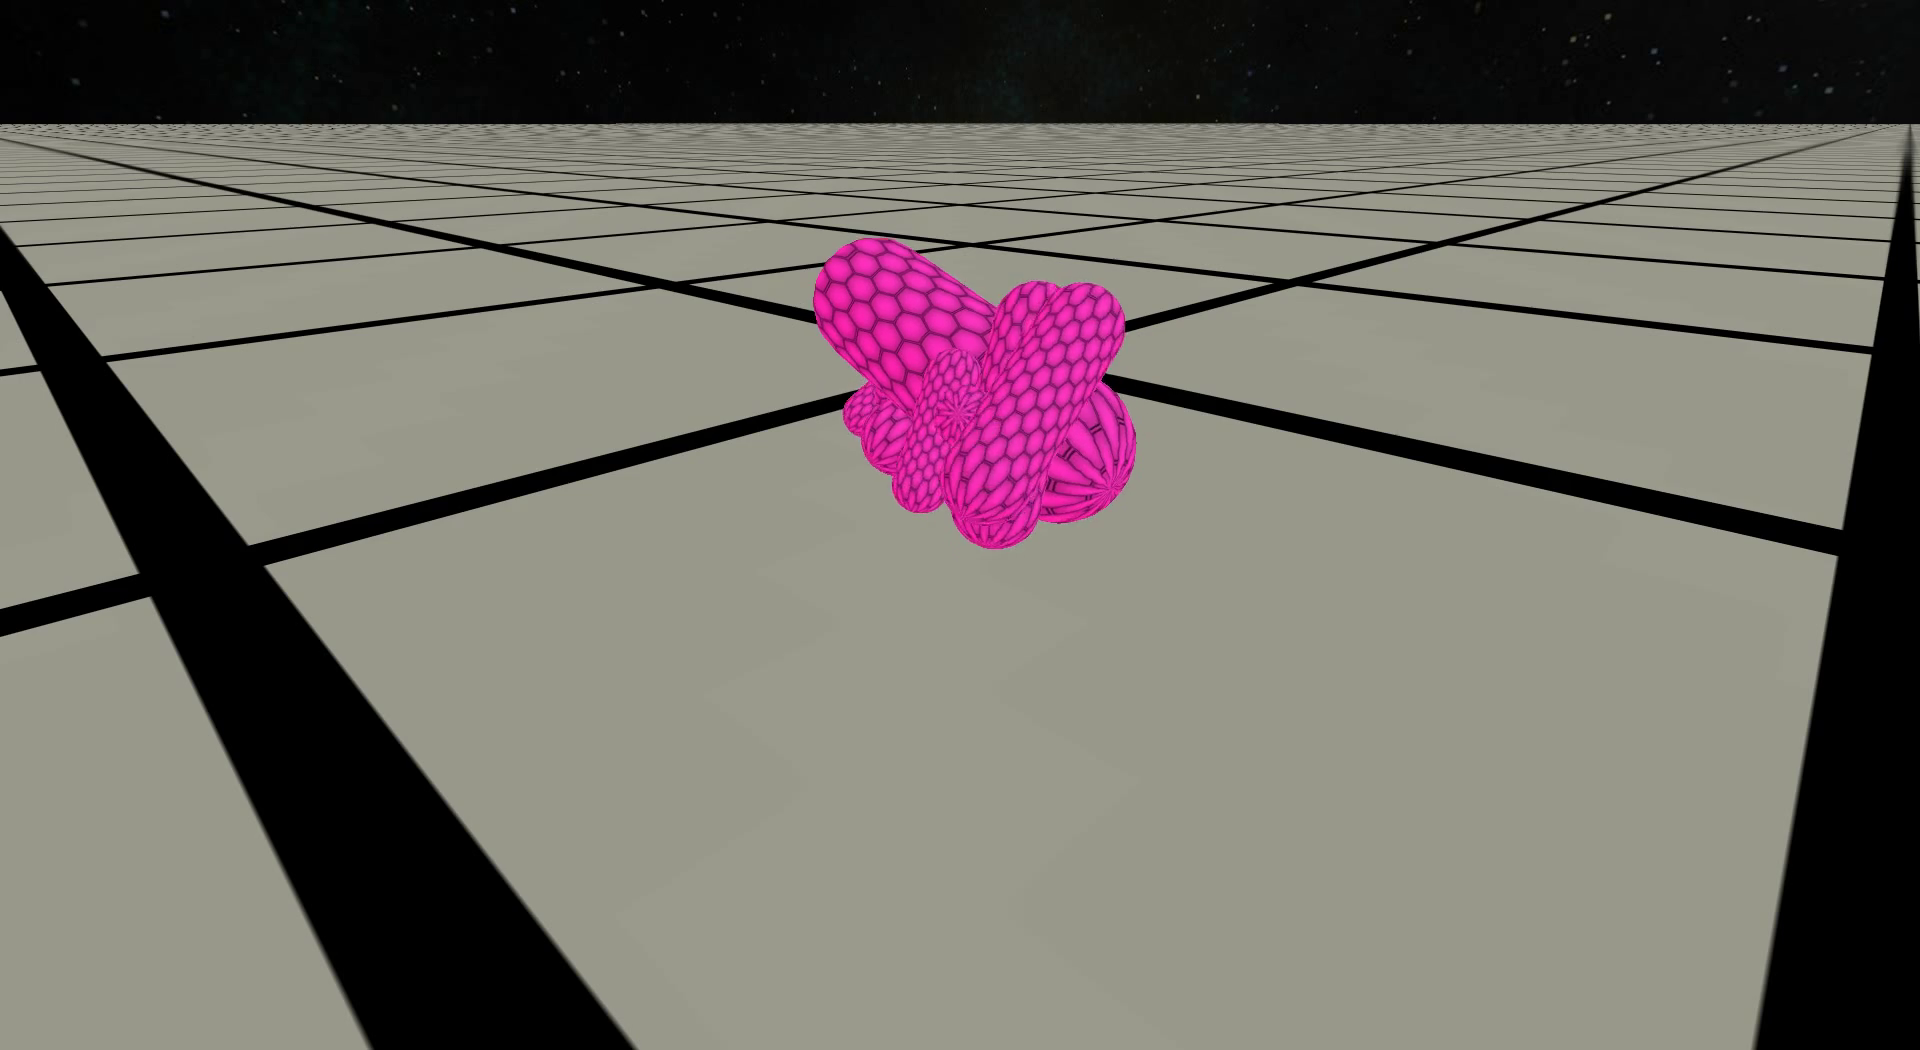
\includegraphics[width=0.45\textwidth]{results/evolved-creatures/sine/walker2/048.png}
%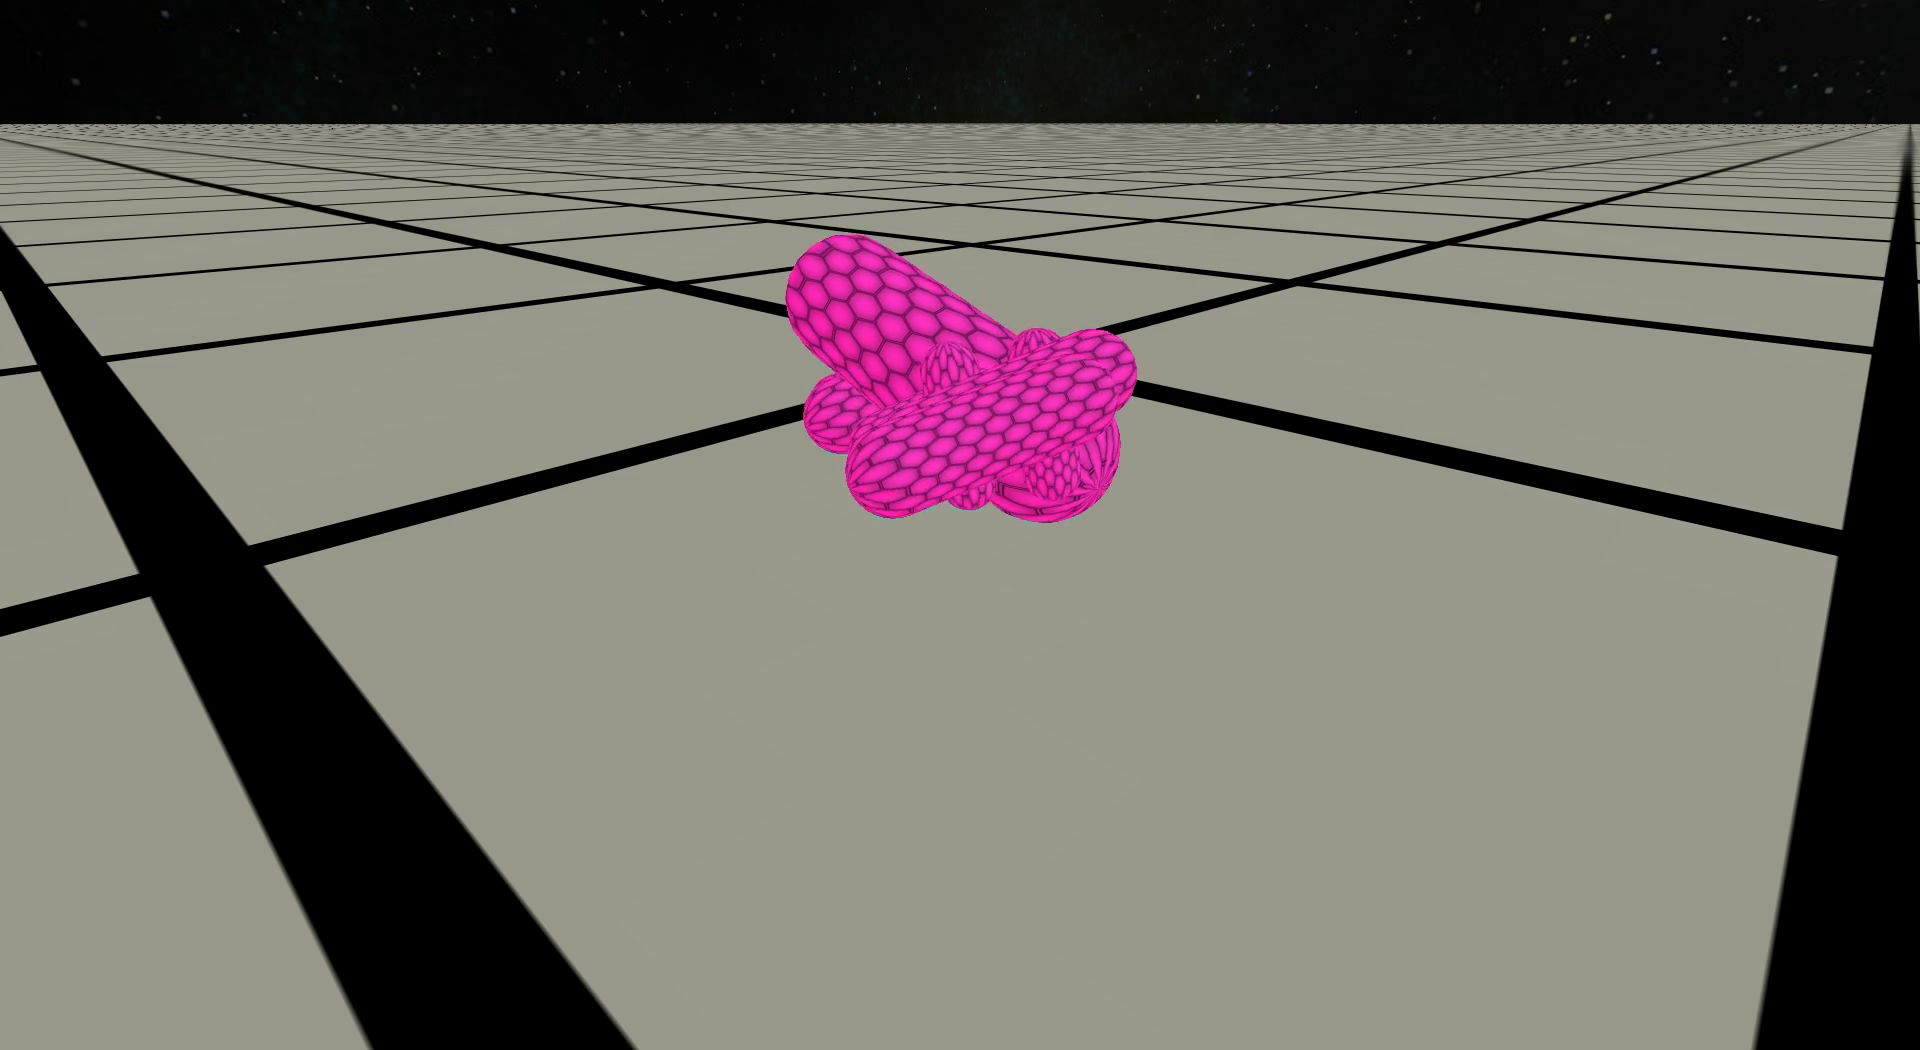
\includegraphics[width=0.45\textwidth]{results/evolved-creatures/sine/walker2/064.png}
%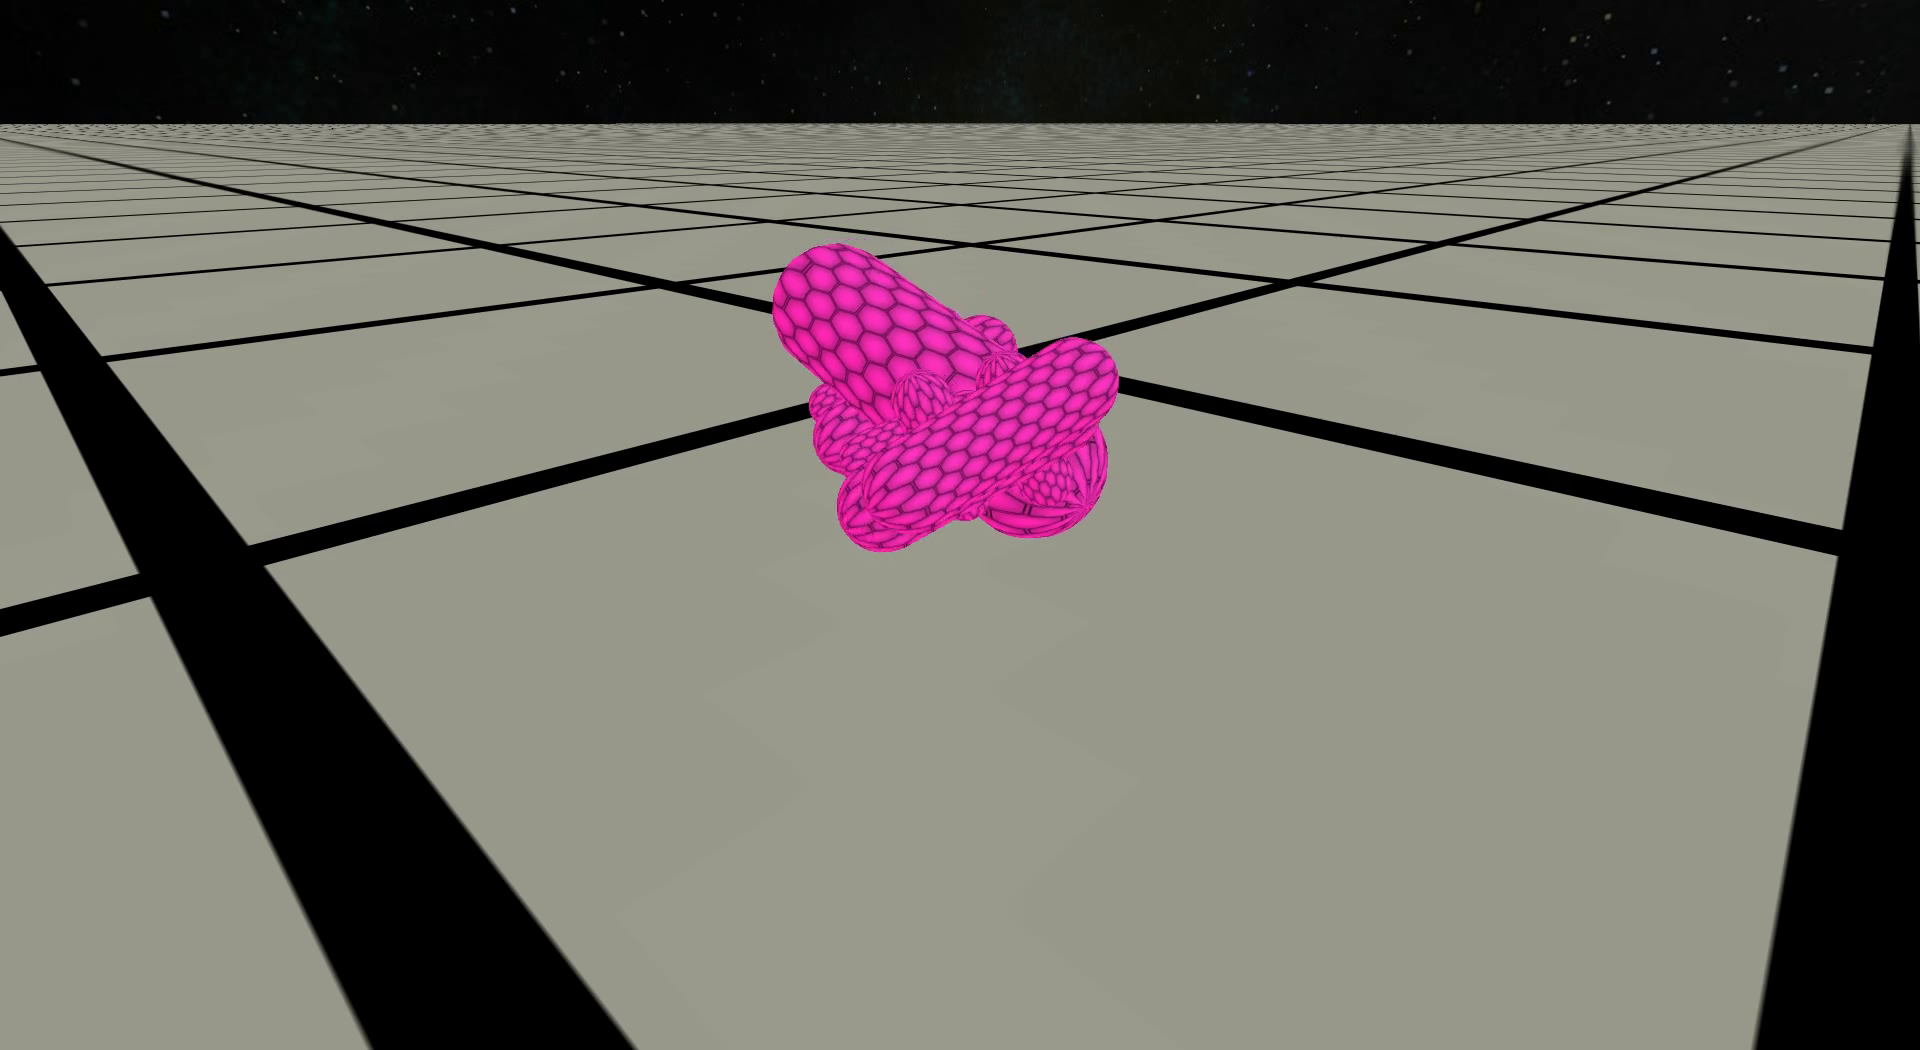
\includegraphics[width=0.45\textwidth]{results/evolved-creatures/sine/walker2/079.png}
\caption[Figure of another walker using sinusoidal controllers.]{Figure of another walker using sinusoidal controllers. This creature has many legs on both sides, which synchronously touch the ground and make the body crawl forward. A video of the walking creature can be found on YouTube: \url{https://youtu.be/OAmdOUpvuPY}.}
\label{figure:successfulcreatures-walker2}
\end{figure}

Creatures that exhibit successful locomotion seem to share a common ancestor, which might have been the first creature to evolve a successful walking pattern, since all of its offspring share a similar skin coloring. %
%
Since the skin color is randomly set for one body part, the common ancestor could only have had all the same color and must have been replicated using crossover. %
%
In crossover (as described in \ref{subsec:crossover}), subsections of the two participating creature genotypes are taken and combined into one new genotype. %
%
This process involves no mutations, therefore the crossover must have happened mainly among creatures sharing the same skin coloring. %
%
The elitism mechanism of the evolutionary process, passing the most successful creatures directly to the next generation, kept the first successful creature, that then generated an onset of an avalanche of successful creatures, flooding the population with very similar solutions. 

The major drawback of the sinusoidal oscillator controller is that they do not show any adaption during the evaluation depending on the environment. %
%
The only way for the controller to adapt is on the evolutionary time-scale through mutation, which does not result in an advantage for the individual in its current evaluation, but only helps a future generation of the individual to eventually converge to a new, applicable solution. 

\section{Simple Limiter Control in the Simulator}
% rev. 3

The chaotic controller, introduced in the previous chapter, which uses an underlying chaotic system, is a marvellous source of periodic patterns of motion due to its infinite number of unstable periodic orbits. %
%
If a creature could use simple limiter control to stabilize UPOs and exploit the periodic orbits for locomotion patterns, this could lead to a more robust and adaptive way of motion. %
%
Experimentally, this would mean that if the creatures exhibited periodic locomotion patterns, it could be shown that the successful creatures controlled the amount of chaotic movement of the controller or the chaotic movement of the body part and stabilized unstable periodic orbits to exploit it for body part motion. %
%
Showing that the controller or body part motion is less chaotic can be shown by calculating the largest Lyapunov exponent, which accounts for the amount of divergence of two slightly different initial conditions of the controller or the body part motion.

The experiments were run on the chaotic controller as described in \ref{subsec:chua-circuit}. %
%
Simple limiters can come in various ways, since they only must be natural to the system at hand \cite{bib:Corron2000}. %
%
Therefore the first experiments were run using chaotic controllers without direct limiters implemented into the controllers. %
%
The second experiments then used sensory feedback to impose limiters on the chaotic controller. 

\subsection{Indirect Limiter Control through the Morphology}
% rev. 3

\begin{figure}[H]
%\hspace*{-4.2in}
\begin{tikzpicture}
% classes
\tikzstyle{root} = [draw=black!80, thick,minimum width=1.5cm,minimum height=1cm, circle, fill=black!20]
\tikzstyle{class1} = [minimum width=3cm, minimum height=2cm,draw=black!80, thick, fill=blue!5, rounded corners, rectangle]
\tikzstyle{class2} = [minimum width=2.5cm,minimum height=0.2cm, rounded corners,rectangle, fill=orange!80]
\tikzstyle{class3} = [minimum width=2.5cm,minimum height=0.2cm, rounded corners,rectangle, fill=red!80]

%###############################################
% external output
%###############################################

%###############################################
% internal controller state
%###############################################

%###############################################
% controller symbol
%###############################################

%###############################################
%  force control
%###############################################

%###############################################
% joint state
%###############################################

%###############################################
% joint limits
%###############################################

%###############################################
% joint damping
%###############################################

%###############################################
% joint symbol
%###############################################



\end{tikzpicture}


\caption[The indirectly limited chaotic controller and joint complex]{The indirectly limited chaotic controller and its interaction with the joint. The limiters defined through the environment and the joint properties constrain only the movement of the joint, but do not influence the chaotic controller behavior itself. Therefore the environmental influences and the joint properties can not change the dynamics of the controller.}
\label{figure:indirect-limit-controller-joint-complex}
\end{figure}

The first experiments use chaotic controllers without direct limiters. %
%
The controllers start with different initial conditions and different integration speeds, but are not limited using sensory input. %
%
Therefore the chaotic trajectories emitted from the controllers are only limited through the morphology. %
%

In the following plot (Figure \ref{figure:unlimited-model-leg}), the behavior of the model leg with an unlimited controller can be observed. %
%
The model leg continuously rotates into one direction until it hits the joint limit, from which it then moves back and forth in the case the controller signal's sign changes for a short time. %
%
However no periodic movement can be observed over the long run. %

\begin{figure}[H]
	\centering
	\begin{minipage}{1.3\textwidth}
	\hspace*{-5em}
	\begin{tikzpicture}

% classes
\pgfdeclarelayer{background}
\pgfdeclarelayer{foreground}
\pgfsetlayers{background,main,foreground}
\tikzstyle{bigbox} = [draw=black!80, thick, fill=black!5, rounded corners, rectangle]
\tikzstyle{box} = [minimum size=0.6cm, rounded corners,rectangle, fill=black!50]

\node[align=left] at (0,0){\underline{Controller State Space}};
\node[inner sep=0pt] (controller-state-space) at (0,-3)
{
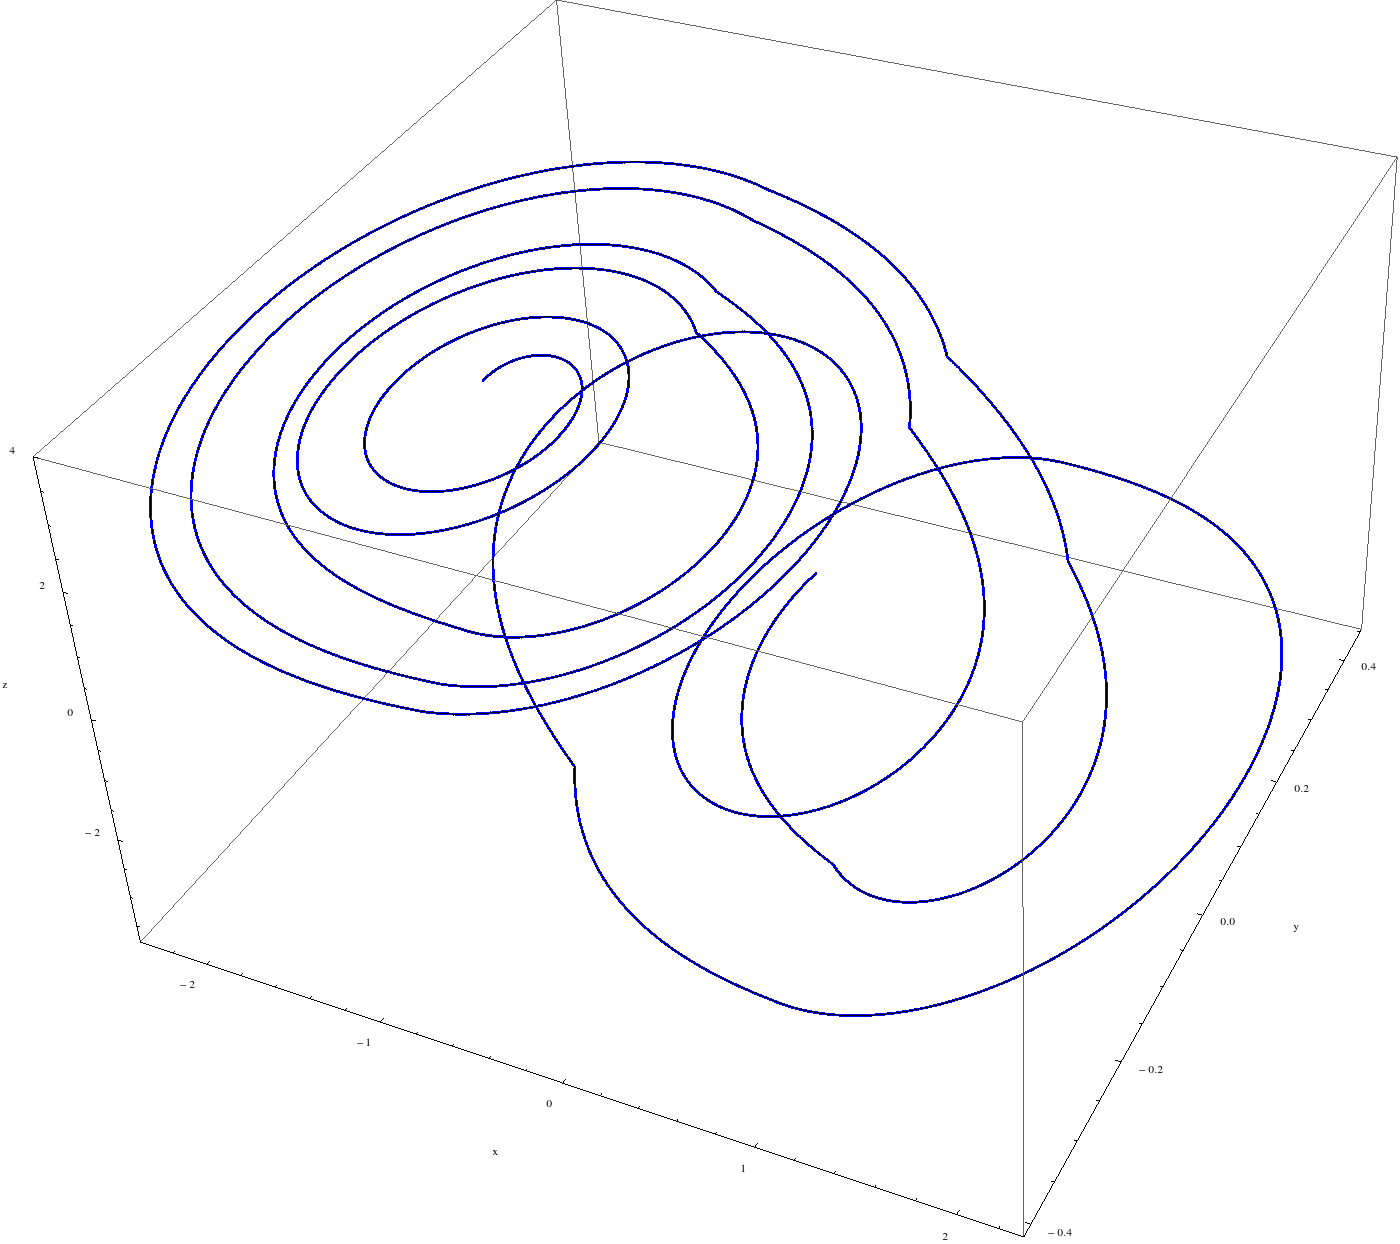
\includegraphics[width=0.45\textwidth]{model-organisms/model-leg/Modelleg-0g-100s-friction00-force0-7-damping0-05-(x)(-1-5)(y)z.png}
};

\node[align=left] at (9,0){\underline{Joint Dynamics}};
\node[inner sep=0pt] (joint-dynamics) at (9,-3)
{
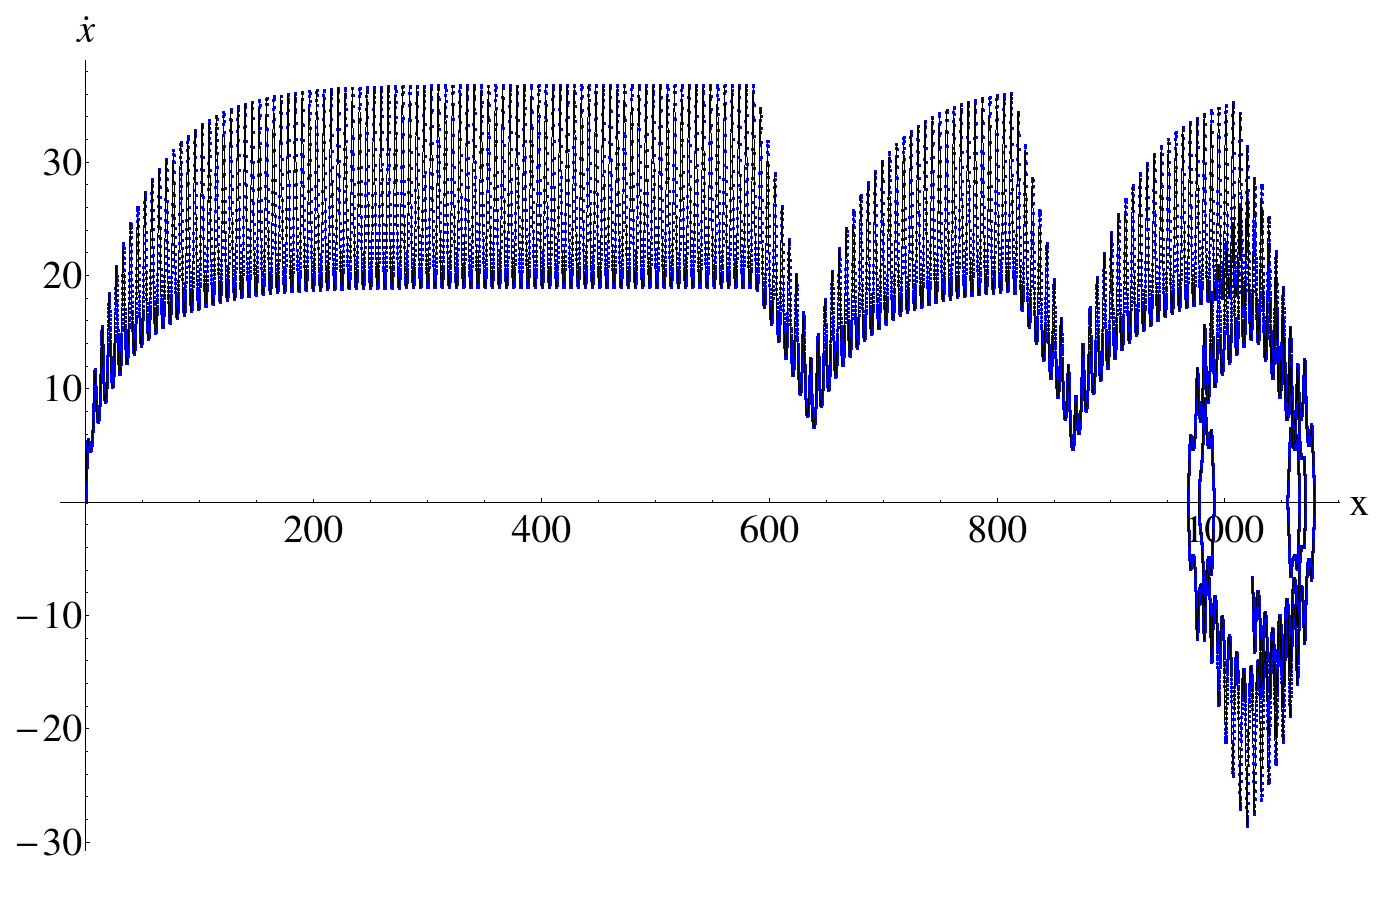
\includegraphics[width=0.45\textwidth]{model-organisms/model-leg/Modelleg-0g-100s-friction00-force0-7-damping0-05-(x)(-1-5)(y)z-joint.png}
};
	\end{tikzpicture}
	\end{minipage}
	\caption[Unlimited chaotic controller controlling model leg.]{Unlimited chaotic controller controlling model leg. The velocity on the y axis fluctuates in the positive range and therefore, the position increases positively. At the end, the velocity switches from positive to negative, making the position oscillate as well. However, as the chaotic trajectory again switches to another limit cycle, the position increases again only into one direction.}
	\begin{tabular}{l|ll}
	\hline 
	Gravity: 0g  & Sensors: & - \\
	 Output: z(t) \(\rightarrow\) Joint torque & & - \\
	  Torque scaling curve: \(0.7~(mass_1~\cdot~mass_2)\) & & - \\
	  \hline
	\end{tabular}

	\label{figure:unlimited-model-leg}
\end{figure}

Since the model leg might be a bad predictor of how higher complexity could influence the resulting creature, 4 different evolutionary settings in terms of evaluation time and number of creatures in the population were run. %
%
However, the desired limiter control exhibiting periodic or quasi-periodic motion could not be observed in any of the creatures. %
%
This could be explained due to the lacking feedback from the body part to the chaotic system itself. %
%
That is why the chaotic system runs completely uninfluenced and is independent of the body part being limited in its movement. %
%
Therefore it was necessary to implement sensory feedback of the respective, controlled joint so that the limits of the morphology would impose limiters on the chaotic controller.

\subsection{Direct Limiter Control through Sensory Feedback}
% rev. 2

\begin{figure}[H]
%\hspace*{-1.2in}
% Define a variable as a length
% Input:
%   #1 Variable name
%   #2 Value
%
% Example:
%   \nvar{\varx}{2cm}
\newcommand{\nvar}[2]{%
    \newlength{#1}
    \setlength{#1}{#2}
}

% Define a few constants for drawing
\let\dg\relax
\let\ddx\relax
\nvar{\dg}{0.3cm}
\def\dw{0.25}\def\dh{0.5}
\nvar{\ddx}{1.2cm}

% Define commands for links, joints and such
\def\link{\draw [double distance=1.5mm, very thick] (0,0)--}
\def\joint{%
    \filldraw [fill=white] (0,0) circle (5pt);
    \fill[black] circle (2pt);
}
\def\grip{%
    \draw[ultra thick](0cm,\dg)--(0cm,-\dg);
    \fill (0cm, 0.5\dg)+(0cm,1.5pt) -- +(0.6\dg,0cm) -- +(0pt,-1.5pt);
    \fill (0cm, -0.5\dg)+(0cm,1.5pt) -- +(0.6\dg,0cm) -- +(0pt,-1.5pt);
}
\def\robotbase{%
    \draw[rounded corners=8pt] (-\dw,-\dh)-- (-\dw, 0) --
        (0,\dh)--(\dw,0)--(\dw,-\dh);
    \draw (-0.5,-\dh)-- (0.5,-\dh);
    \fill[pattern=north east lines] (-0.5,-1) rectangle (0.5,-\dh);
}

\def\dampattach{12pt}
\def\jointsurf{0.7mm}
\def\dampdisp{13pt}
\def\dampattachlen{2pt}
\def\dampthickness{2pt}
% Draw an angular damper
% Input:
%   #1 Angle1
%	#2 Angle2
%   #3 Label
% Example:
%   \angdamper{30}{45}{$\theta_1$}
\newcommand{\angdamper}[3]{%
	\begin{scope}[rotate=#1]
	%\draw [black] (0,0) -- (1.2\ddx,0pt);
	% (point near joint rot point) -- (point perp to joint)
	\draw [black] (\dampattachlen,\jointsurf+\dampdisp) -- (\dampattach,\jointsurf+\dampdisp); 
	
	%(point perp to joint) -- (point on joint)
	\draw [black] (\dampattach,\jointsurf+\dampdisp) -- (\dampattach,\jointsurf); 
    \begin{scope}[black]
    %\draw [black] (0,0) -- (1.2\ddx,0pt);
    %\draw [-, shorten >=3.5pt] (\ddx,0pt) arc (0:#2/3:\ddx);
    
            \draw [-,thick, shorten >=3.5pt] (\dampattachlen,\jointsurf+\dampdisp+\dampthickness) arc (0+90:#2-80:+\jointsurf+\dampdisp+\dampattachlen+1pt+\dampthickness);
    \draw [-,thick, shorten >=3.5pt] (\dampattachlen,\jointsurf+\dampdisp-\dampthickness) arc (0+90:#2-80:+\jointsurf+\dampdisp+\dampattachlen+1pt-\dampthickness);
    
        \draw [-,thick, shorten >=3.5pt] (\dampattachlen,\jointsurf+\dampdisp) arc (0+90:#2-110:+\jointsurf+\dampdisp+\dampattachlen+1pt);
        
    \begin{scope}[rotate=-#1-#2-78]
        \draw [black,thick] (\dampattachlen-0.5pt,-\jointsurf-\dampdisp+\dampthickness) -- (\dampattachlen,-\jointsurf-\dampdisp-\dampthickness);
	\end{scope}
    % Unfortunately automatic node placement on an arc is not supported yet.
    % We therefore have to compute an appropriate coordinate ourselves.
    \node at (#2/2-2-30pt:\ddx+15pt) {#3};
    \begin{scope}[rotate=#2]
    %\draw [black] (0,0) -- (1.2\ddx,0pt);    
    
    \draw [black,thick] (\dampattachlen,-\jointsurf-\dampdisp+\dampthickness) -- (\dampattachlen,-\jointsurf-\dampdisp-\dampthickness);
	% (point near joint rot point) -- (point perp to joint)
	\draw [black] (\dampattachlen,-\jointsurf-\dampdisp) -- (\dampattach,-\jointsurf-\dampdisp); 
	
	%(point perp to joint) -- (point on joint)
	\draw [black] (\dampattach,-\jointsurf-\dampdisp) -- (\dampattach,-\jointsurf); 
    \end{scope}
    \end{scope}
    \end{scope}
}

% Draw an angle annotation
% Input:
%   #1 Angle
%   #2 Label
% Example:
%   \angann{30}{$\theta_1$}
\newcommand{\angann}[2]{%
    \begin{scope}[red]
    \draw [dashed, red] (0,0) -- (1.2\ddx,0pt);
    \draw [->, shorten >=3.5pt] (\ddx,0pt) arc (0:#1:\ddx);
    % Unfortunately automatic node placement on an arc is not supported yet.
    % We therefore have to compute an appropriate coordinate ourselves.
    %\node at (#1/2-2:\ddx+8pt) {#2};
    \end{scope}
}

\newcommand{\limitann}[3]{%
	\begin{scope}[rotate=#1]
    \begin{scope}[red]
    \draw [dashed, red] (0,0) -- (1.8\ddx,0pt);
    \draw [<->, shorten >=3.5pt] (1.5\ddx,0pt) arc (0:#2:1.5\ddx);
    % Unfortunately automatic node placement on an arc is not supported yet.
    % We therefore have to compute an appropriate coordinate ourselves.
    \node at (#2/2-2:1.5\ddx+14pt) {#3};
    \begin{scope}[rotate=#2]
    \draw [dashed, red] (0,0) -- (1.8\ddx,0pt);
    \end{scope}
    \end{scope}
    \end{scope}
}

% Draw line annotation
% Input:
%   #1 Line offset (optional)
%   #2 Line angle
%   #3 Line length
%   #5 Line label
% Example:
%   \lineann[1]{30}{2}{$L_1$}
\newcommand{\lineann}[4][0.5]{%
    \begin{scope}[rotate=#2, blue,inner sep=2pt]
        \draw[dashed, blue!40] (0,0) -- +(0,#1)
            node [coordinate, near end] (a) {};
        \draw[dashed, blue!40] (#3,0) -- +(0,#1)
            node [coordinate, near end] (b) {};
        \draw[|<->|] (a) -- node[fill=white] {#4} (b);
    \end{scope}
}

% Define the kinematic parameters of the three link manipulator.
\def\thetaone{50}
\def\Lone{1.5}
\def\limitzero{-30}
\def\limitone{110}
\def\Ltwo{1.5}
\def\thetatwo{70}

\hspace*{-0.5in}
\begin{tikzpicture}

% classes
\pgfdeclarelayer{background}
\pgfdeclarelayer{foreground}
\pgfsetlayers{background,main,foreground}
\tikzstyle{bigbox} = [draw=black!80, thick, fill=black!5, rounded corners, rectangle]
\tikzstyle{box} = [minimum size=0.6cm, rounded corners,rectangle, fill=black!50]

%###############################################
% controller limits through sensory feedback
%###############################################
\draw [<->,red] (-2.65,-1.85) -- (0.3,-2.95) node [pos=0.6, below] {Joint limits};
 \draw [dashed, red,thick] (-0.05,-3.5) -- (1.3,-1.35);
 \draw[dashed,red,thick] (-3.05,-2.25) -- (-1.38,-0.6);
 
 \fill [path fading=north,black!40,fading angle=-30] (-3.05,-2.25) to (-0.05,-3.5) to (1.25/2,-4.85/2) to (-4.43/2,-2.85/2) to (-3.05,-2.25);
 
\fill [path fading=south,black!40,fading angle=-30] (1.3,-1.35) to (-1.38,-0.6) to (-4.43/2,-2.85/2) to (1.25/2,-4.85/2) to (1.3,-1.35);

%###############################################
% sensory feedback & force control
%###############################################
\node(controller-state) at (4,-4.5){\underline{Sensory feedback}};
\draw [] (8,-5) -- (-1,-5) node [pos=0.6, below] {Joint position $x$ as controller state value $x$};
\draw [decoration={markings,mark=at position 1 with
    {\arrow[scale=3,>=stealth]{>}}},postaction={decorate}] (-1,-5) -- (-1,-4);

\draw [] (8,-6) -- (-2,-6) node [pos=0.6, below] {Joint velocity $\dot x$ as controller state value $y$} ;
\draw [decoration={markings,mark=at position 1 with
    {\arrow[scale=3,>=stealth]{>}}},postaction={decorate}] (-2,-6) -- (-2,-4);

%###############################################
% internal controller state
%###############################################

\node(controller-state) at (-2,1){\underline{Controller state}};
\node(internal-signal-box) at (1.4,-3.5){};
\node[inner sep=0pt] (internal-signal) at (-1,-1.3)
{
\includegraphics[scale=0.1]{Pictures/model-organisms/model-leg/Modelleg-0g-100s-friction1010-force0-7-damping0-xyz.png}
};
\node[align=left] at (-1.6,-3.1){\scriptsize x};
\node[align=left] at (1,-2.5){\scriptsize y};
\node[align=left] at (-3.3,-1.6){\scriptsize z};

%###############################################
% external chua output
%###############################################
\node[align=left] at (4.3,1){\underline{Controller output}};
\node[inner sep=0pt] (external-signal) at (5.3,-1.3)
{
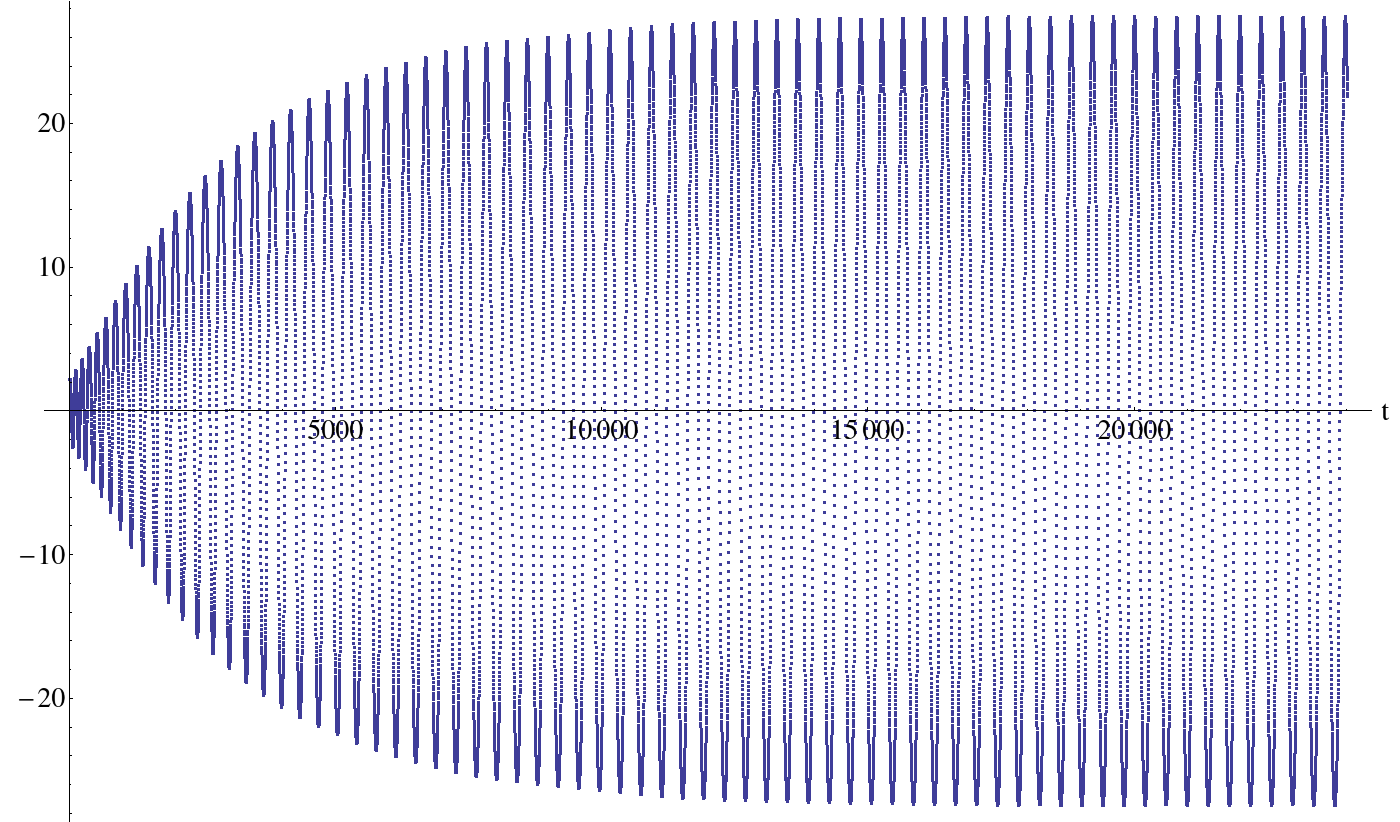
\includegraphics[scale=0.1]{Pictures/model-organisms/model-leg/Modelleg-0g-100s-friction1010-force0-7-damping0-xyz-signal.png}
};
\node[align=left] at (2.8,0.16){\scriptsize z};
\node[align=left] at (7.9,-1.5){\scriptsize t};


\draw [decoration={markings,mark=at position 1 with
    {\arrow[scale=3,>=stealth]{>}}},postaction={decorate}] (1.7,-1.3) -- (2.7,-1.3);


\draw [decoration={markings,mark=at position 1 with
    {\arrow[scale=3,>=stealth]{>}}},postaction={decorate}] (7,-2.8) -- (10.7,-4.8) node [pos=0.35, below] {applied as$~~~~~~~~~$} node [pos=0.6, below] {Torque $T~~~~~~~~~$};


%###############################################
% joint state
%###############################################

\shade[top color=white, bottom color=black!40] (8.4,-3) rectangle (13.6,-1.26);
\shade[bottom color=white, top color=black!40] (8.4,-1.26) rectangle (13.6,0.7);
\node[inner sep=0pt] (external-signal) at (11,-1.05)
{
\includegraphics[scale=0.11]{Pictures/model-organisms/model-leg/Modelleg-0g-100s-friction1010-force0-7-damping0-xyz-joint.png}
};
\node(joint-state) at (10,1){\underline{Joint dynamics}};

\node[align=left] at (8.6, 0.2){\scriptsize $\dot x$};
\node[align=left] at (13.75,-1.5){\scriptsize $x$};

 \draw [<->,red] (8.4,-2.2) -- (13.6,-2.2);
 \draw [dashed, red,thick] (8.4,0.5) -- (8.4,-3);
 \draw[dashed,red,thick] (13.6,0.5) -- (13.6,-3);
 

%###############################################
% joint
%###############################################
\begin{scope}[shift=(0:10), rotate=0] % x offset
\begin{scope}[shift=(-90:6), rotate=-90] % y offset
	\begin{scope}[shift=(90:0), rotate=90,local bounding box=joint-scope]
	
    \link(\thetaone:\Lone);
    \begin{scope}[shift=(\thetaone:\Lone), rotate=\thetaone]
        \link(\thetatwo:\Ltwo);
        \joint
        % joint damper
        \angdamper{-180}{250}{Angular damper}
        % joint limits
        \limitann{\limitzero}{\limitone}{Joint Limits}
    \end{scope}
    
    \end{scope}
\end{scope}
\end{scope}


 
\begin{pgfonlayer}{background}
  \node(controller-state-box)[bigbox] [fit = (controller-state) (internal-signal-box)] {};
  \node(joint-dynamics-box)[bigbox] [fit=(joint-scope) (external-signal) (joint-state)]{};
\end{pgfonlayer}

\end{tikzpicture}


\caption[The directly limited chaotic controller and joint complex]{The directly limited chaotic controller and its interaction with the joint. The limiters defined through the environment and the joint properties constrain both the movement of the joint and the phase space of the chaotic controller. Through the constraint within the phase space, the controller can not exhibit its full dynamics any more and it stabilizes in certain periodic oscillations defined by the parameters.}
\label{figure:direct-limit-controller-joint-complex}
\end{figure}

For the second experiment, a locally influenced chaotic controller was used. %
%
The chaotic controller output is ruled by three differential equations defined for \(\frac{dx}{dt},\frac{dy}{dt} \text{ and } \frac{dz}{dt}\) which influence the current state of the system stored in \(x(t),y(t) \text{ and } z(t)\). %
%
In this experiment, the controller is limited using the position sensor and the velocity sensor of the joint degree of freedom the controller controls. %
%
As outlined below, the following limiter configuration was found experimentally: Before every integration step, the controller state \(x(t)\) is replaced by the position sensor output and the controller state \(y(t)\) is replaced by the velocity sensor output. %
%
The limiter system imposes limiters on two of the three dimensions in the situation where the body part motion itself is limited due to a collision with ground or other body parts. %
%
In case of a collision, the joint velocity of the DoF drops and the position comes to a halt. %
%
This limits the chaotic controller in two different ways, and it is in question what trajectories will be generated by the system. %
%
The limiter setup used in a model organism is then used to observe the influence of gravity, friction and damping on the chaotic system. %
%
If it is found to be experimentally successful and the trajectories exhibit periodic or quasi-periodic movement or interleaving periodic-chaotic sequences different from the usual intrinsic chaotic motion of the underlying chaotic system, it will be used in evolutionary settings to evolve creatures controlled with it.

\subsubsection{Limiting the Model Leg in the Simulator}
\label{subsubsec:limiting-the-model-leg}

First, the different limiter configurations with z(t) as a torque output were tested on the model leg. %
%
The model leg is positioned slightly above the ground, so that if starting with zero gravity, the body part floats and moves freely without touching the ground. %
%
In the tables below, the friction values are therefore omitted when there is zero gravity. %
%
The initial conditions for the chaotic controller controlling are set to \((-1.5,0,2)\) in all experiments unless stated otherwise. %
%
When stated that the sensor X limits the x dimension, this means that the value x(t) of the dimension x is replaced with the X sensor value in every cycle. %
%
The following plots always show the phase space of the chaotic controller on the left side and the sensor space of the controlled joint DoF on the right side.

In the next plot, the dimension x is limited with the position sensor, while leaving the dimension y without limitation.

\begin{figure}[H]
	\centering
		\begin{minipage}{1.3\textwidth}
	\hspace*{-5em}
	\begin{tikzpicture}

% classes
\pgfdeclarelayer{background}
\pgfdeclarelayer{foreground}
\pgfsetlayers{background,main,foreground}
\tikzstyle{bigbox} = [draw=black!80, thick, fill=black!5, rounded corners, rectangle]
\tikzstyle{box} = [minimum size=0.6cm, rounded corners,rectangle, fill=black!50]

\node[align=left] at (0,0){\underline{Controller State Space}};
\node[inner sep=0pt] (controller-state-space) at (0,-3)
{
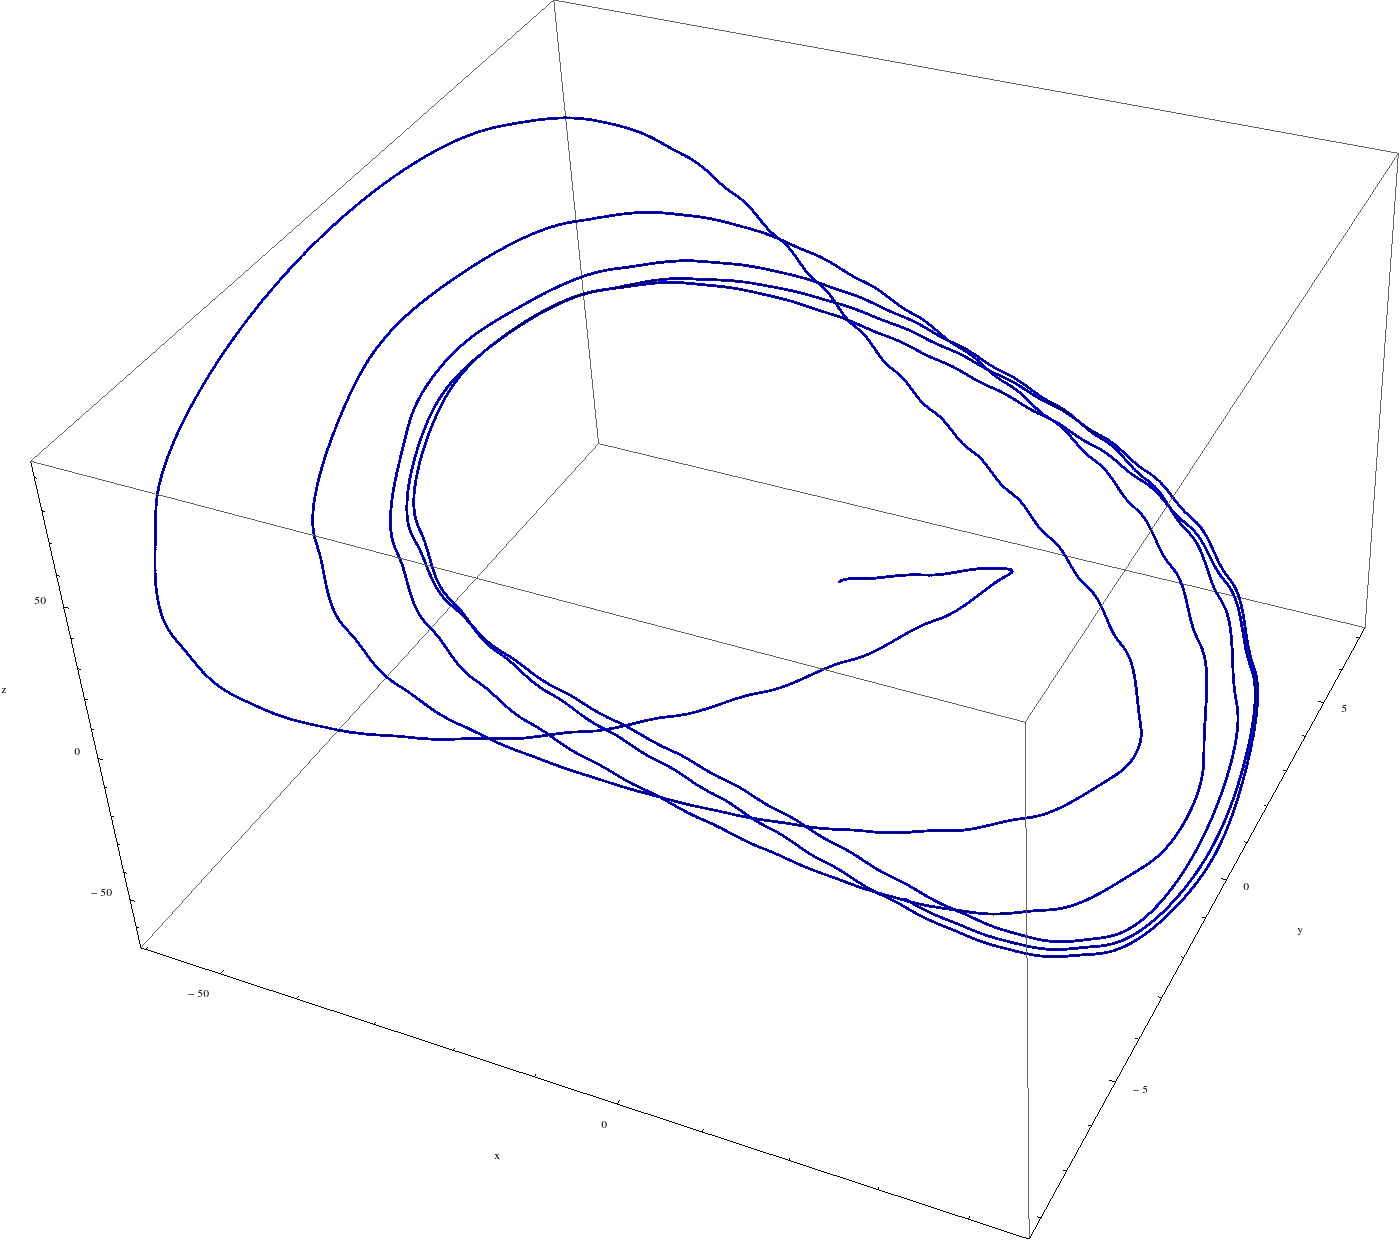
\includegraphics[width=0.45\textwidth]{model-organisms/model-leg/Modelleg-px(y)z-0g-force-0-00007-damping-0.png}
};

\node[align=left] at (9,0){\underline{Joint Dynamics}};
\node[inner sep=0pt] (joint-dynamics) at (9,-3)
{
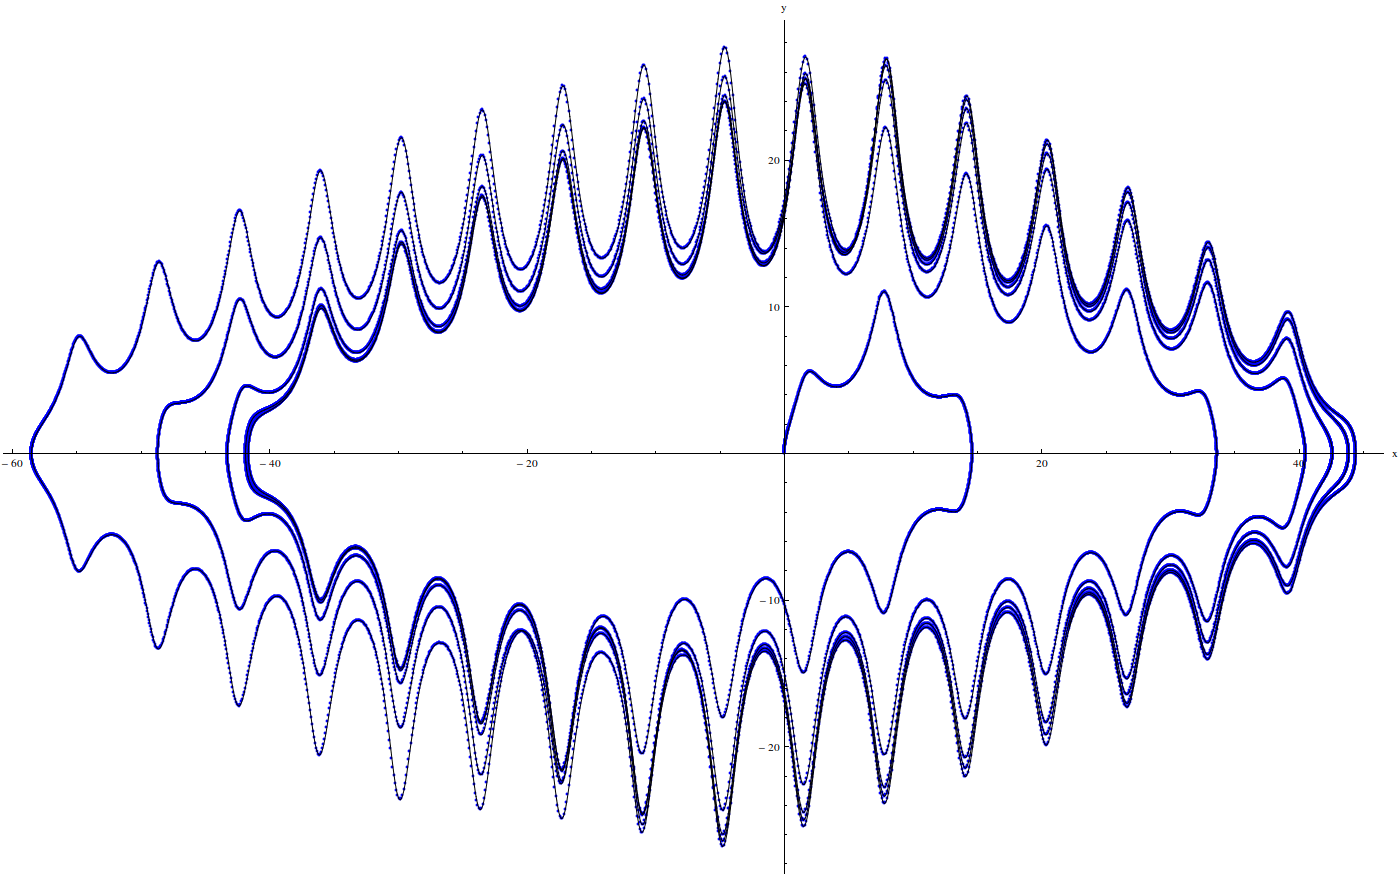
\includegraphics[width=0.45\textwidth]{model-organisms/model-leg/Modelleg-px(y)z-0g-force-0-00007-damping-0-joint.png}
};
	\end{tikzpicture}
	\end{minipage}
	\caption[Joint position \(\rightarrow\) x(t) limited chaotic controller controlling model leg.]{A strange quasi-periodic limit cycle can be observed in the chaotic controller phase space and the sensor space. The model body part oscillates strangely.}
	\begin{tabular}{l|ll}
	\hline 
	Gravity: 0g  & Sensors: & Joint position \(\rightarrow\) x(t)\\
	 Output: z(t) \(\rightarrow\) Joint torque & & - \\
	  Torque scaling curve: \(0.7~(mass_1~\cdot~mass_2)\) & & - \\
	  \hline
	\end{tabular}
	\label{figure:limited-model-leg1}
\end{figure}

When switching the limited dimension from x to y, the following strange trajectory can be observed in the sensor space.

\begin{figure}[H]
	\centering
	\begin{minipage}{1.3\textwidth}
	\hspace*{-5em}
	\begin{tikzpicture}

% classes
\pgfdeclarelayer{background}
\pgfdeclarelayer{foreground}
\pgfsetlayers{background,main,foreground}
\tikzstyle{bigbox} = [draw=black!80, thick, fill=black!5, rounded corners, rectangle]
\tikzstyle{box} = [minimum size=0.6cm, rounded corners,rectangle, fill=black!50]

\node[align=left] at (0,0){\underline{Controller State Space}};
\node[inner sep=0pt] (controller-state-space) at (0,-3)
{
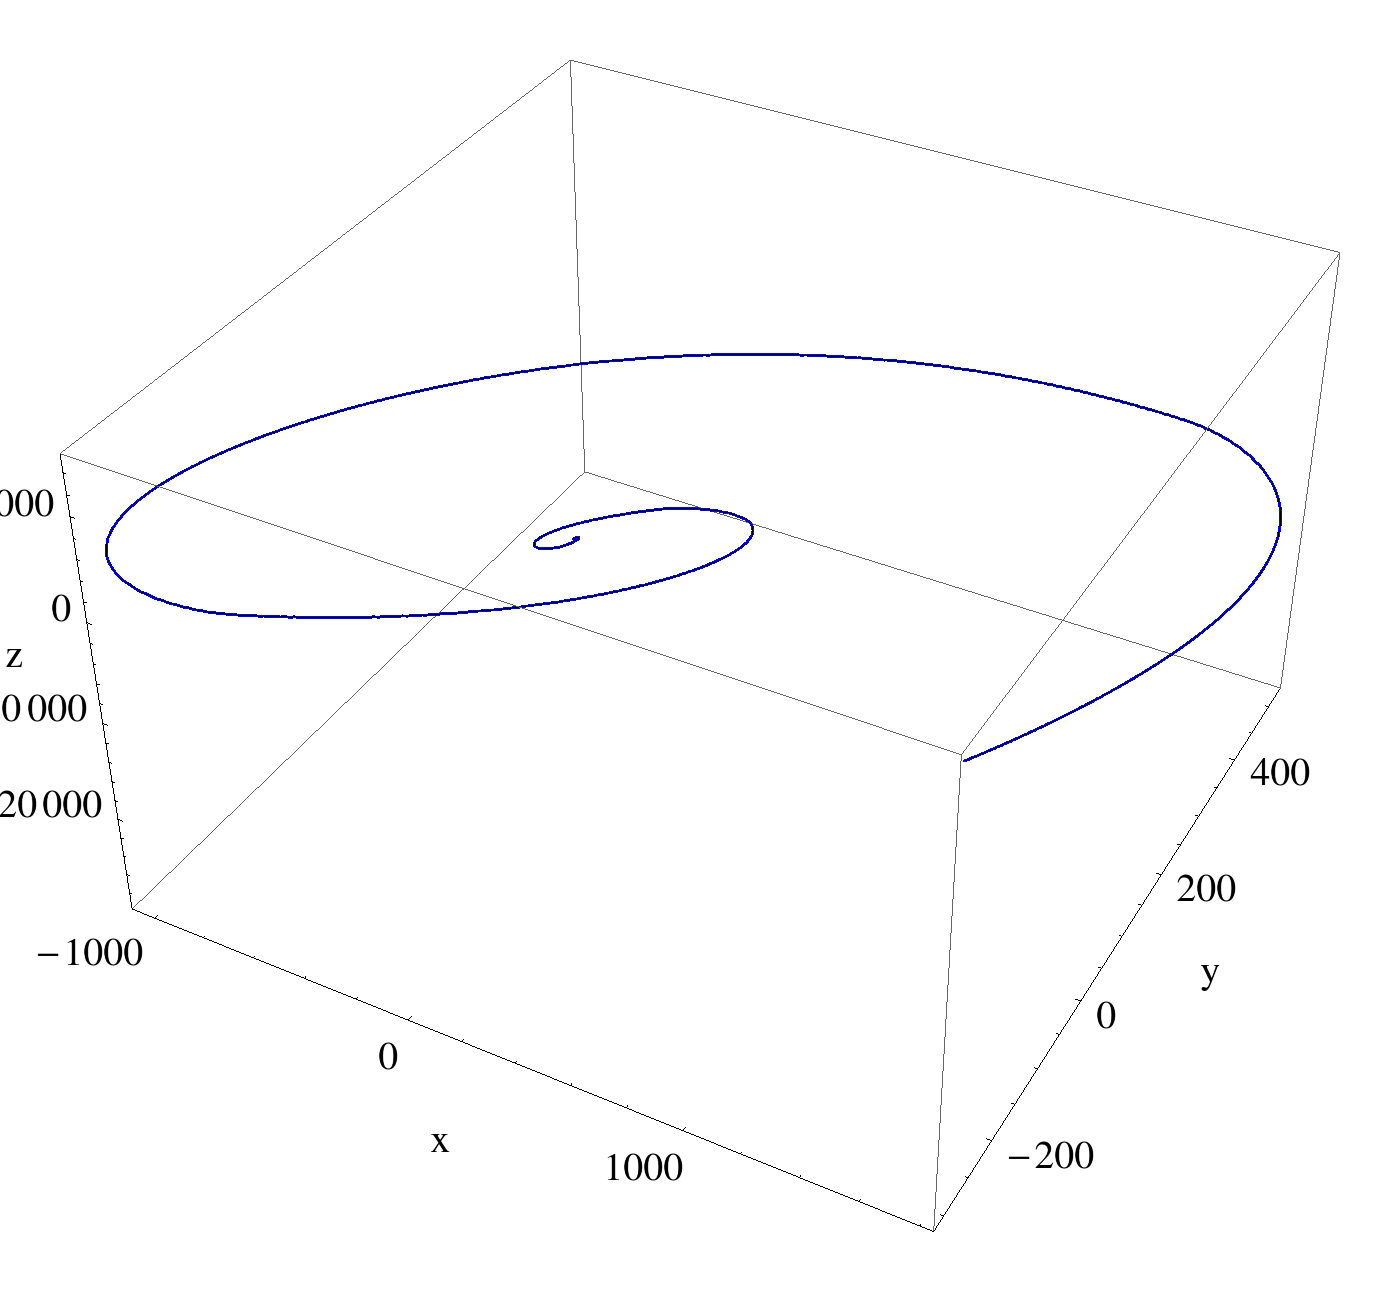
\includegraphics[width=0.45\textwidth]{model-organisms/model-leg/Modelleg-(x)pyz-0g-force-0-00007-damping-0.png}
};

\node[align=left] at (9,0){\underline{Joint Dynamics}};
\node[inner sep=0pt] (joint-dynamics) at (9,-3)
{
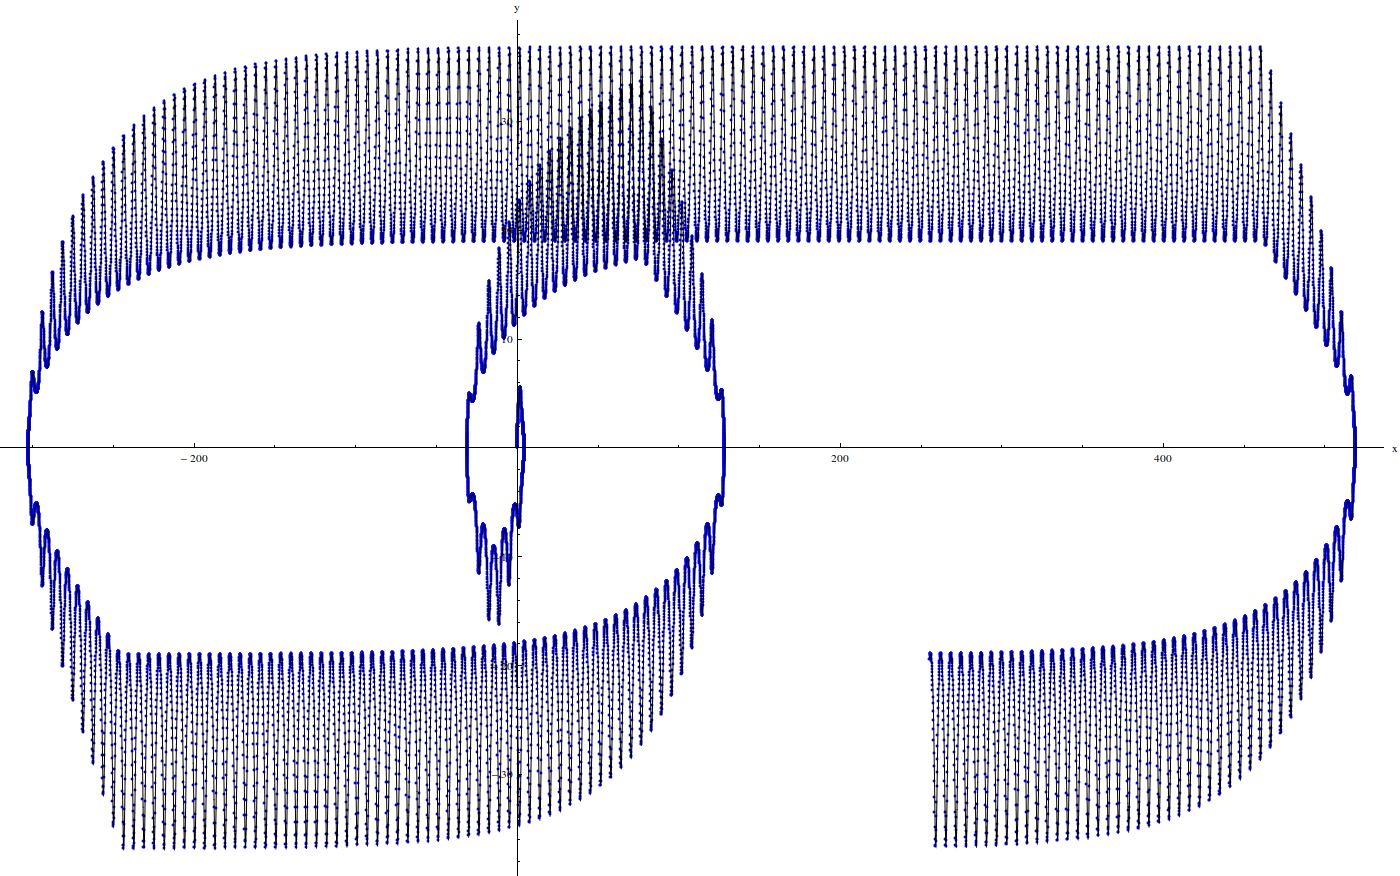
\includegraphics[width=0.45\textwidth]{model-organisms/model-leg/Modelleg-(x)pyz-0g-force-0-00007-damping-0-joint.png}
};
	\end{tikzpicture}
	\end{minipage}
	\caption[Joint position \(\rightarrow\) y(t) limited chaotic controller controlling model leg]{In the chaotic controller, one can observe an outward spiral, which indicates that the joint position limiting the y dimension turns the original attractor into a repeller.}
	\begin{tabular}{l|ll}
	\hline 
	Gravity: 0g  & Sensors: & Joint position \(\rightarrow\) y(t)\\
	 Output: z(t) \(\rightarrow\) Joint torque & & - \\
	  Torque scaling curve: \(0.7~(mass_1~\cdot~mass_2)\) & & - \\
	  \hline
	\end{tabular}

	\label{figure:limited-model-leg2}
\end{figure}

If the same dimensions are limited by the velocity sensor instead of the position sensor, a behavior as shown in figure \ref{figure:limited-model-leg3} can be observed.

\begin{figure}[H]
	\centering
	\begin{minipage}{1.3\textwidth}
	\hspace*{-5em}
	\begin{tikzpicture}

% classes
\pgfdeclarelayer{background}
\pgfdeclarelayer{foreground}
\pgfsetlayers{background,main,foreground}
\tikzstyle{bigbox} = [draw=black!80, thick, fill=black!5, rounded corners, rectangle]
\tikzstyle{box} = [minimum size=0.6cm, rounded corners,rectangle, fill=black!50]

\node[align=left] at (0,0){\underline{Controller State Space}};
\node[inner sep=0pt] (controller-state-space) at (0,-3)
{
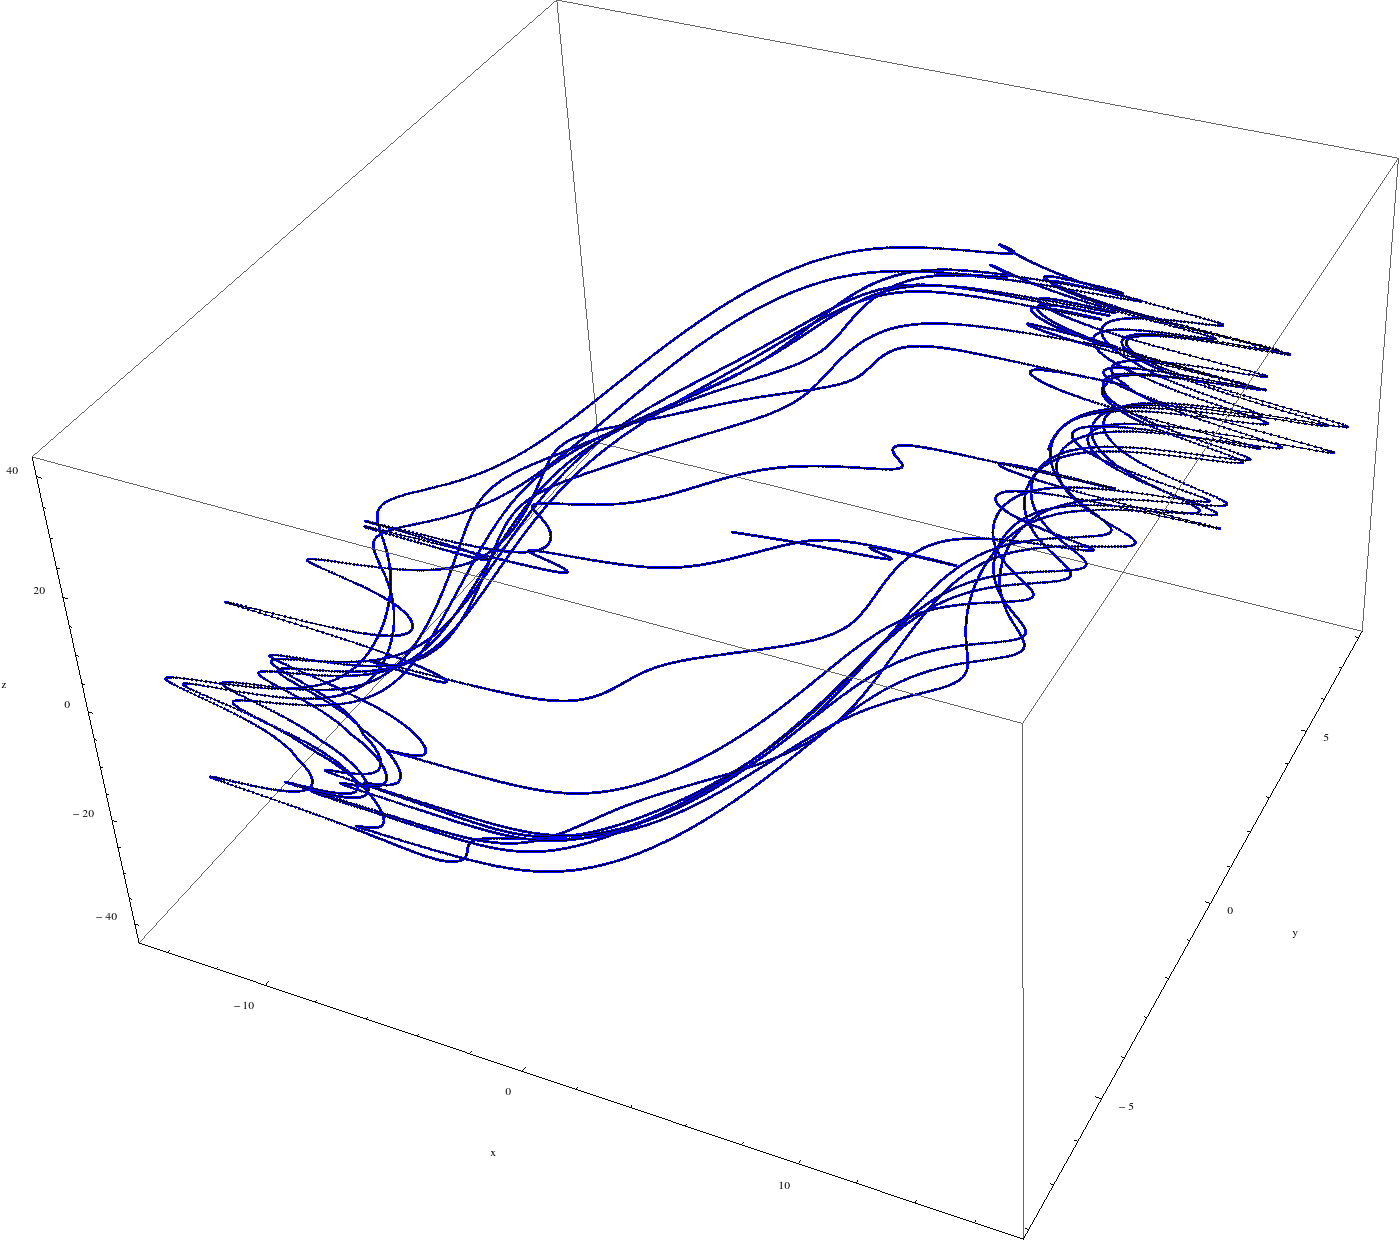
\includegraphics[width=0.45\textwidth]{model-organisms/model-leg/Modelleg-vx(y)z-0g-force-0-00007-damping-0.png}
};

\node[align=left] at (9,0){\underline{Joint Dynamics}};
\node[inner sep=0pt] (joint-dynamics) at (9,-3)
{
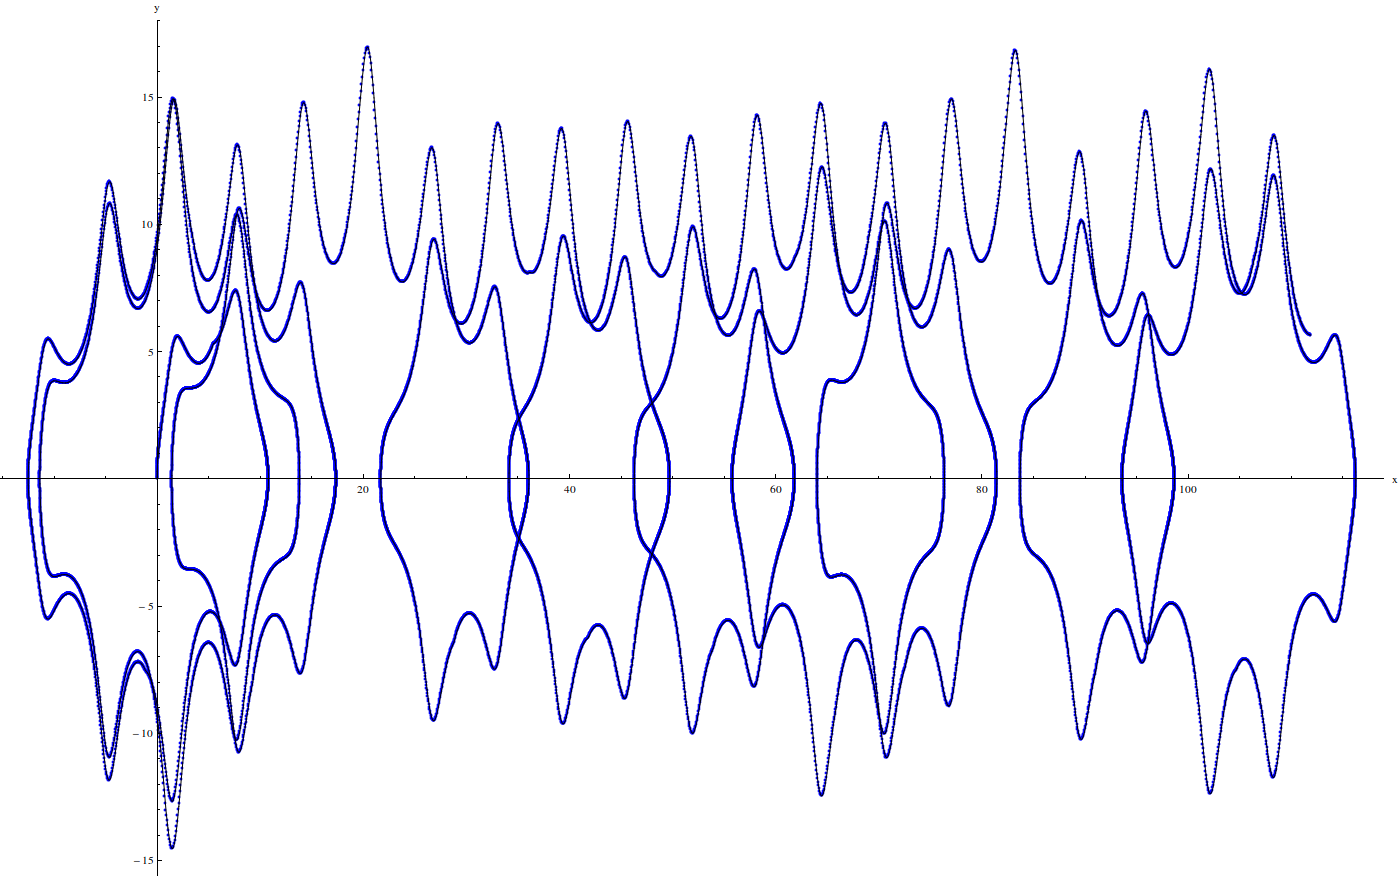
\includegraphics[width=0.45\textwidth]{model-organisms/model-leg/Modelleg-vx(y)z-0g-force-0-00007-damping-0-joint.png}
};
	\end{tikzpicture}
	\end{minipage}
	\caption[Joint Velocity \(\rightarrow\) x(t) limited chaotic controller controlling model leg]{A strange quasi-periodic limit cycle can be observed in the controller phase space, but not in the sensor space. The velocity of the joint moves in a strange oscillation around zero, resulting in a net increase of the position.}
	\begin{tabular}{l|ll}
	\hline 
	Gravity: 0g  & Sensors: & Joint Velocity \(\rightarrow\) x(t)\\
	 Output: z(t) \(\rightarrow\) Joint torque & & - \\
	  Torque scaling curve: \(0.7~(mass_1~\cdot~mass_2)\) & & - \\
	  \hline
	\end{tabular}
	\label{figure:limited-model-leg3}
\end{figure}

If the joint velocity limits y(t) instead of x(t), the trajectory shows convergence to a limit cycle.

\begin{figure}[H]
	\centering
	\begin{minipage}{1.3\textwidth}
	\hspace*{-5em}
	\begin{tikzpicture}

% classes
\pgfdeclarelayer{background}
\pgfdeclarelayer{foreground}
\pgfsetlayers{background,main,foreground}
\tikzstyle{bigbox} = [draw=black!80, thick, fill=black!5, rounded corners, rectangle]
\tikzstyle{box} = [minimum size=0.6cm, rounded corners,rectangle, fill=black!50]

\node[align=left] at (0,0){\underline{Controller State Space}};
\node[inner sep=0pt] (controller-state-space) at (0,-3)
{
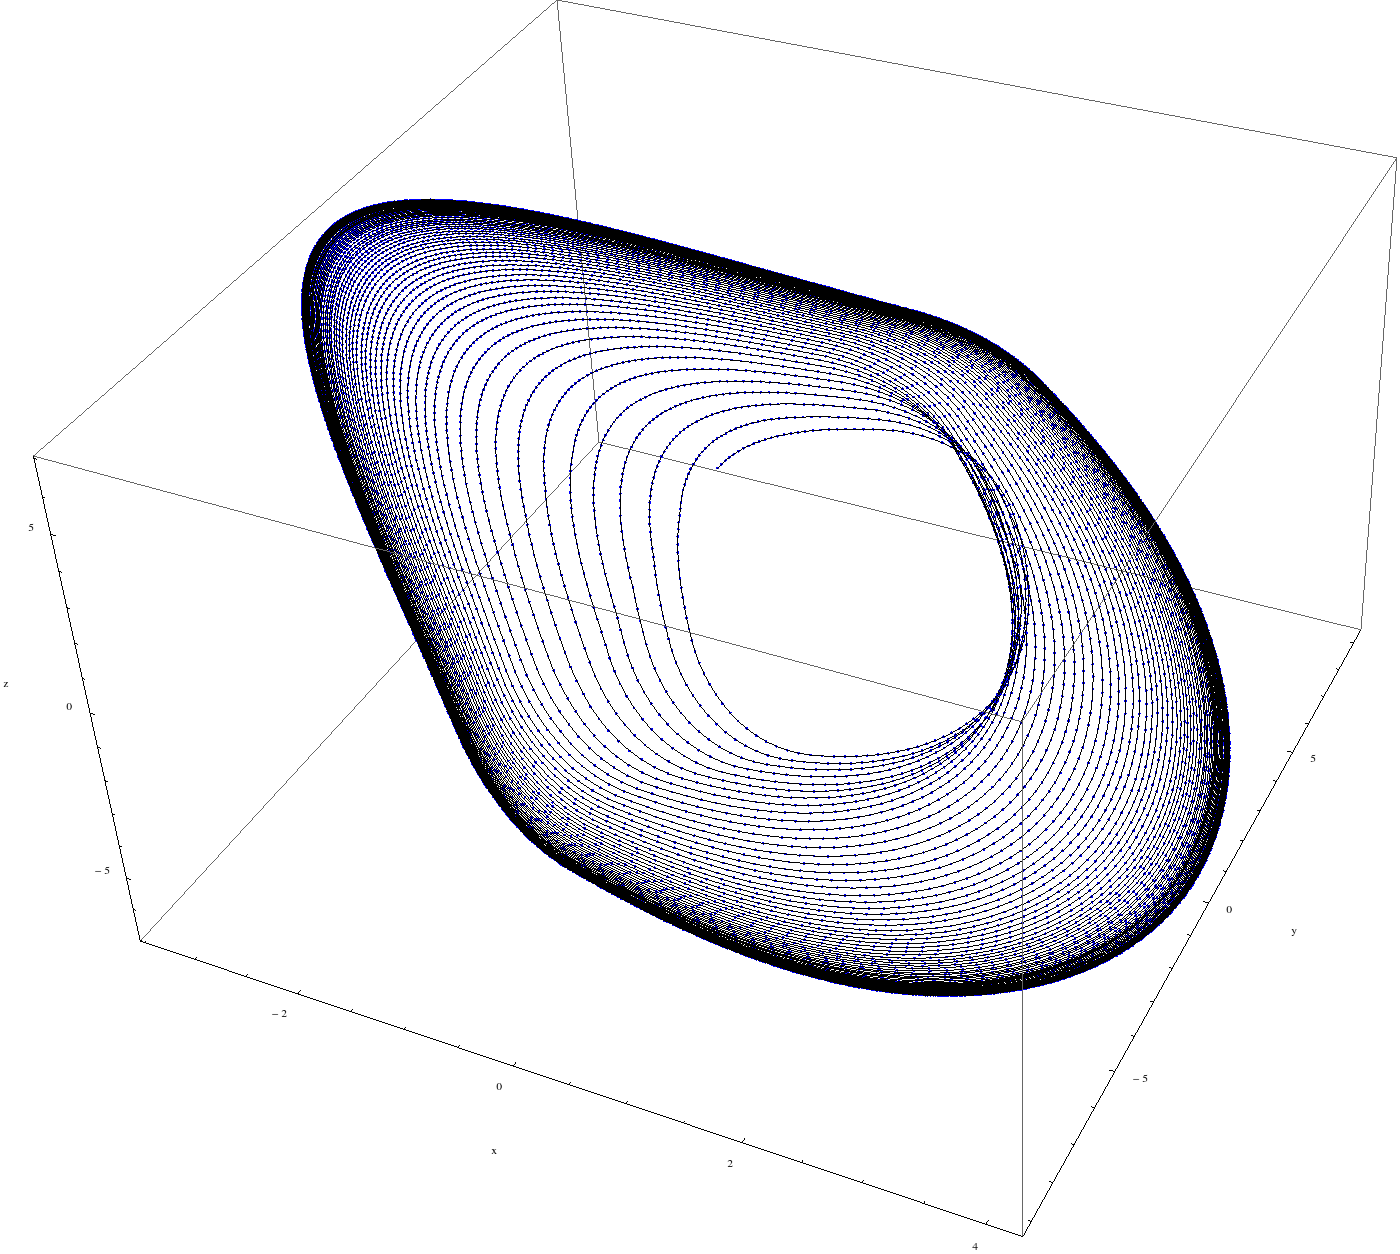
\includegraphics[width=0.45\textwidth]{model-organisms/model-leg/Modelleg-(x)vyz-0g-force-0-00007-damping-0.png}
};

\node[align=left] at (9,0){\underline{Joint Dynamics}};
\node[inner sep=0pt] (joint-dynamics) at (9,-3)
{
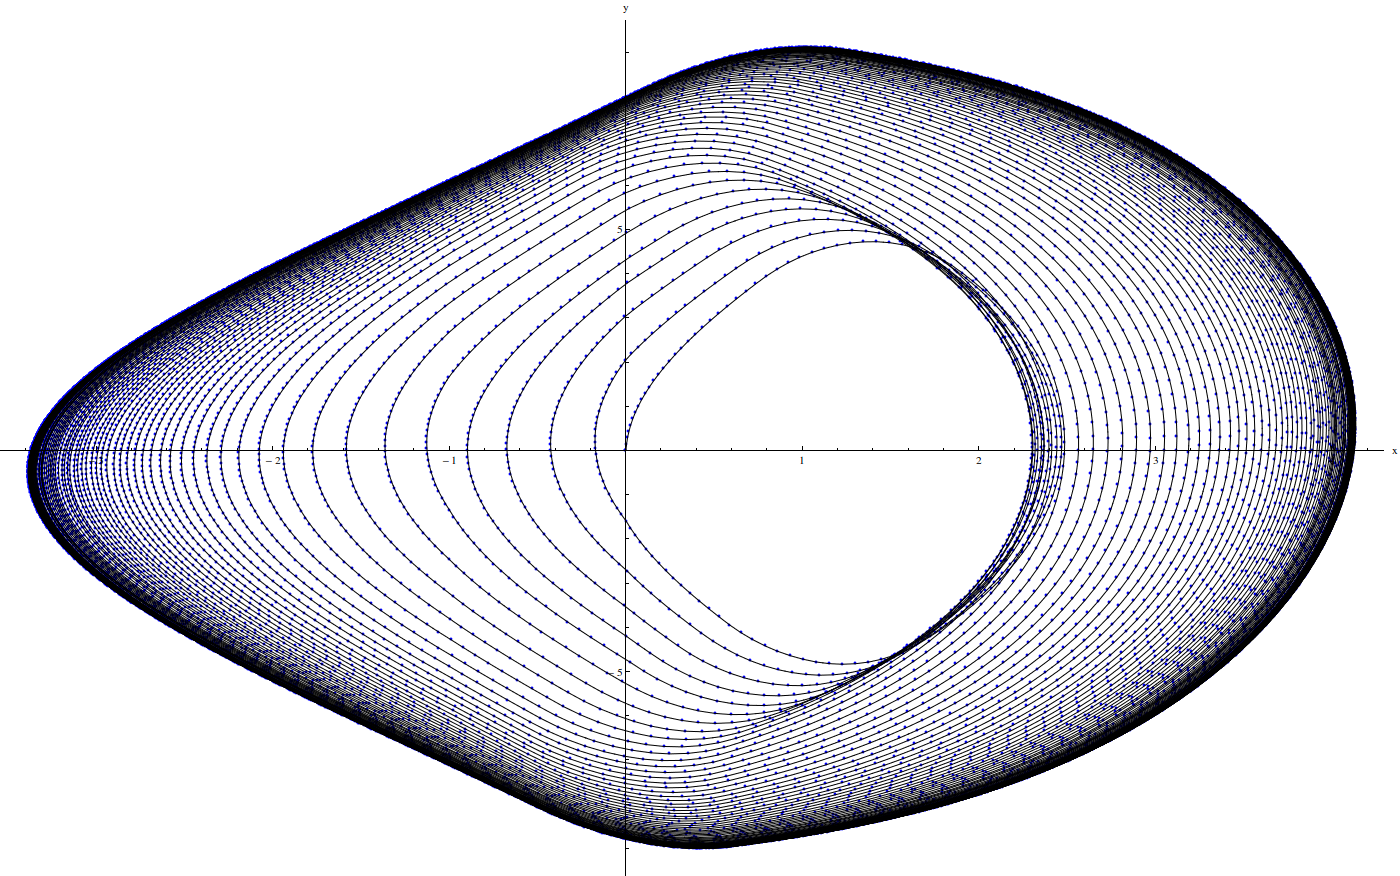
\includegraphics[width=0.45\textwidth]{model-organisms/model-leg/Modelleg-(x)vyz-0g-force-0-00007-damping-0-joint.png}
};
	\end{tikzpicture}
	\end{minipage}
	\caption[Joint Velocity \(\rightarrow\) y(t) limited chaotic controller controlling model leg]{The trajectory performs symmetrical outward spiral which approaches a limit cycle of periodicity 1 at the outer bounds. This behavior can be explained by the fact that in the Chua equations, a simple negative feedback cycle is constructed. If the velocity increases into the positive direction, z(t) gets driven into the negative direction, therefore a torque pointing into the opposite direction is applied. Additionally a descent down into the plane of the periodic orbit can be observed.}
	\begin{tabular}{l|ll}
	\hline 
	Gravity: 0g  & Sensors: & Joint Velocity \(\rightarrow\) y(t)\\
	 Output: z(t) \(\rightarrow\) Joint torque &  & - \\
	  Torque scaling curve: \(0.7~(mass_1~\cdot~mass_2)\) & & - \\
	  \hline
	\end{tabular}

	\label{figure:limited-model-leg4}
\end{figure}

If two successful limiters get combined, namely the Joint position \(\rightarrow\) x(t) resulting in a strange limit cycle and Joint Velocity \(\rightarrow\) y(t) resulting in a smoother limit cycle, the resulting limit cycle looks as follows.

\begin{figure}[H]
	\centering
	\begin{minipage}{1.3\textwidth}
	\hspace*{-5em}
	\begin{tikzpicture}

% classes
\pgfdeclarelayer{background}
\pgfdeclarelayer{foreground}
\pgfsetlayers{background,main,foreground}
\tikzstyle{bigbox} = [draw=black!80, thick, fill=black!5, rounded corners, rectangle]
\tikzstyle{box} = [minimum size=0.6cm, rounded corners,rectangle, fill=black!50]

\node[align=left] at (0,0){\underline{Controller State Space}};
\node[inner sep=0pt] (controller-state-space) at (0,-3)
{
\includegraphics[width=0.45\textwidth]{model-organisms/model-leg/Modelleg-0g-100s-friction1010-force0-7-damping0-xyz.png}
};

\node[align=left] at (9,0){\underline{Joint Dynamics}};
\node[inner sep=0pt] (joint-dynamics) at (9,-3)
{
\includegraphics[width=0.45\textwidth]{model-organisms/model-leg/Modelleg-0g-100s-friction1010-force0-7-damping0-xyz-joint.png}
};
	\end{tikzpicture}
	\end{minipage}
	\caption[Joint position \(\rightarrow\) x(t) and Joint Velocity \(\rightarrow\) y(t) limited chaotic controller controlling model leg]{The shape of the limit cycle gets distorted.}
	\begin{tabular}{l|ll}
	\hline 
	Gravity: 0g  & Sensors: & Joint position \(\rightarrow\) x(t),\\
	 Output: z(t) \(\rightarrow\) Joint torque &  & Joint Velocity \(\rightarrow\) y(t) \\
	  Torque scaling curve: \(0.7~(mass_1~\cdot~mass_2)\) & & - \\
	  \hline
	\end{tabular}

	\label{figure:limited-model-leg5}
\end{figure}

However the combination of non-stabilizing limiters does not stabilize any unstable periodic orbit.

\begin{figure}[H]
	\centering
	\begin{minipage}{1.3\textwidth}
	\hspace*{-5em}
	\begin{tikzpicture}

% classes
\pgfdeclarelayer{background}
\pgfdeclarelayer{foreground}
\pgfsetlayers{background,main,foreground}
\tikzstyle{bigbox} = [draw=black!80, thick, fill=black!5, rounded corners, rectangle]
\tikzstyle{box} = [minimum size=0.6cm, rounded corners,rectangle, fill=black!50]

\node[align=left] at (0,0){\underline{Controller State Space}};
\node[inner sep=0pt] (controller-state-space) at (0,-3)
{
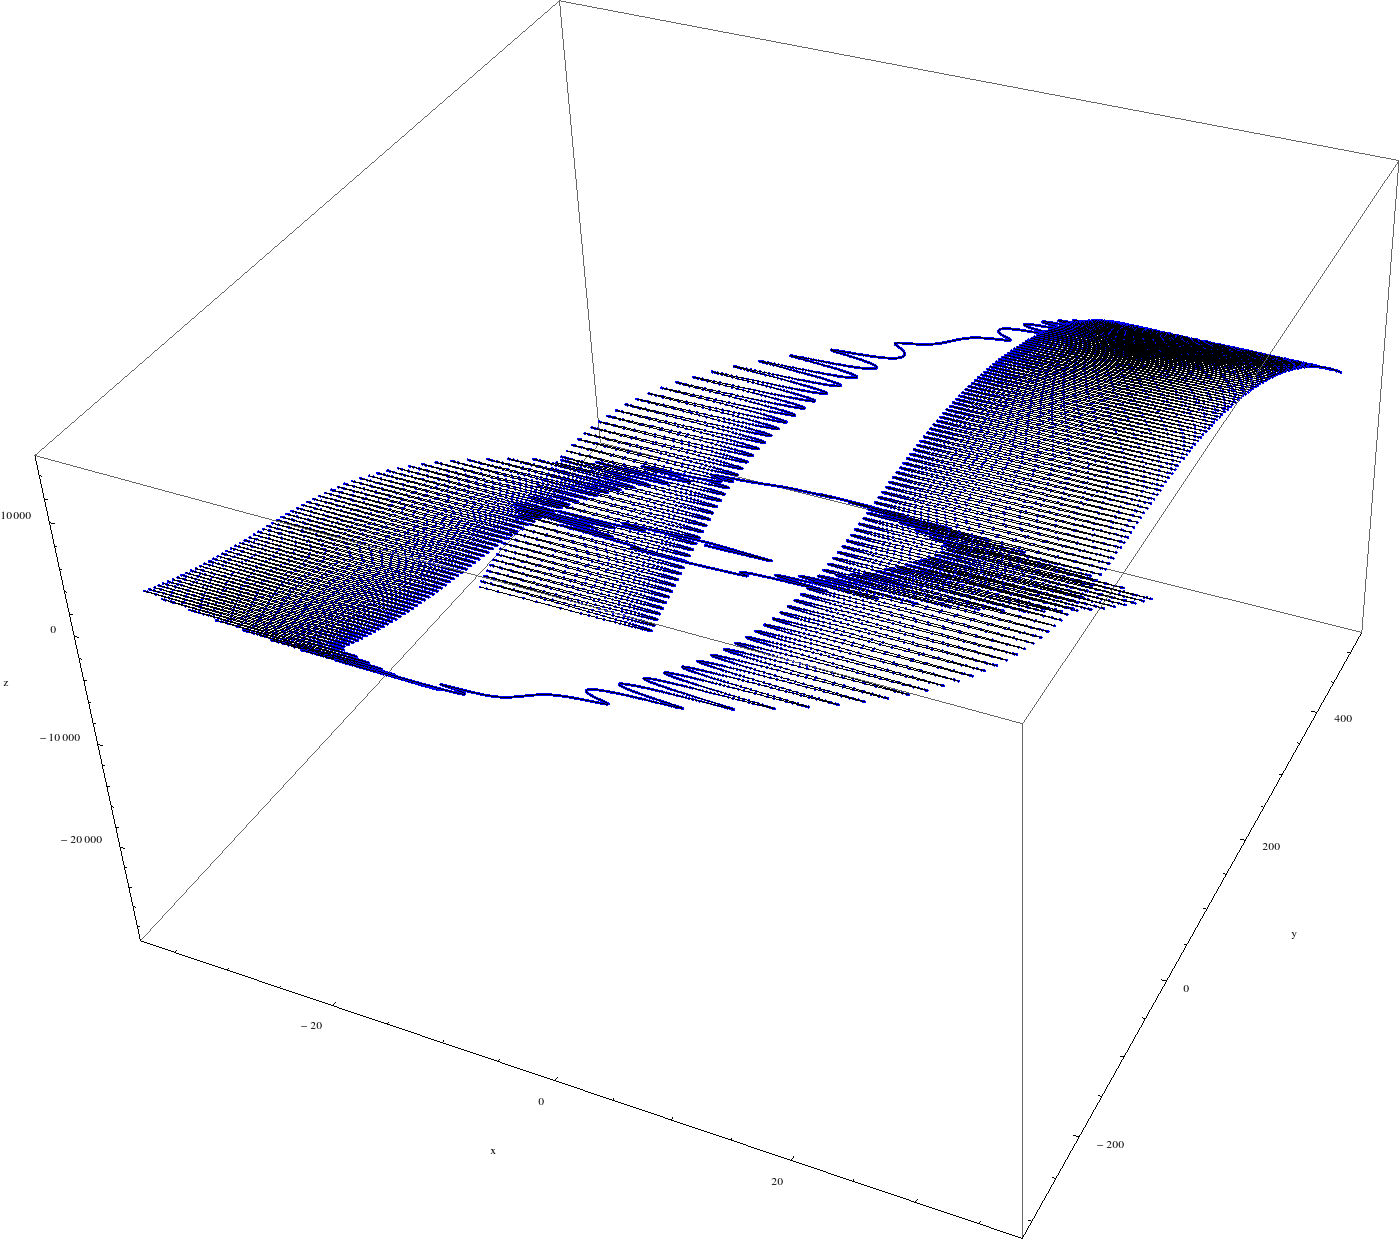
\includegraphics[width=0.45\textwidth]{model-organisms/model-leg/Modelleg-vxpyz-0g-force-0-00007-damping-0.png}
};

\node[align=left] at (9,0){\underline{Joint Dynamics}};
\node[inner sep=0pt] (joint-dynamics) at (9,-3)
{
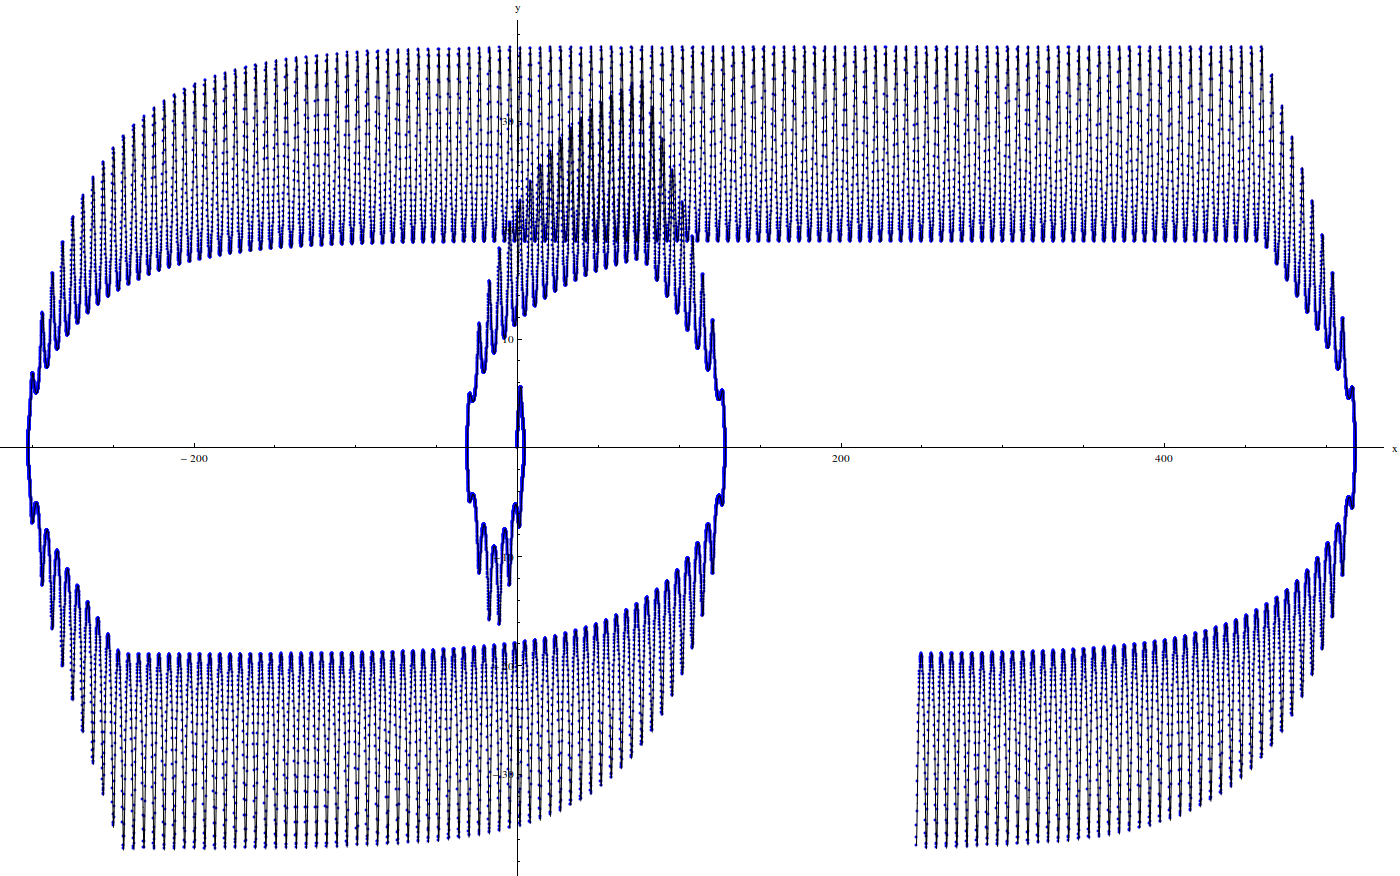
\includegraphics[width=0.45\textwidth]{model-organisms/model-leg/Modelleg-vxpyz-0g-force-0-00007-damping-0-joint.png}
};
	\end{tikzpicture}
	\end{minipage}
	\caption[Joint Velocity \(\rightarrow\) x(t) and Joint Position \(\rightarrow\) y(t) limited chaotic controller controlling model leg]{A strangely oscillating trajectory can be observed.}
	\begin{tabular}{l|ll}
	\hline 
	Gravity: 0g  & Sensors: & Joint Velocity \(\rightarrow\) x(t),\\
	 Output: z(t) \(\rightarrow\) Joint torque & & Joint Position \(\rightarrow\) y(t) \\
	  Torque scaling curve: \(0.7~(mass_1~\cdot~mass_2)\) & & - \\
	  \hline
	\end{tabular}

	\label{figure:limited-model-leg6}
\end{figure}

The configuration where the x dimension is limited with the position sensor and the y dimension is limited with the velocity sensor is chosen for further examination. %
%
Based on this configuration, the model leg with different joint torques, friction and damping coefficients was simulated to observe the resulting change in controller and joint dynamics. %
%
In the following plots, different influencing factors on the limit cycle are shown:

\paragraph{Interaction with Ground} The ground imposes a very hard limiter onto the creature. %
%
The movement of the creature gets instantly stopped, whereas the ground has infinite mass and therefore is not influenced by the creature. %
%
In some cases, the ground should therefore directly act as a very hard limiter onto the chaotic circuit, controlling the chaotic movement into low periods and orbits of smaller diameter as in the experiments performed in the section \ref{subsubsec:simple-limiter-mathematica}. 
%
In the first setting, the model leg is dropped onto a frictionless ground. 
\begin{figure}[H]
	\centering
	\begin{minipage}{1.3\textwidth}
	\hspace*{-5em}
	\begin{tikzpicture}

% classes
\pgfdeclarelayer{background}
\pgfdeclarelayer{foreground}
\pgfsetlayers{background,main,foreground}
\tikzstyle{bigbox} = [draw=black!80, thick, fill=black!5, rounded corners, rectangle]
\tikzstyle{box} = [minimum size=0.6cm, rounded corners,rectangle, fill=black!50]

\node[align=left] at (0,0){\underline{Controller State Space}};
\node[inner sep=0pt] (controller-state-space) at (0,-3)
{
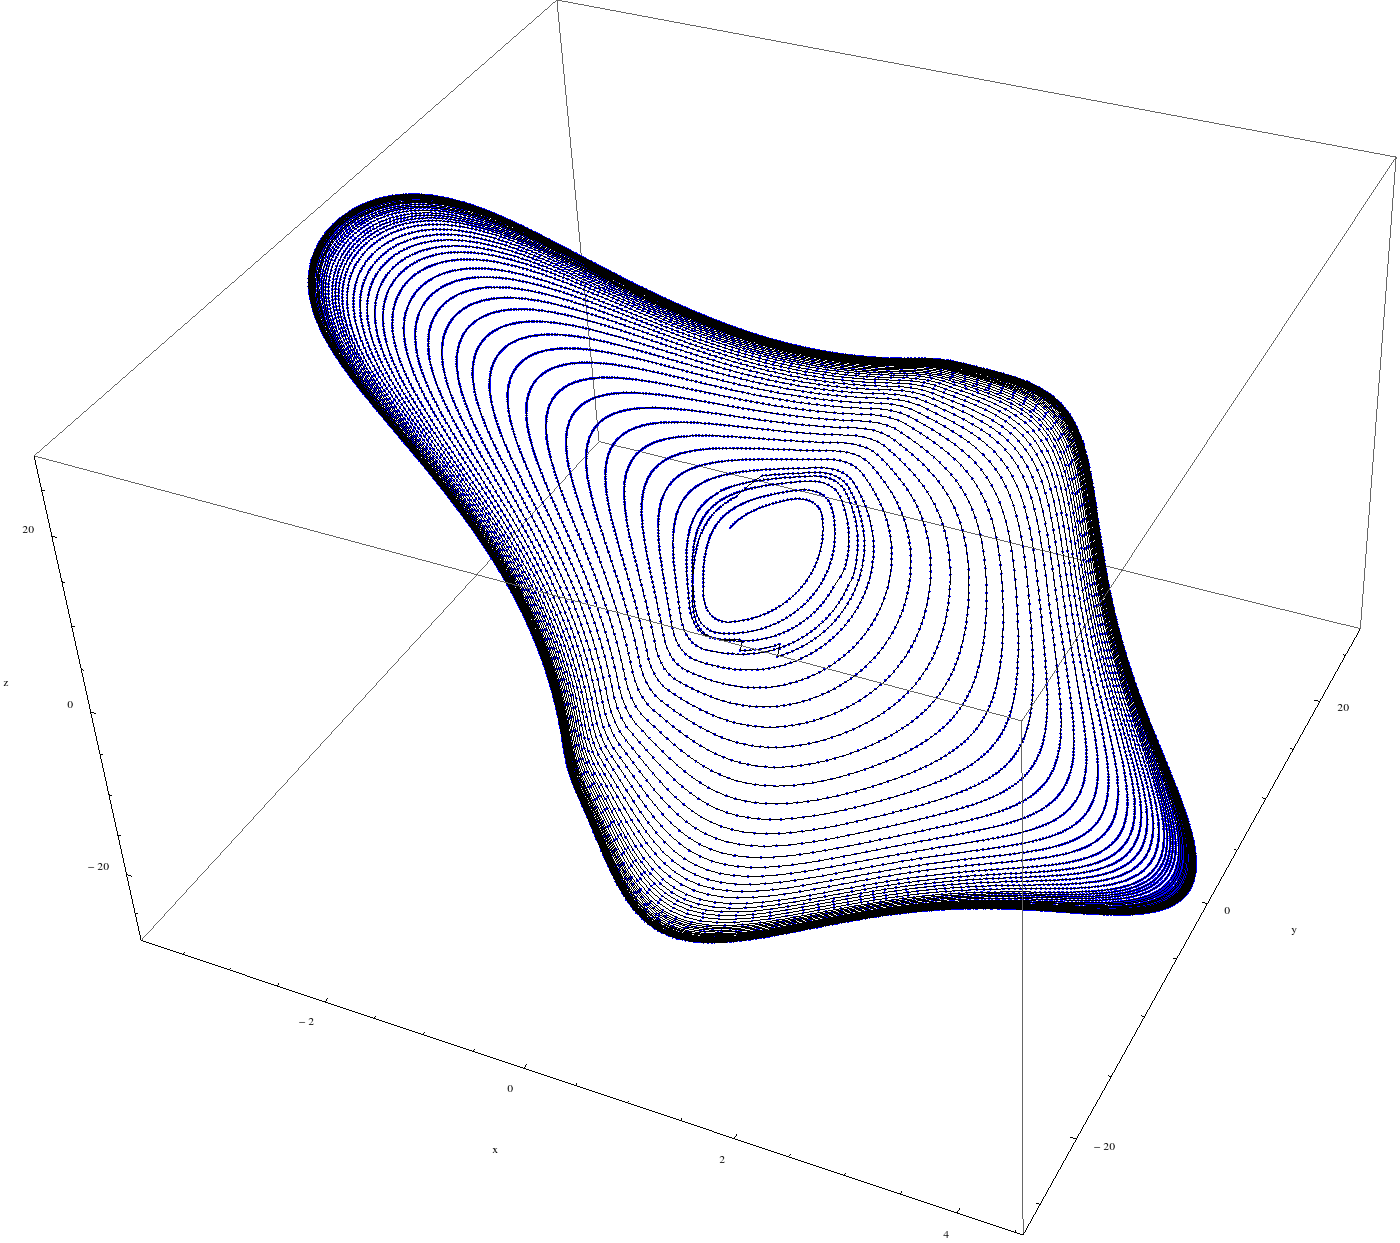
\includegraphics[width=0.45\textwidth]{model-organisms/model-leg/Modelleg-1g-100s-friction00-force0-7-damping0-xyz.png}
};

\node[align=left] at (9,0){\underline{Joint Dynamics}};
\node[inner sep=0pt] (joint-dynamics) at (9,-3)
{
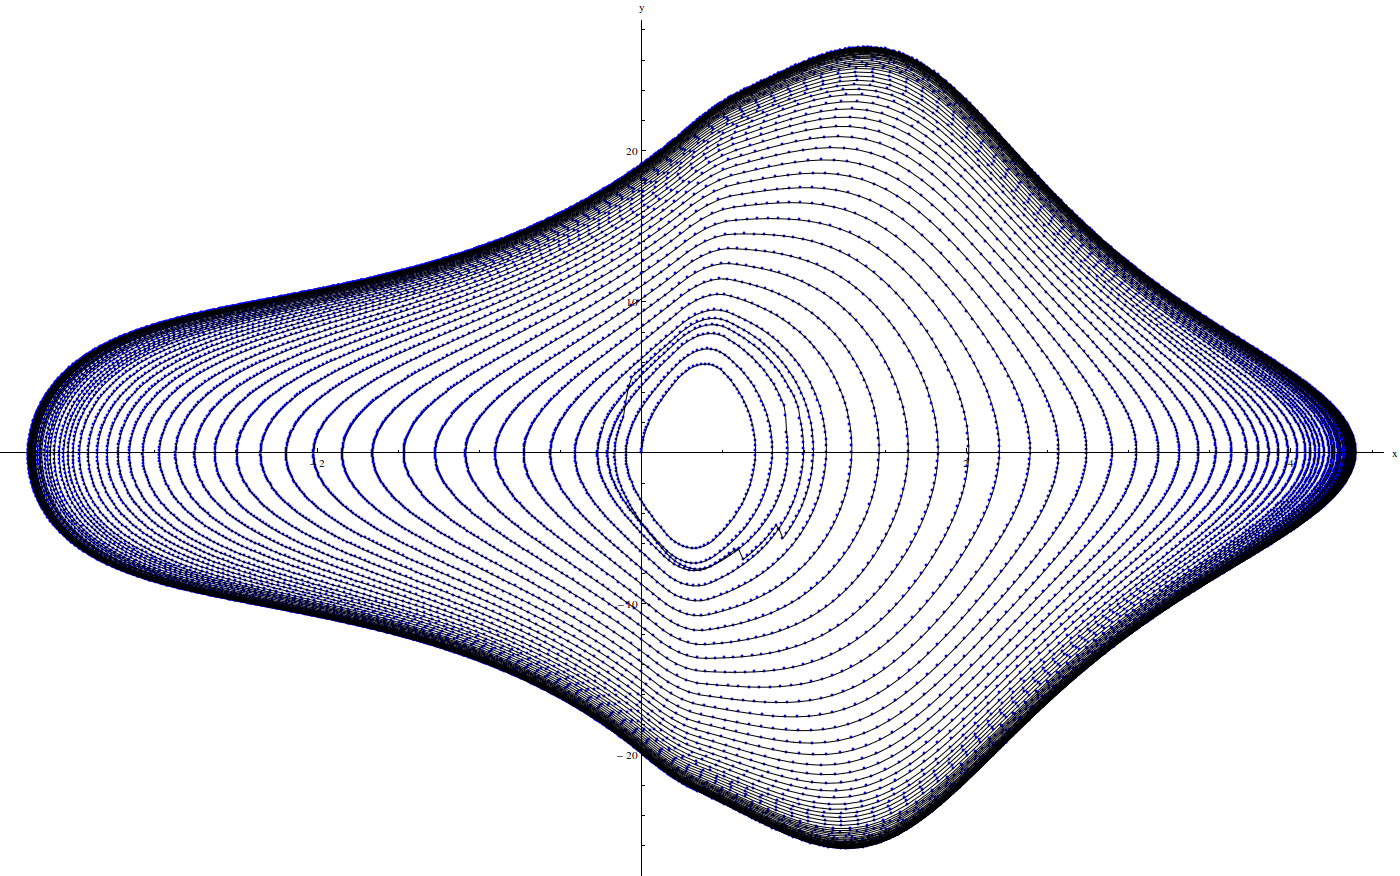
\includegraphics[width=0.45\textwidth]{model-organisms/model-leg/Modelleg-1g-100s-friction00-force0-7-damping0-xyz-joint.png}
};
	\end{tikzpicture}
	\end{minipage}
	\caption[Limited chaotic controller controlling model leg on frictionless ground.]{The interaction with ground can be observed both in the controller phase space and the sensor space. Small perturbations causing a drop of the velocity towards zero change the trajectory of the spiral. The frictionless ground limits the controller only quickly, because afterwards the model leg falls to the side, slides on the ground and converges to the original periodic orbit.}
	\begin{tabular}{l|ll}
	\hline 
	Gravity: 1g  & Sensors: & Joint position \(\rightarrow\) x(t),\\
	 Output: z(t) \(\rightarrow\) Joint torque &  & Joint Velocity \(\rightarrow\) y(t) \\
	  Torque scaling curve: \(0.7~(mass_1~\cdot~mass_2)\) & Friction: & Creature 0, Ground 0 \\
	  \hline
	\end{tabular}
	
	\label{figure:limited-damped-model-leg-collision1}
\end{figure}

Changing the friction of the ground to a non-zero value increases the limiter imposed on the controller.

\begin{figure}[H]
	\centering
	\begin{minipage}{1.3\textwidth}
	\hspace*{-5em}
	\begin{tikzpicture}

% classes
\pgfdeclarelayer{background}
\pgfdeclarelayer{foreground}
\pgfsetlayers{background,main,foreground}
\tikzstyle{bigbox} = [draw=black!80, thick, fill=black!5, rounded corners, rectangle]
\tikzstyle{box} = [minimum size=0.6cm, rounded corners,rectangle, fill=black!50]

\node[align=left] at (0,0){\underline{Controller State Space}};
\node[inner sep=0pt] (controller-state-space) at (0,-3)
{
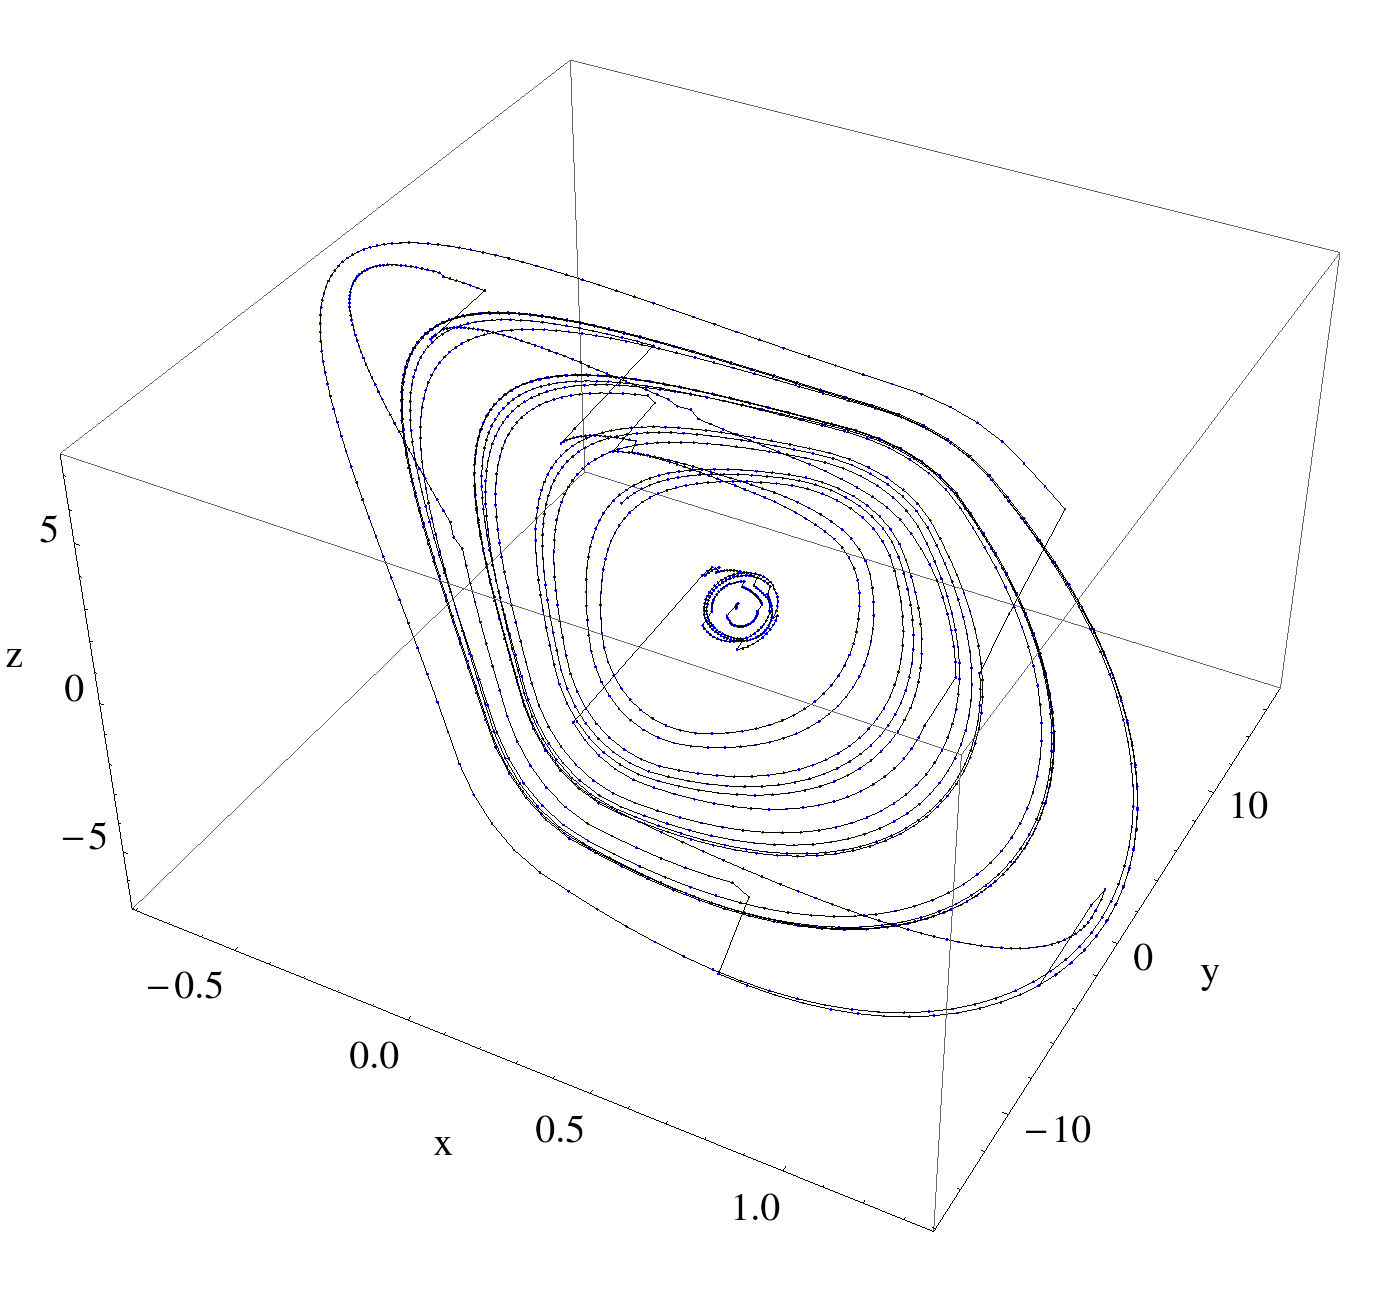
\includegraphics[width=0.45\textwidth]{model-organisms/model-leg/Modelleg-1g-100s-friction11-force2-damping0-xyz.png}
};

\node[align=left] at (9,0){\underline{Joint Dynamics}};
\node[inner sep=0pt] (joint-dynamics) at (9,-3)
{
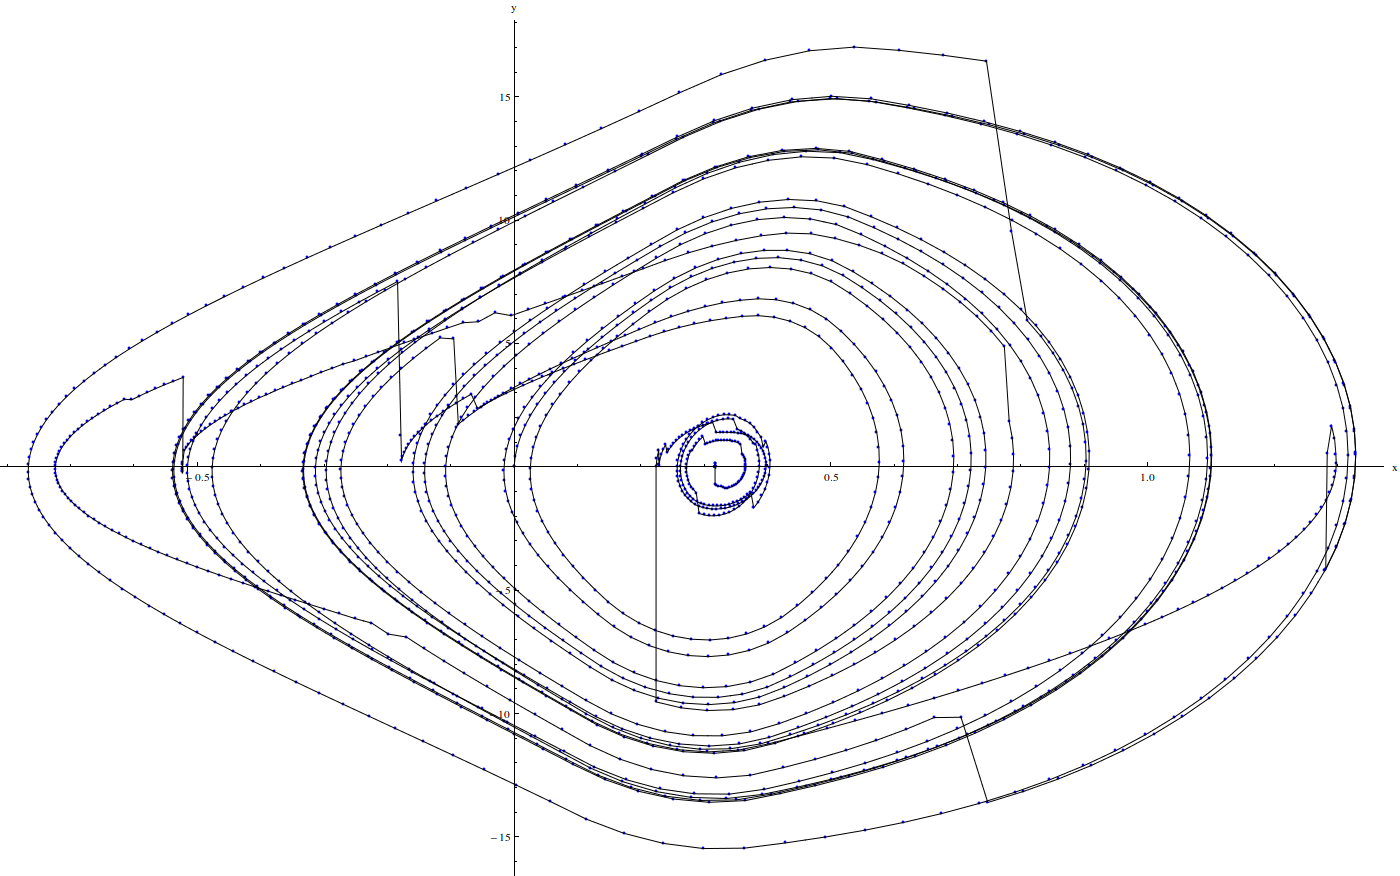
\includegraphics[width=0.45\textwidth]{model-organisms/model-leg/Modelleg-1g-100s-friction11-force2-damping0-xyz-joint.png}
};
	\end{tikzpicture}
	\end{minipage}
	\caption[Limited chaotic controller controlling model leg on ground with friction]{The ground with friction now shows a much more influential limiter. The model leg hits the ground several times while oscillating, which stabilizes several periodic orbits for one to two cycles. Finally the model leg comes to a rest as it blocks the oscillation as it falls to the ground while completely extended.}
	\begin{tabular}{l|ll}
	\hline 
	Gravity: 1g  & Sensors: & Joint position \(\rightarrow\) x(t),\\
	 Output: z(t) \(\rightarrow\) Joint torque &  & Joint Velocity \(\rightarrow\) y(t) \\
	  Torque scaling curve: \(2~(mass_1~\cdot~mass_2)\) & Friction: & Creature 1, Ground 1 \\
	  \hline
	\end{tabular}

	\label{figure:limited-damped-model-leg-collision2}
\end{figure}

The collisions with the ground are visible in both the controller state space and the joint sensor space as smaller or larger jumps. %
%
The collision causes first a drop in velocity and at the same time stops the displacement in position. %
%
In the plot \ref{figure:limited-damped-model-leg-collision1}, the collisions only cause a light displacement since the ground is frictionless, therefore the controller can converge onto the outer limit cycle. %
%
In the plot \ref{figure:limited-damped-model-leg-collision2}, where  friction to the creature and ground is added, the controller can no longer converge to the outer limit cycle, but it stays on several smaller limit cycles until the morphology finally gets trapped and can not move any more. %
%
Both plots show how the controller can be robust or sensitive to limiters imposed by the environment.

\paragraph{Influence of Damping} Damping is an indirect soft limiter applied to the physical joint system of the simple form: \(F_{damping} = c \cdot \dot{x} = c \cdot v\). %
%
However, since the joint space is coupled to the chaotic controller space through the sensors, one can also observe the influence of the damper onto the controller.

\begin{figure}[H]
	\centering
	\begin{minipage}{1.3\textwidth}
	\hspace*{-5em}
	\begin{tikzpicture}

% classes
\pgfdeclarelayer{background}
\pgfdeclarelayer{foreground}
\pgfsetlayers{background,main,foreground}
\tikzstyle{bigbox} = [draw=black!80, thick, fill=black!5, rounded corners, rectangle]
\tikzstyle{box} = [minimum size=0.6cm, rounded corners,rectangle, fill=black!50]

\node[align=left] at (0,0){\underline{Controller State Space}};
\node[inner sep=0pt] (controller-state-space) at (0,-3)
{
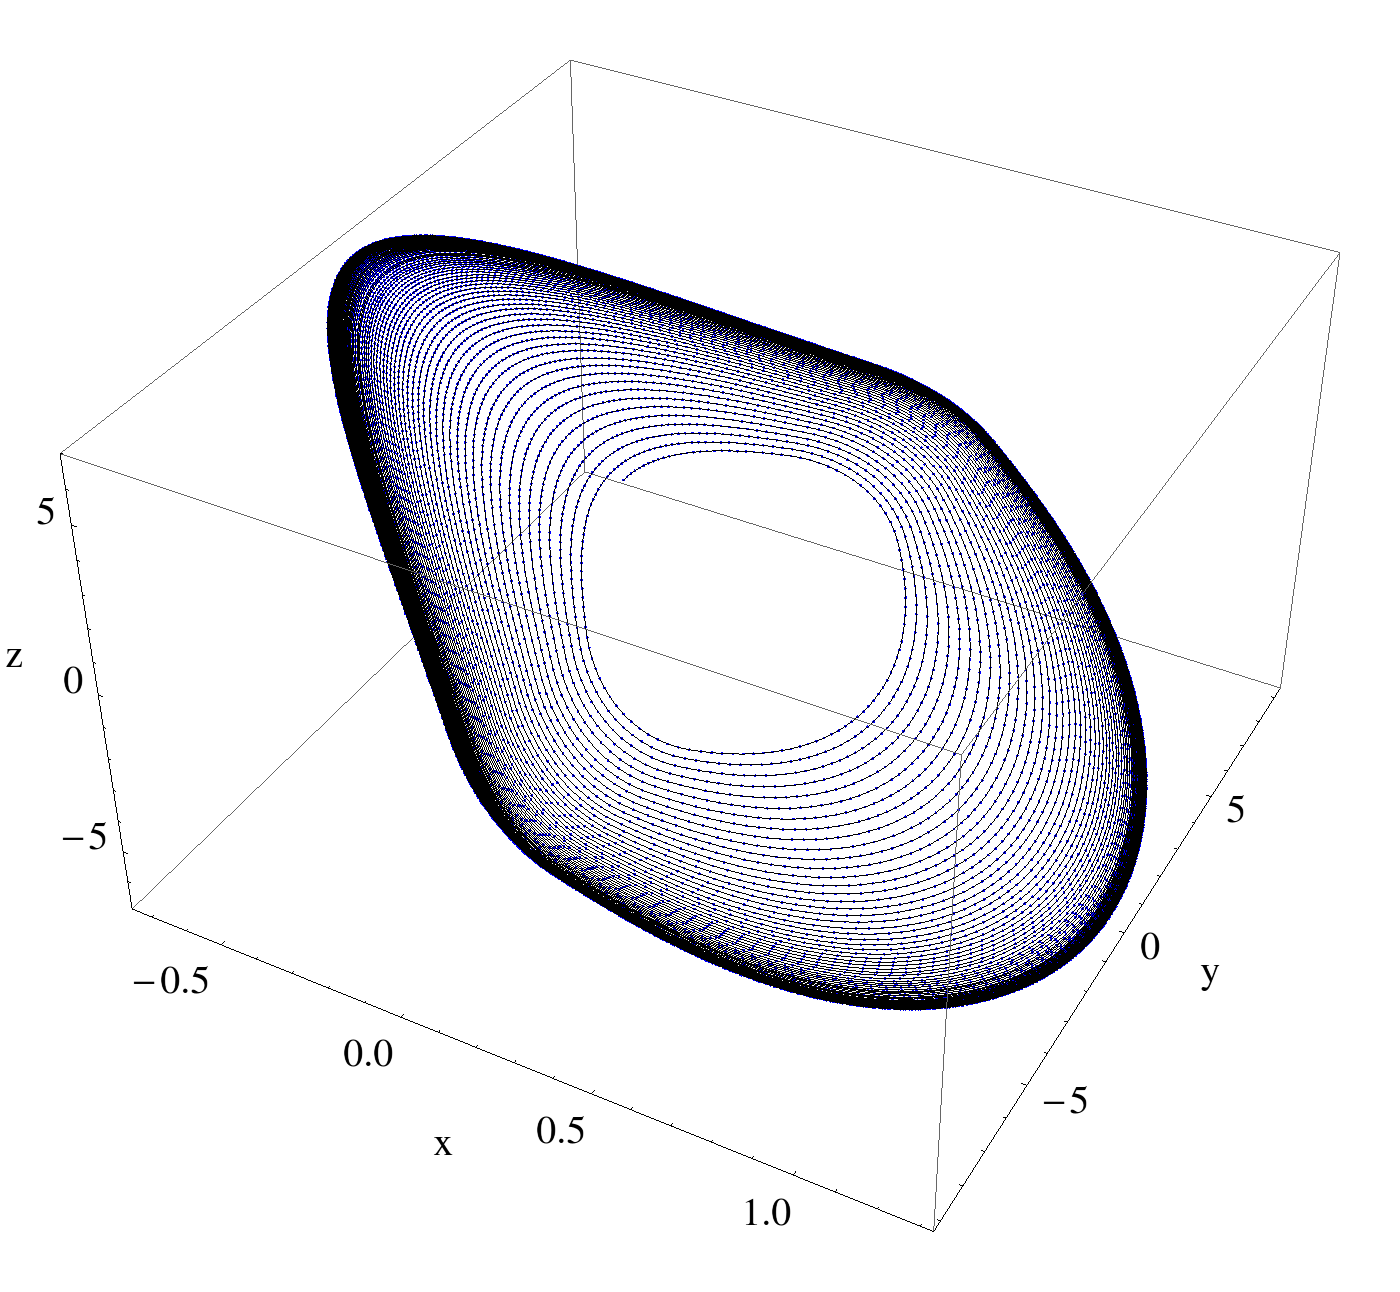
\includegraphics[width=0.45\textwidth]{model-organisms/model-leg/Modelleg-0g-100s-friction11-force0-7-damping0-05-xyz.png}
};

\node[align=left] at (9,0){\underline{Joint Dynamics}};
\node[inner sep=0pt] (joint-dynamics) at (9,-3)
{
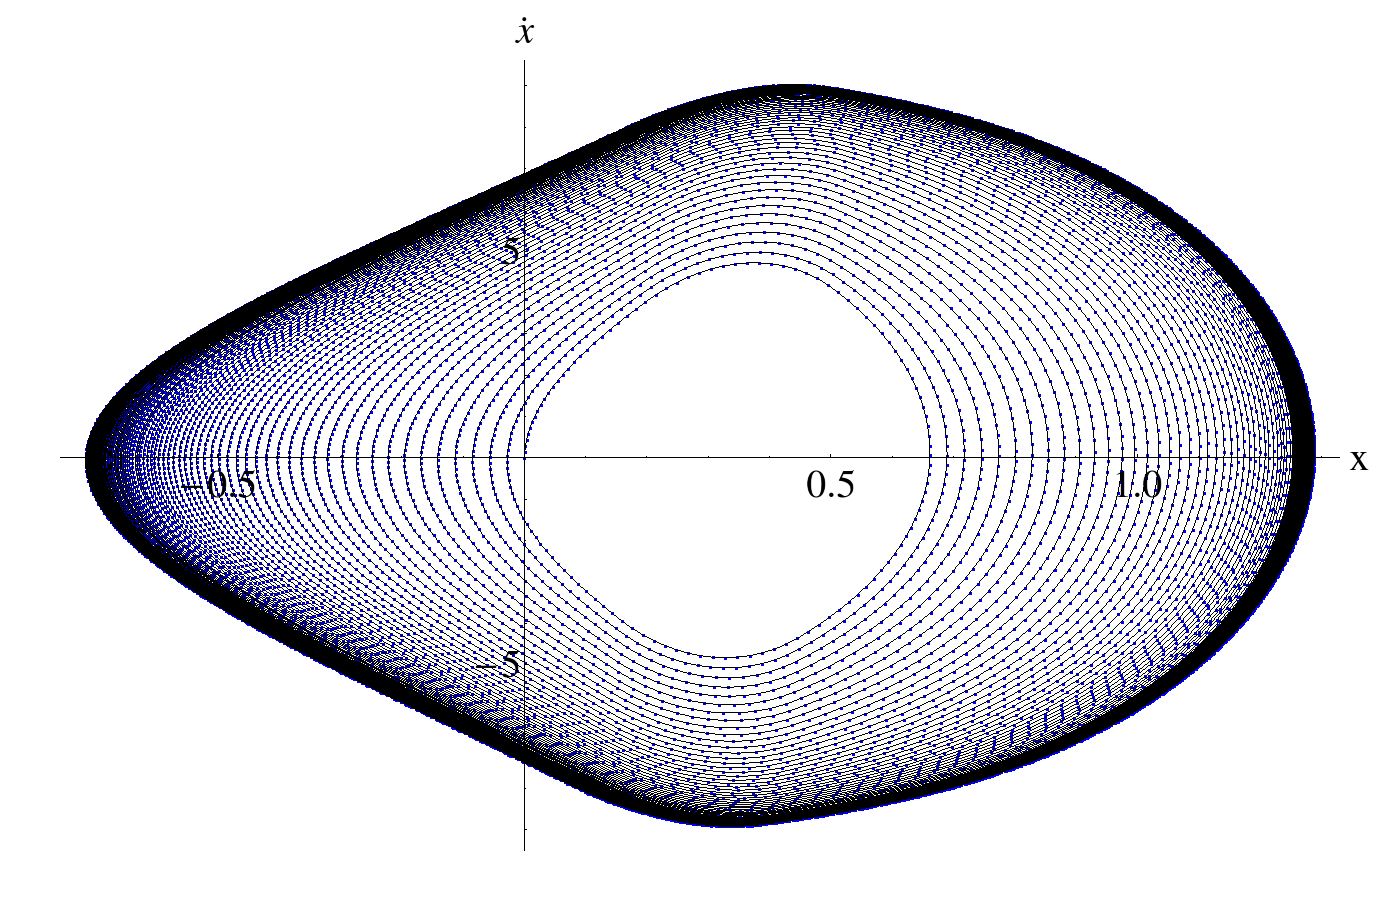
\includegraphics[width=0.45\textwidth]{model-organisms/model-leg/Modelleg-0g-100s-friction11-force0-7-damping0-05-xyz-joint.png}
};
	\end{tikzpicture}
	\end{minipage}
	\caption[Damped, limited chaotic controller controlling model leg]{The damping of the model leg softens the curvature of the periodic orbit.}
	\begin{tabular}{l|ll}
	\hline 
	Gravity: 0g  & Sensors: & Joint position \(\rightarrow\) x(t),\\
	 Output: z(t) \(\rightarrow\) Joint torque & & Joint Velocity \(\rightarrow\) y(t) \\
	  Torque scaling curve: \(0.7~(mass_1~\cdot~mass_2)\) & Damping: & 0.05 \\
	  \hline
	\end{tabular}

	\label{figure:limited-damped-model-leg-damping1}
\end{figure}

Gradually increasing the joint torque shows that the convergence to the limit cycle is increased and the original curvature of the periodic orbit comes back.

\begin{figure}[H]
	\centering
	\begin{minipage}{1.3\textwidth}
	\hspace*{-5em}
	\begin{tikzpicture}

% classes
\pgfdeclarelayer{background}
\pgfdeclarelayer{foreground}
\pgfsetlayers{background,main,foreground}
\tikzstyle{bigbox} = [draw=black!80, thick, fill=black!5, rounded corners, rectangle]
\tikzstyle{box} = [minimum size=0.6cm, rounded corners,rectangle, fill=black!50]

\node[align=left] at (0,0){\underline{Controller State Space}};
\node[inner sep=0pt] (controller-state-space) at (0,-3)
{
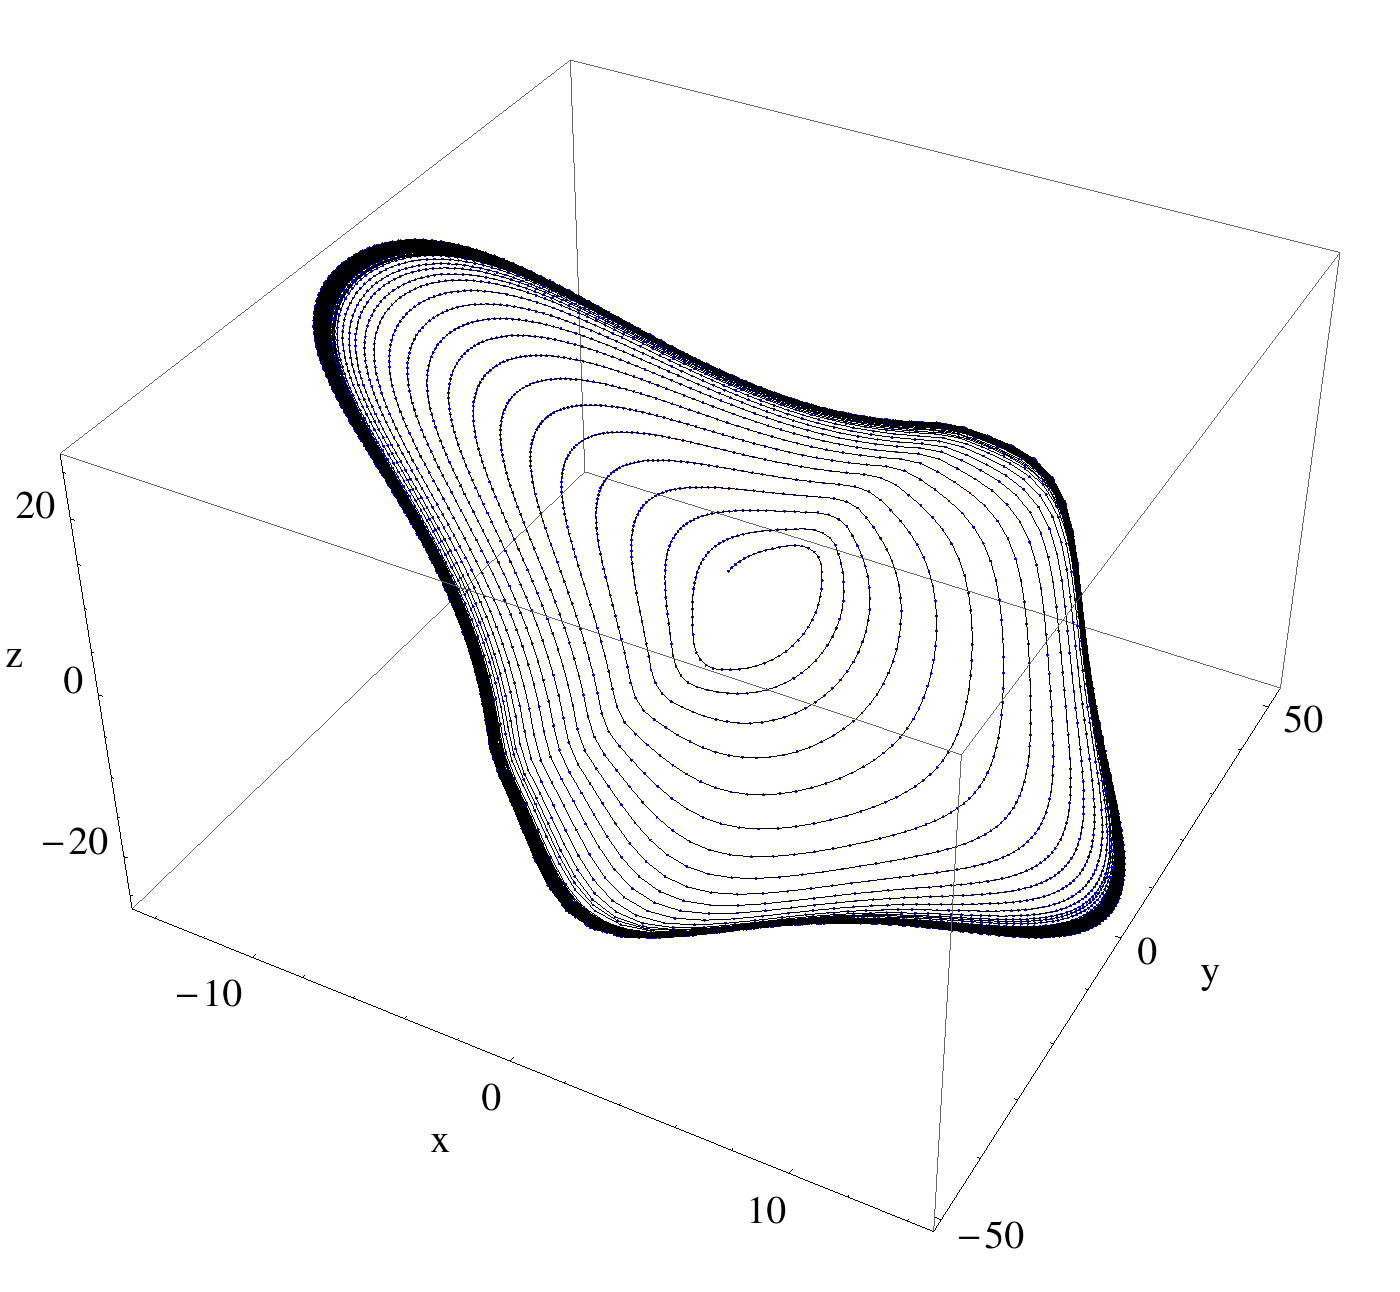
\includegraphics[width=0.45\textwidth]{model-organisms/model-leg/Modelleg-0g-100s-friction11-force4-damping0-05-(x)yz.png}
};

\node[align=left] at (9,0){\underline{Joint Dynamics}};
\node[inner sep=0pt] (joint-dynamics) at (9,-3)
{
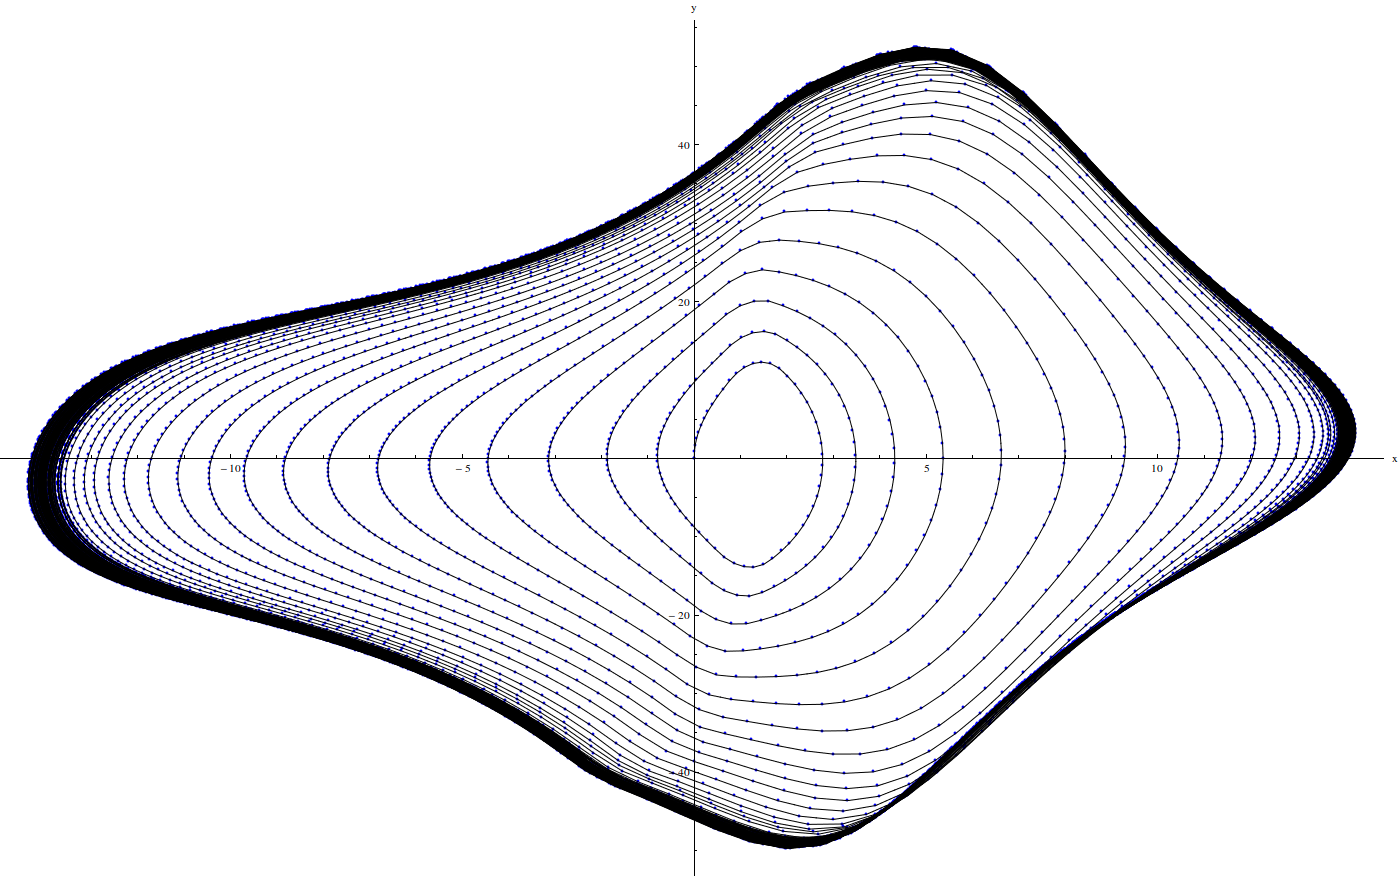
\includegraphics[width=0.45\textwidth]{model-organisms/model-leg/Modelleg-0g-100s-friction11-force4-damping0-05-(x)yz-joint.png}
};
	\end{tikzpicture}
	\end{minipage}
	\caption[Damped, torque increased, limited chaotic controller controlling model leg]{The convergence speed of the trajectory to the periodic orbit is increased, additionally the system again convergence to a curvature similar to the one without damping.}
	\begin{tabular}{l|ll}
	\hline 
	Gravity: 0g  & Sensors: & Joint position \(\rightarrow\) x(t),\\
	 Output: z(t) \(\rightarrow\) Joint torque &  & Joint Velocity \(\rightarrow\) y(t) \\
	  Torque scaling curve: \(4~(mass_1~\cdot~mass_2)\) & Damping: & 0.05 \\
	  \hline
	\end{tabular}

	\label{figure:limited-damped-model-leg-damping2}
\end{figure}

\begin{figure}[H]
	\centering
	\begin{minipage}{1.3\textwidth}
	\hspace*{-5em}
	\begin{tikzpicture}

% classes
\pgfdeclarelayer{background}
\pgfdeclarelayer{foreground}
\pgfsetlayers{background,main,foreground}
\tikzstyle{bigbox} = [draw=black!80, thick, fill=black!5, rounded corners, rectangle]
\tikzstyle{box} = [minimum size=0.6cm, rounded corners,rectangle, fill=black!50]

\node[align=left] at (0,0){\underline{Controller State Space}};
\node[inner sep=0pt] (controller-state-space) at (0,-3)
{
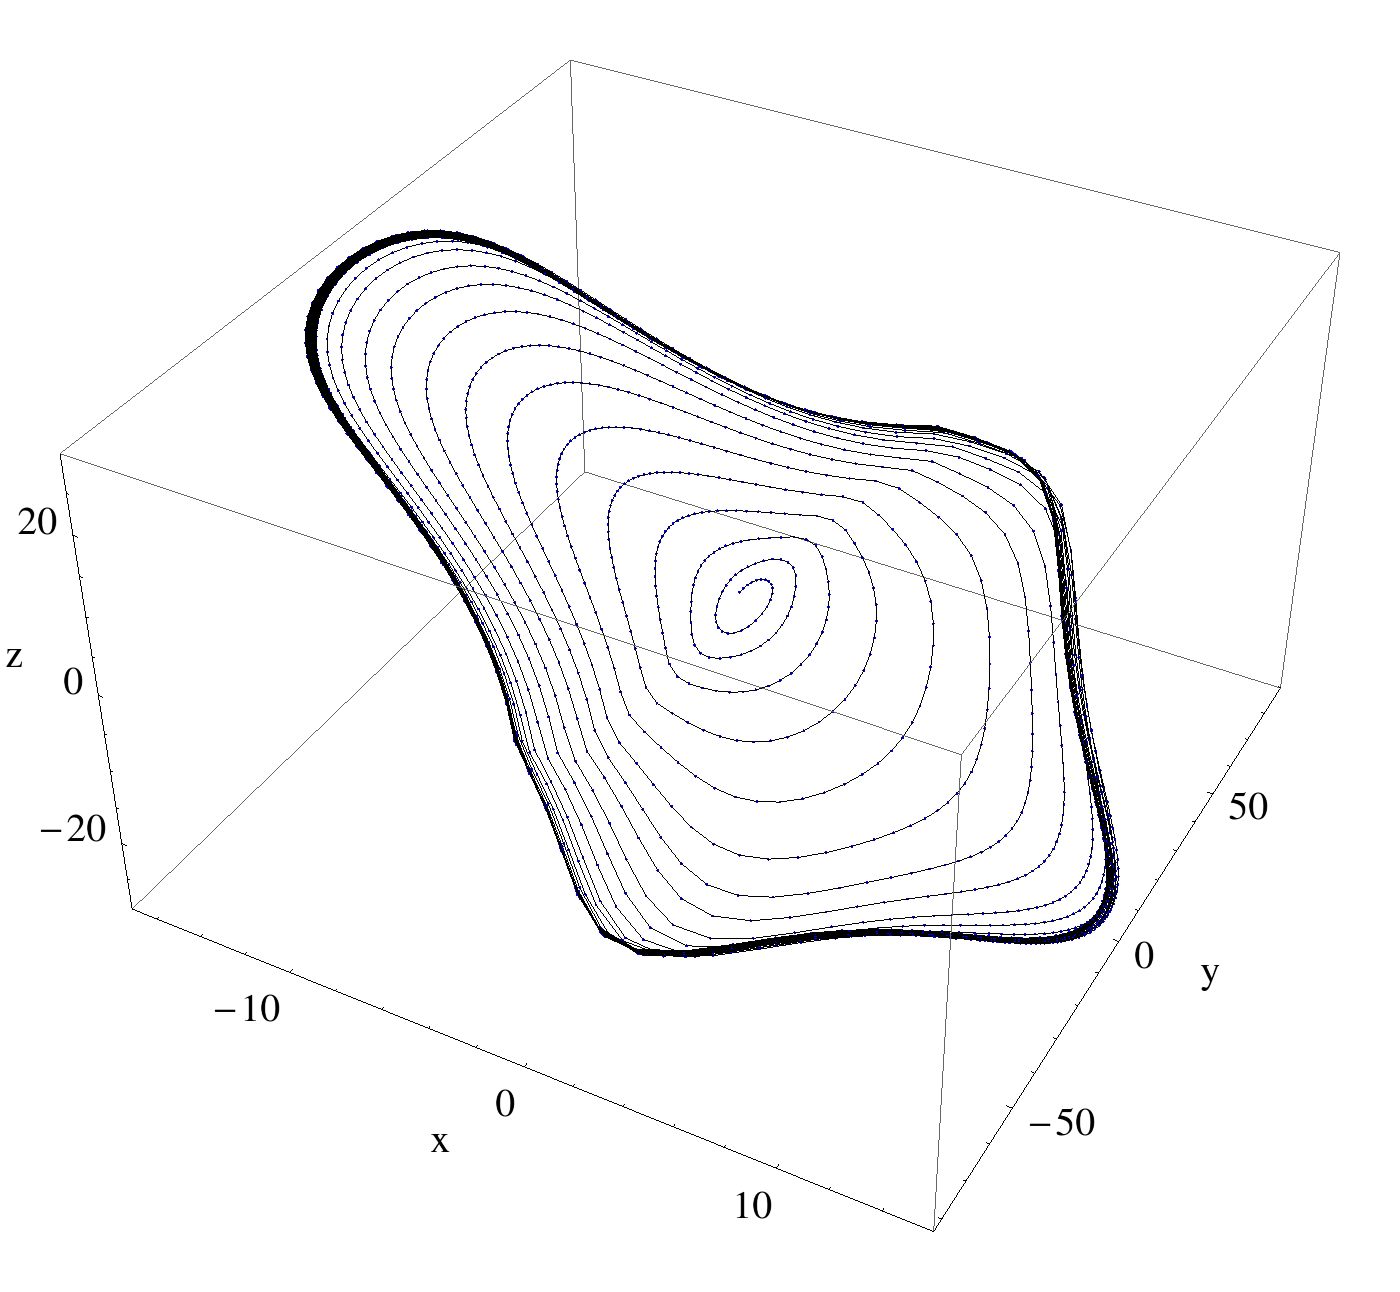
\includegraphics[width=0.45\textwidth]{model-organisms/model-leg/Modelleg-0g-100s-friction00-force10-damping0-05-(x)yz(0-7).png}
};

\node[align=left] at (9,0){\underline{Joint Dynamics}};
\node[inner sep=0pt] (joint-dynamics) at (9,-3)
{
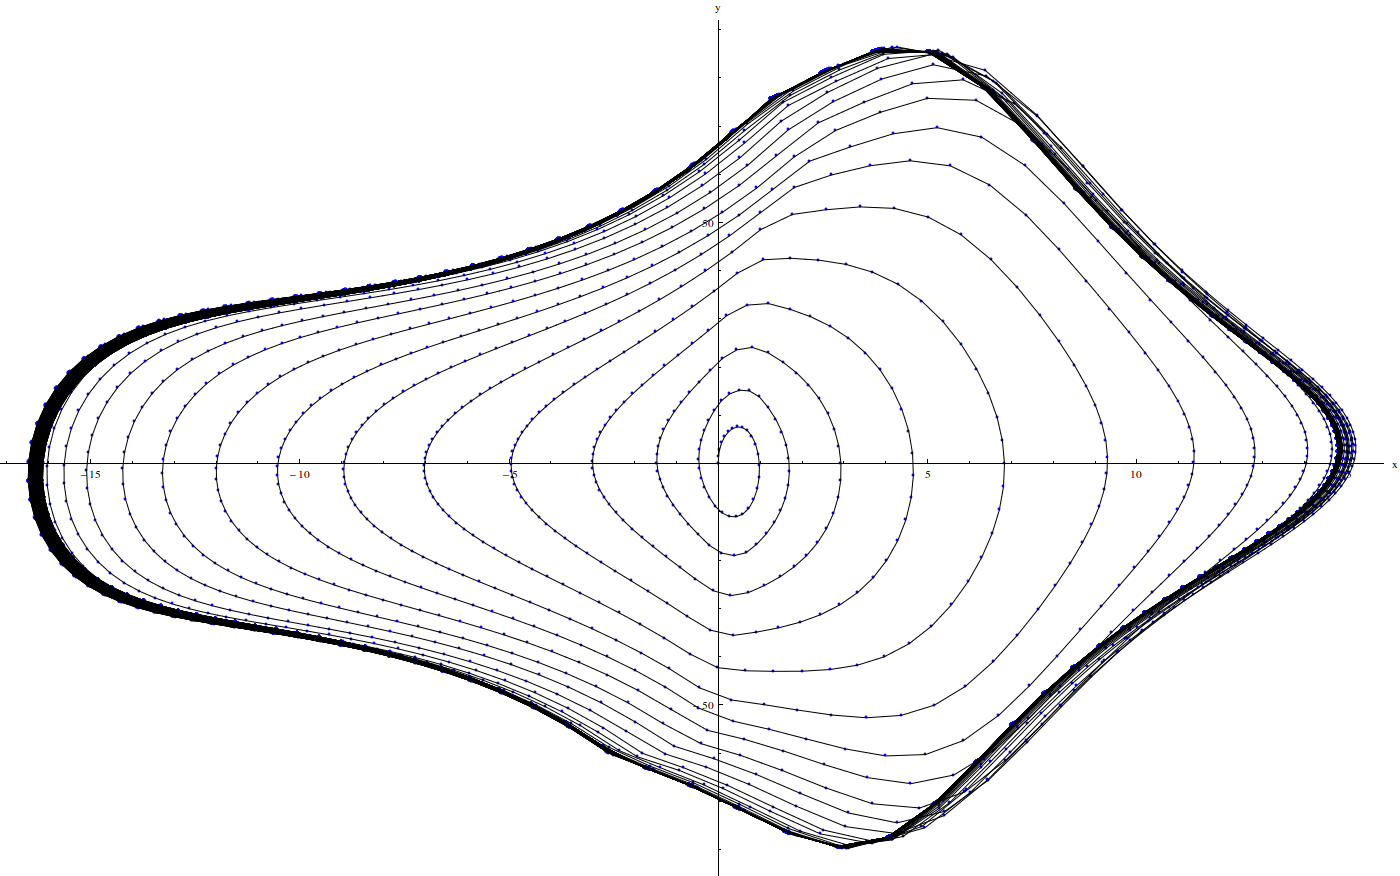
\includegraphics[width=0.45\textwidth]{model-organisms/model-leg/Modelleg-0g-100s-friction00-force10-damping0-05-(x)yz(0-7)-joint.png}
};
	\end{tikzpicture}
	\end{minipage}
	\caption[Damped, torque increased, limited chaotic controller controlling model leg]{Increasing the torque again increases the convergence speed again.}
	\begin{tabular}{l|ll}
	\hline 
	Gravity: 0g  & Sensors: & Joint position \(\rightarrow\) x(t),\\
	 Output: z(t) \(\rightarrow\) Joint torque &  & Joint Velocity \(\rightarrow\) y(t) \\
	  Torque scaling curve: \(10~(mass_1~\cdot~mass_2)\) & Damping: & 0.05 \\
	  \hline
	\end{tabular}

	\label{figure:limited-damped-model-leg6-damping3}
\end{figure}

If more torque and more damping is applied, a higher convergence speed can be observed. The trajectory again stays in a much smaller sub-manifold.

\begin{figure}[H]
	\centering
	\begin{minipage}{1.3\textwidth}
	\hspace*{-5em}
	\begin{tikzpicture}

% classes
\pgfdeclarelayer{background}
\pgfdeclarelayer{foreground}
\pgfsetlayers{background,main,foreground}
\tikzstyle{bigbox} = [draw=black!80, thick, fill=black!5, rounded corners, rectangle]
\tikzstyle{box} = [minimum size=0.6cm, rounded corners,rectangle, fill=black!50]

\node[align=left] at (0,0){\underline{Controller State Space}};
\node[inner sep=0pt] (controller-state-space) at (0,-3)
{
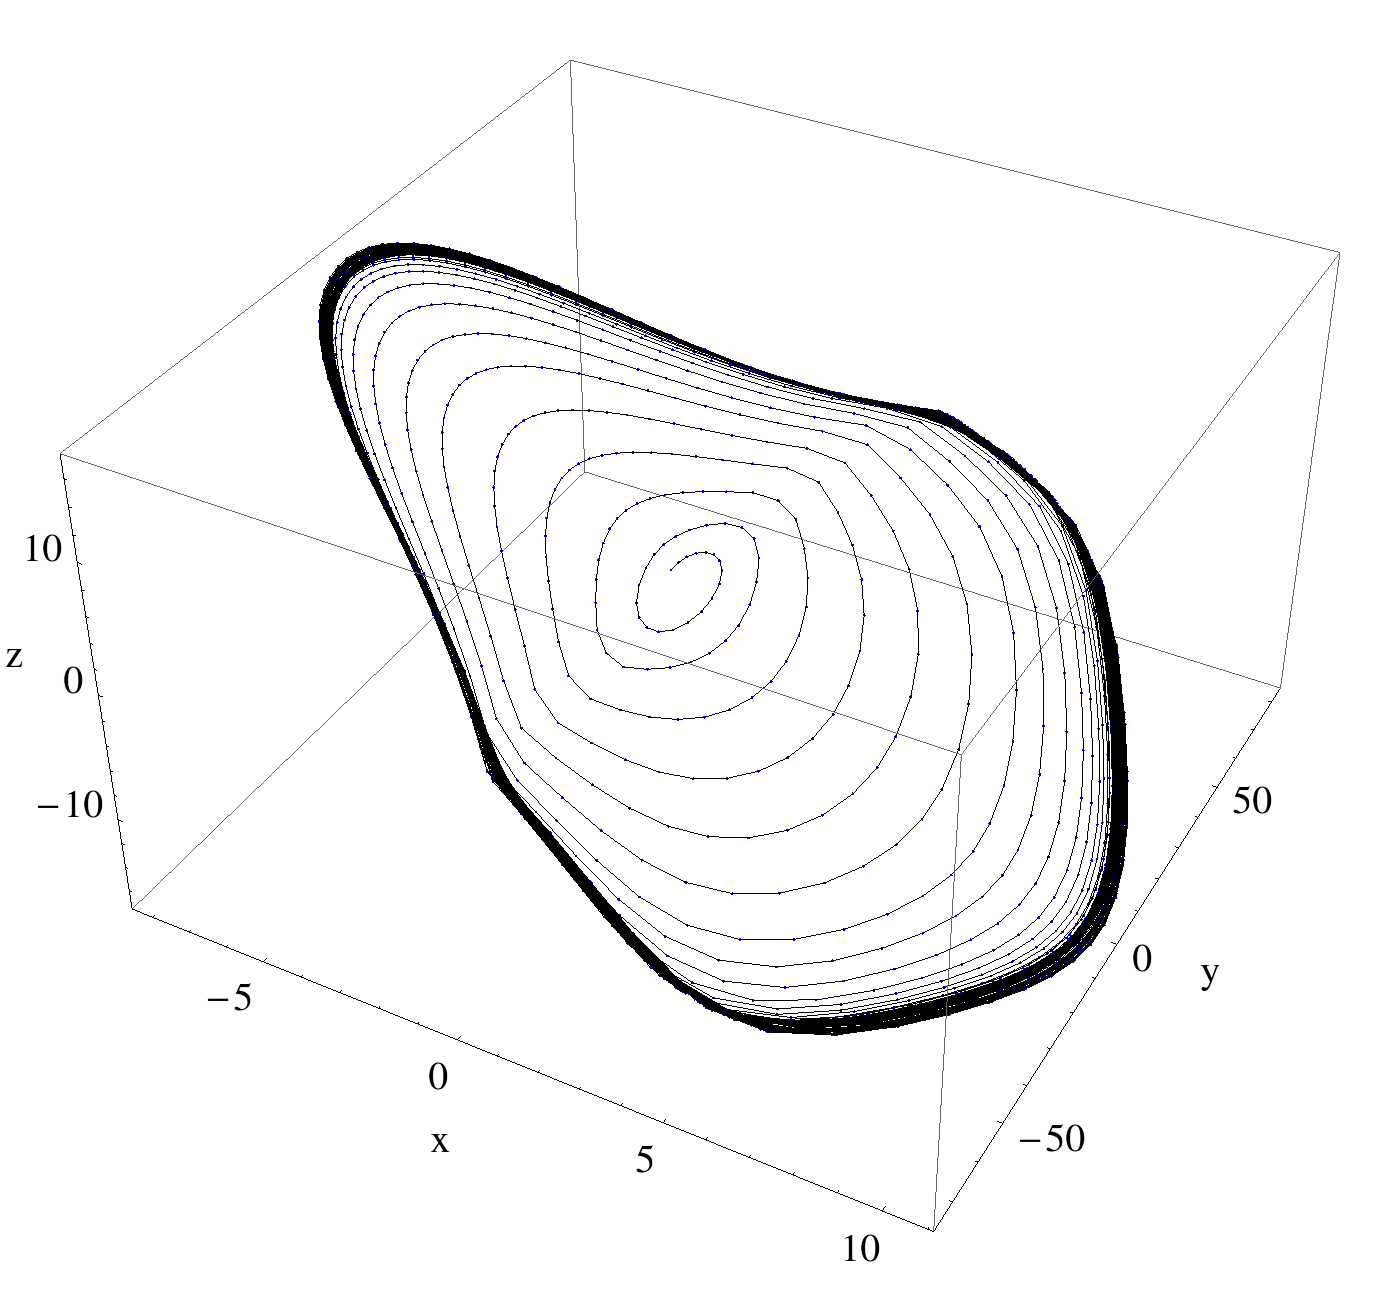
\includegraphics[width=0.45\textwidth]{model-organisms/model-leg/Modelleg-0g-100s-friction00-force20-damping5-(x)yz(0-7).png}
};

\node[align=left] at (9,0){\underline{Joint Dynamics}};
\node[inner sep=0pt] (joint-dynamics) at (9,-3)
{
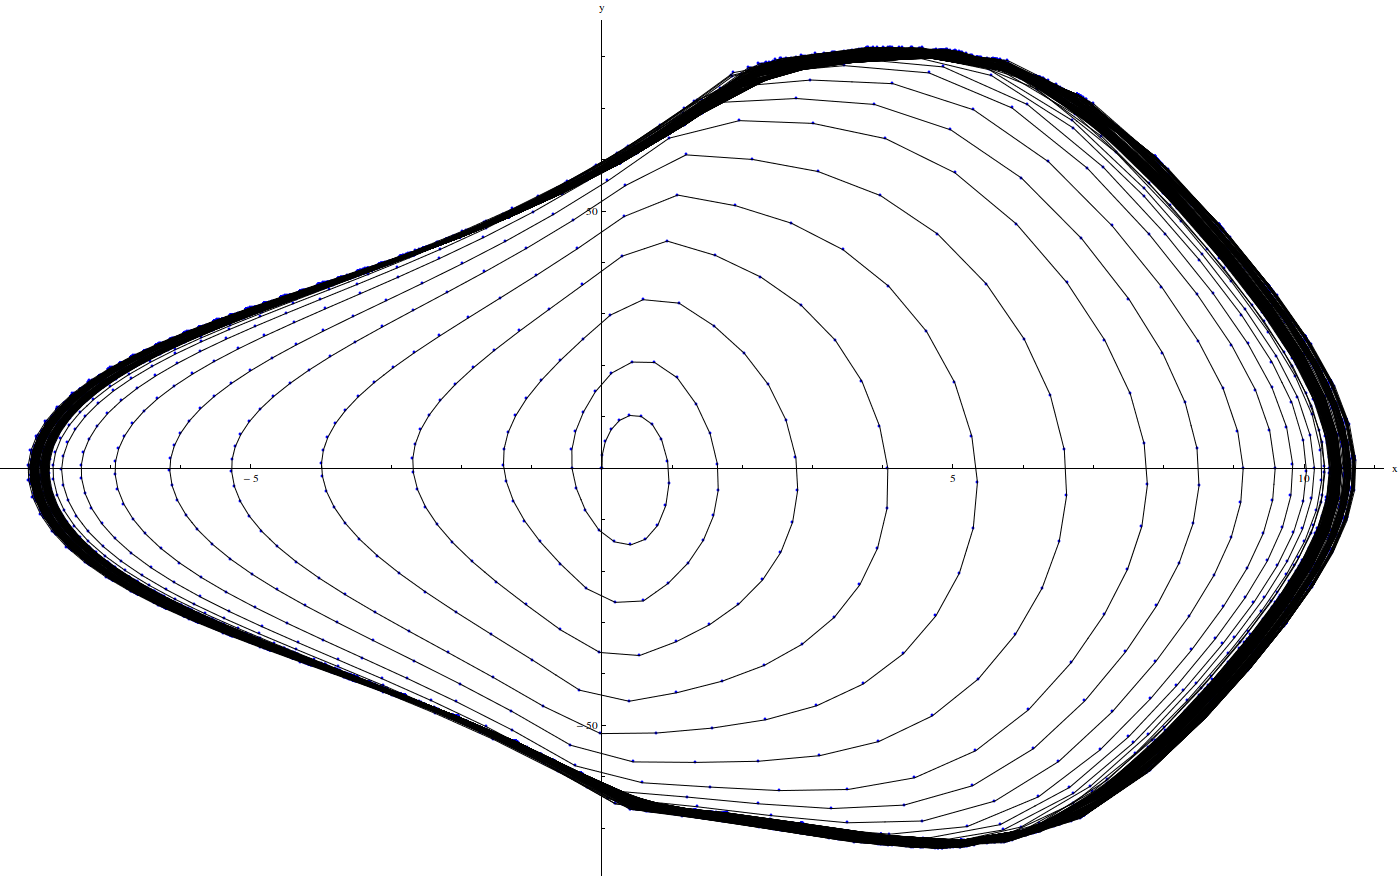
\includegraphics[width=0.45\textwidth]{model-organisms/model-leg/Modelleg-0g-100s-friction00-force20-damping5-(x)yz(0-7)-joint.png}
};
	\end{tikzpicture}
	\end{minipage}
	\caption[Highly damped, torque strongly increased, limited chaotic controller controlling model leg]{With more torque and more damping, the trajectory converges quickly to the periodic orbit.}
	\begin{tabular}{l|ll}
	\hline 
	Gravity: 0g  & Sensors: & Joint position \(\rightarrow\) x(t),\\
	 Output: z(t) \(\rightarrow\) Joint torque &  & Joint Velocity \(\rightarrow\) y(t) \\
	  Torque scaling curve: \(20~(mass_1~\cdot~mass_2)\) & Damping: & 5 \\
	  \hline
	\end{tabular}

	\label{figure:limited-damped-model-leg-damping4}
\end{figure}

Conclusively, the damping of the system leads to a smoother limit cycle of the original system's trajectory, however, still converges to a limit cycle, even if more force and more damping is applied.

\paragraph{Influence of the X Dimension Limiter} From the initial experiments on limiter configuration (\ref{figure:limited-model-leg5}), it is known that the velocity sensor limiting the y dimension could have been sufficient for the limiter control of the chaotic system. %
%
One can now observe the influence of the x dimension limiter when it is removed from the system. In this case, the initial conditions were set to \([0,0,0]\) to observe the complete trajectory.

\begin{figure}[H]
	\centering
	\begin{minipage}{1.3\textwidth}
	\hspace*{-5em}
	\begin{tikzpicture}

% classes
\pgfdeclarelayer{background}
\pgfdeclarelayer{foreground}
\pgfsetlayers{background,main,foreground}
\tikzstyle{bigbox} = [draw=black!80, thick, fill=black!5, rounded corners, rectangle]
\tikzstyle{box} = [minimum size=0.6cm, rounded corners,rectangle, fill=black!50]

\node[align=left] at (0,0){\underline{Controller State Space}};
\node[inner sep=0pt] (controller-state-space) at (0,-3)
{
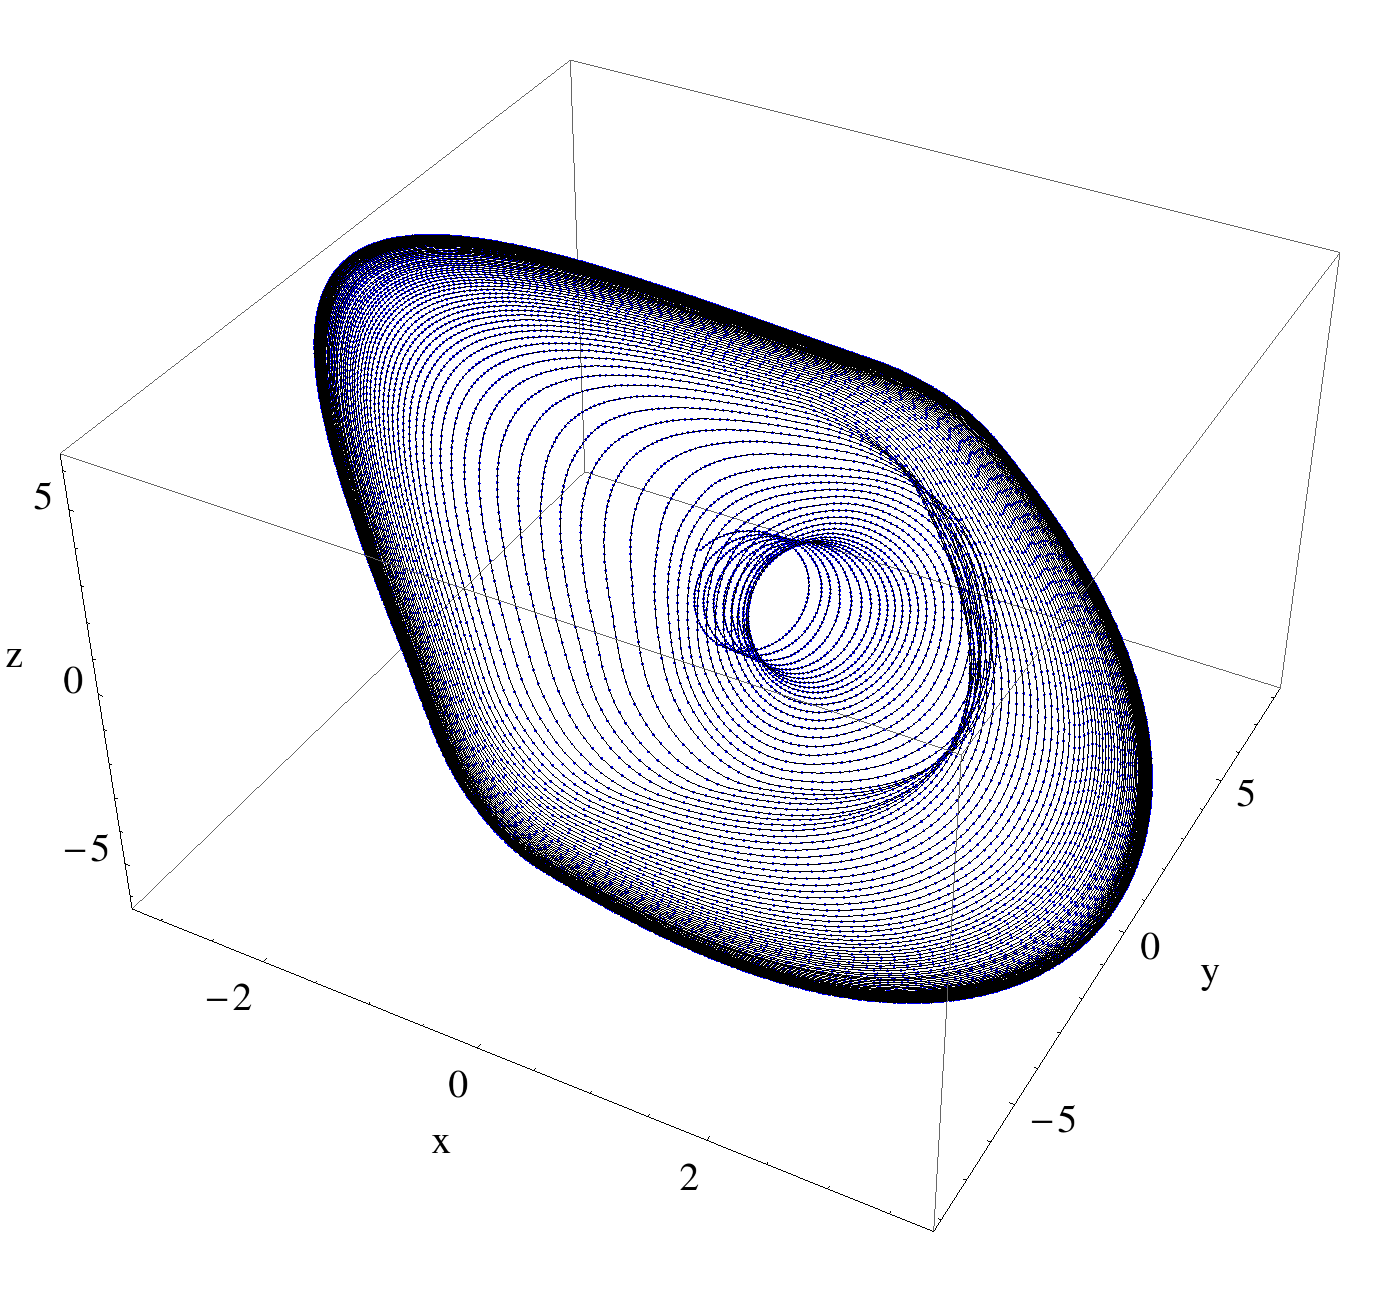
\includegraphics[width=0.45\textwidth]{model-organisms/model-leg/Modelleg-0g-100s-friction00-force0-7-damping0-05-(x)yz(0-7).png}
};

\node[align=left] at (9,0){\underline{Joint Dynamics}};
\node[inner sep=0pt] (joint-dynamics) at (9,-3)
{
\includegraphics[width=0.45\textwidth]{model-organisms/model-leg/Modelleg-0g-100s-friction00-force0-7-damping0-05-(x)yz(0-7)-joint.png}
};
	\end{tikzpicture}
	\end{minipage}
	\caption[Limited chaotic controller controlling model leg]{}
	\begin{tabular}{l|ll}
	\hline 
	Gravity: 0g  & Sensors: & Joint Velocity \(\rightarrow\) y(t)\\
	 Output: z(t) \(\rightarrow\) Joint torque & & - \\
	  Torque scaling curve: \(0.7~(mass_1~\cdot~mass_2)\) & Damping: & 0.05 \\
	  \hline
	\end{tabular}

	\label{figure:limited-damped-model-leg8}
\end{figure}

If the system gets one of its degrees of freedom back, it shows some of its internal dynamics. However, the original convergence behavior still occurs.

In conclusion it can be said that the stronger a chaotic system is limited through the output from another dynamical system, the more it exhibits similar patterns as the dynamical system it is limited by. Since in these experiments the Chua circuit is under a constant limiter from the joint dynamics, it can only emit a limited range of mostly periodic trajectories.

\subsubsection{Evolved Creatures with Direct Limiter Control}
\label{subsec:Evolved-lim-creatures}

The setup to evolve creatures integrating the chaotic controllers was intended to be an exploratory one. %
%
In order to observe examples of creatures that locomote using chaotic controllers, three simulators with each a separate evolutionary setting were started. %
%
Each setting has 100 individuals in one population, each with the same average velocity fitness function. %
%
This setup was chosen through the single fitness function in a very liberal way, so that different creatures could evolve their own dynamics, because so many locomotion solutions are possible to be evolved. %
%
The simulators were run on a quad-core processor system, so the multiple simulators exploited the multiple cores much better than a single simulator could. %
%
The experiment using the direct limiter controller chaotic controller sounded much more promising, since the controller stayed in a quasi-periodic motion for all the time for almost all the model leg setups. %
%
Its output seemingly could be easily compared to the sinusoidal controllers. %
%
This assumption turns out to be quite false in practice, because when integrated into random morphologies by the evolutionary algorithm, the controller exhibits periodic motion at some point when limited appropriately. %
%
But in other cases, the controllers switches to a different periodic or non-periodic trajectory when influenced by the environment. %
% 
Thus, a controller might sometimes stabilize a periodic orbit at one point, but remain in a chaotic state at all others. %

\begin{figure}[H]
\centering
\includegraphics[width=0.9\textwidth]{results/evolved-creatures/chaotic/chaotic-periodic-switching.png}
\caption[Chaotic-periodic phase switching]{A plot of the controller phase space showing a trajectory containing interweaving chaotic and periodic phases.}
\label{figure:z-2.4-3.19-chaotictrajectories}
\end{figure}

The simple limiters of the environment apparently stabilize a certain periodic orbit, but change, when the environment changes. %
%
The controller therefore satisfies the idea of being adaptive to the environment, however it stayed in question if multiple controllers could be combined with a co-evolved morphology so that a satisfactory locomotion pattern would arise. %
%
The fitness function of average velocity totally leaves it up to the individual, how the movement would be achieved. %
%
Evolutionary algorithms are very exploitive, meaning that the evolved solutions easily exploit everything they can find to satisfy the fitness functions. %
%
However, the strength of the evolutionary algorithm, its versatility to find solutions, turns in this case into a very messy task for the experimenter. %
%
For higher order tasks such as locomotion, it means that one has to come up with a simple but precise description of the solution space using fitness functions. %
%
The definition must be general enough to accept a variety of solutions, but must be precise enough to accept only the desired solutions. %
%
What sounds easy for simple tasks, is not very easy for more complex tasks. %
%
One might argue here that the question here is really what locomotion actually is. %
%
When defined as being an action causing directed movement, then nearly everything is allowed to be evolved. %
%
On the other end, restricting locomotion to body parts being moved in coordination to form complex oscillatory gaits, then only very few solutions fit the description. %
%
In this thesis, the definition was kept very loose, so that most solutions involving oscillatory actions causing directed movement can be considered locomotion. %
%
Therefore, the first simulations were started with the average velocity fitness function only. %
%
After 500 generations of simulated evolution, the simulators were stopped and the evolved creatures were examined. %
%
The definition was not at all sufficient to evolve locomoting creatures. %
%
Some of them were moving, but evolved into larger balls with many legs, so that the oscillatory movement caused the structure to roll. %
%
Some of them even just exploited the fact that growing tall and falling over causes them to slide a certain distance, resulting in a substantial average velocity. %
%
Because the results were not desirable, the experiment was redesigned to cope with the definition problem. %
%
The definition was changed multiple times after examining the evolved creatures. %
%
As long as the creatures showed hints to converge onto the desired behavior, the simulation was continued without changes, otherwise, the definition was changed again. %
%
The best results were achieved using a stronger restriction on the solutions, which was a combination of the average velocity fitness function and a minimal contact point quantity fitness function. %
%
The minimal contact point quantity fitness function reduced the the number of feet a creature develops, therefore a clearer locomotion pattern had to emerge. %
%
In the following figures, three of these evolved creatures are examined in detail.

\paragraph{Walker}

The first creature is a walker. It has two large feet, of which it always moves one forward while using the other as a stabilization. 

\begin{figure}[H]
\centering
\includegraphics[width=0.95\textwidth]{results/evolved-creatures/chaotic/walker1/walker1-animation.png}
%\includegraphics[width=0.45\textwidth]{results/evolved-creatures/chaotic/walker1/014.png}
%\includegraphics[width=0.45\textwidth]{results/evolved-creatures/chaotic/walker1/029.png}
%\includegraphics[width=0.45\textwidth]{results/evolved-creatures/chaotic/walker1/036.png}
%\includegraphics[width=0.45\textwidth]{results/evolved-creatures/chaotic/walker1/069.png}
%\includegraphics[width=0.45\textwidth]{results/evolved-creatures/chaotic/walker1/116.png}
%\includegraphics[width=0.45\textwidth]{results/evolved-creatures/chaotic/walker1/120.png}
\caption[Figure of a walker using chaotic controllers.]{A figure of a walker featuring 4 chaotic controllers and 4 joints. It has two large feet it stands on, which push the body forward. In the front of the creature there is a stabilizing block that in certain cases touches the ground if the creature tips during its gait. A video of the walking creature can be found on YouTube: \url{https://youtu.be/jwaEXxB7ZB4}.}
\label{figure:successfulcreatures-chaotic-walker1}
\end{figure}

The first creature features quasi-periodic orbits if the body parts are not limited by the ground. %
%
The quasi periodicity can be explained by the interdynamics generated by the different body parts moving simultaneously, therefore no single body part can follow a proper limit cycle. %

\begin{figure}[H]
\centering
\includegraphics[width=0.8\textwidth]{results/evolved-creatures/chaotic/walker1/limitless-dynamics.png}
\caption[Off ground controller dynamics of the walker]{Dynamics of a chaotic controller if the walker is off ground.}
\label{figure:walker1-off-ground-controller-dynamics}
\end{figure}

The same controller features chaotic and quasi-periodic dynamics if limited by the ground. %

\begin{figure}[H]
\centering
\includegraphics[width=0.8\textwidth]{results/evolved-creatures/chaotic/walker1/limited-dynamics.png}
\caption[On ground controller dynamics of the walker]{Dynamics of a chaotic controller if the walker is on ground.}
\label{figure:walker1-on-ground-controller-dynamics}
\end{figure}

This behavior can be explained because the gait of the creature always traps one leg while moving the other, then the behavior switches to the other leg. %
%
This leads to a chaotic trajectory in the controller when the leg is completely trapped, and to a periodic trajectory when untrapped. %

\paragraph{Crawler}

The second creature is a crawler. It moves on ground using a gait similar to a snake by oscillating its tail.

\begin{figure}[H]
\centering
\includegraphics[width=0.85\textwidth]{results/evolved-creatures/chaotic/crawler1/crawler1-animation.png}
%\includegraphics[width=0.45\textwidth]{results/evolved-creatures/chaotic/crawler1/140.png}
%\includegraphics[width=0.45\textwidth]{results/evolved-creatures/chaotic/crawler1/143.png}
%\includegraphics[width=0.45\textwidth]{results/evolved-creatures/chaotic/crawler1/149.png}
%\includegraphics[width=0.45\textwidth]{results/evolved-creatures/chaotic/crawler1/163.png}
\caption[Figure of a crawler using chaotic controllers.]{Top-down view of a crawler featuring 10 chaotic controllers and 10 joints. The crawler has a tail and two arms looking to the left and right from the head, and moves forward using a snake-like locomotion gait. A video of the crawling creature can be found on YouTube: \url{https://youtu.be/3qpJOooM4Vc}.}
\label{figure:successfulcreatures-chaotic-crawler1}
\end{figure}

When off ground, the controllers of the creature show a chaotic oscillation behavior. %

\begin{figure}[H]
\centering
\includegraphics[width=0.8\textwidth]{results/evolved-creatures/chaotic/crawler1/limitless-dynamics-2.png}
\caption[Off ground controller dynamics of the crawler]{Dynamics of a chaotic controller if the crawler is off ground.}
\label{figure:crawler1-off-ground-controller-dynamics}
\end{figure}

The same controller features a different kind of chaotic behavior when on ground. %

\begin{figure}[H]
\centering
\includegraphics[width=0.8\textwidth]{results/evolved-creatures/chaotic/crawler1/limited-dynamics-2.png}
\caption[On ground controller dynamics of the crawler]{Dynamics of a chaotic controller if the crawler is on ground.}
\label{figure:crawler1-on-ground-controller-dynamics}
\end{figure}

\paragraph{Jumper}

The third creature is a jumper. It moves on ground by moving its body parts to gain momentum, which makes the main body finally lift off and take a small leap forward.

\begin{figure}[H]
\centering
\includegraphics[width=0.85\textwidth]{results/evolved-creatures/chaotic/jumper1/jumper1-animation.png}
%\includegraphics[width=0.45\textwidth]{results/evolved-creatures/chaotic/jumper1/457.png}
%\includegraphics[width=0.45\textwidth]{results/evolved-creatures/chaotic/jumper1/542.png}
%\includegraphics[width=0.45\textwidth]{results/evolved-creatures/chaotic/jumper1/645.png}
%\includegraphics[width=0.45\textwidth]{results/evolved-creatures/chaotic/jumper1/685.png}
\caption[Figure of a jumper using chaotic controllers.]{Figure of a jumper featuring 10 chaotic controllers and 10 joints. The jumper has several legs it uses to accumulate momentum in order to jump forward. A video of the jumping creature can be found on YouTube: \url{https://youtu.be/JyBFdD_wCoQ}.}
\label{figure:successfulcreatures-chaotic-crawler1}
\end{figure} 

When off ground, the controllers of the creature show a chaotic oscillation behavior. %

\begin{figure}[H]
\centering
\includegraphics[width=0.8\textwidth]{results/evolved-creatures/chaotic/jumper1/c4-off-ground.png}
\caption[Off ground controller dynamics of the crawler]{Dynamics of a chaotic controller if the jumper is off ground.}
\label{figure:crawler1-off-ground-controller-dynamics}
\end{figure}

The same controller features a limit cycle which seems to be limited in the lower right corner of the plot when on ground. %

\begin{figure}[H]
\centering
\includegraphics[width=0.8\textwidth]{results/evolved-creatures/chaotic/jumper1/c4-on-ground.png}
\caption[On ground controller dynamics of the crawler]{Dynamics of a chaotic controller if the jumper is on ground.}
\label{figure:crawler1-on-ground-controller-dynamics}
\end{figure}

All three creatures show adaptive behavior depending on whether they are on ground or off ground. %
%
However, the influence of the limiters are not always of the prominent nature of the simple limiter. %
%
A simple measure of gait stability is the distance travelled by the creature. %
%
If the distance drops strongly when the gait is perturbed, the creature must have been strongly influenced by the perturbance (i.e. it has fallen over or has diverged strongly from its initial walk). %
%
To get a qualitative measure of stability, all controllers of the three creatures were perturbed in the beginning of their evaluation using small uniformly distributed zero mean perturbances of amplitude \([0,1 \cdot 10^{-8}]\) to see if the travelled distance varies. %
%
The perturbation experiment was repeated 100 times for each creature, however the locomoted distance varied less than \(\unit[1]{\%}\) for all of the runs. %
\end{document}